\begin{filecontents*}{referencias.bib}
@book{Netto2003,
	author    = {Paulo Oswaldo Boaventura Netto},
	title     = {Grafos: teoria, modelos, algoritmos},
	year      = {2003},
	publisher = {Editora Blucher},
	location  = {São Paulo}
}

@mastersthesis{Pereira2021,
	author   = {Wanderson Douglas Lomenha Pereira},
	title    = {Decomposição de grafos em subgrafos localmente irregulares},
	type     = {Dissertação (Mestrado em Engenharia de Sistemas e Computação)},
	school   = {COPPE/UFRJ},
	address  = {Rio de Janeiro},
	year     = {2021},
	month    = apr,
	url      = {https://www.pesc.coppe.ufrj.br/uploadfile/publicacao/2990.pdf},
	urldate  = {2025-08-28}
}

@online{OliveiraRangelAraujo_OperacoesGrafos_2013,
	author        = {Valeriano A. de Oliveira and Socorro Rangel and Silvio A. de Araujo},
	title         = {Teoria dos Grafos: Capítulo 6 — Operações com Grafos},
	date          = {2013},
	organization  = {IBILCE/UNESP, Departamento de Matemática Aplicada},
	url           = {https://www.ibilce.unesp.br/Home/Departamentos/MatematicaAplicada/docentes/socorro/operacoescomgrafos.pdf},
	urldate       = {2025-08-28},
	note          = {Notas de aula}
}

@online{OliveiraRangelAraujo_ConjuntosCorte_2017,
	author        = {Valeriano A. de Oliveira and Socorro Rangel and Silvio A. de Araujo},
	title         = {Teoria dos Grafos: Capítulo 14 — Conjuntos de Corte e Conectividade},
	date          = {2017},
	organization  = {IBILCE/UNESP, Departamento de Matemática Aplicada},
	url           = {https://www.ibilce.unesp.br/Home/Departamentos/MatematicaAplicada/docentes/socorro/conjuntoscorte2017.pdf},
	urldate       = {2025-08-28},
	note          = {Notas de aula}
}

@online{CESAD_UFS_Aula7_2012,
	title         = {Matemática Discreta — Aula 7: Grafos},
	organization  = {CESAD/Universidade Federal de Sergipe},
	date          = {2012},
	url           = {https://cesad.ufs.br/ORBI/public/uploadCatalago/17364316022012Matem\%C3\%A1tica_Discreta_Aula_7.pdf},
	urldate       = {2025-08-28},
	note          = {Material didático}
}

@inproceedings{RodriguesSilvaFilho2016,
	author    = {P. M. S. Rodrigues and P. A. Silva Filho},
	title     = {Quantificação das emissões de dióxido de carbono (CO2) por veículos automotores na cidade de Boa Vista/RR – 2005 a 2015},
	booktitle = {Anais do 7º Congresso Luso-Brasileiro para o Planejamento Urbano, Regional, Integrado e Sustentável (PLURIS 2016)},
	address   = {Maceió, AL},
	year      = {2016},
	url       = {https://fau.ufal.br/evento/pluris2016/files/Tema\%203\%20-\%20Mobilidade\%20e\%20Transportes/Paper1612.pdf},
	urldate   = {2025-08-28}
}

@online{Wikipedia_GraphTheory,
	author   = {{Wikipedia contributors}},
	title    = {Graph theory},
	year     = {2025},
	url      = {https://en.wikipedia.org/wiki/Graph_theory},
	urldate  = {2025-08-28},
	note     = {Wikipedia, The Free Encyclopedia}
}

@online{SigaVerde_CalculadoraFrota,
	title        = {Calcule aqui a emissão de carbono da sua frota},
	organization = {SigaVerde},
	url          = {https://www.sigaverde.com/calcule-aqui-a-emissao-de-carbono-da-sua-frota/},
	urldate      = {2025-08-28}
}

@online{LASTROP_CalculadoraEmissoes,
	title        = {Calculadora de Emissões no Transporte},
	organization = {LASTROP — ESALQ/USP},
	url          = {https://esalqlastrop.com.br/capa.asp?pi=calculadora_emissoes},
	urldate      = {2025-08-28}
}

\end{filecontents*}

\documentclass[
12pt,
a4paper,
semrecuonosumario,
sumario = abnt-6027-2012]{report}

% --- Pacotes essenciais
\usepackage[T1]{fontenc}
\usepackage[utf8]{inputenc}
\usepackage[brazil]{babel}
\usepackage{geometry}
\geometry{a4paper,margin=2.5cm}
\usepackage{setspace}
\onehalfspacing
\usepackage{graphicx}
\usepackage{float}
\usepackage[hidelinks]{hyperref}
\usepackage{titlesec}
\usepackage{tocloft}
\usepackage{helvet}
\renewcommand{\familydefault}{\sfdefault}
\usepackage{ragged2e}
\usepackage{indentfirst}
\usepackage{subcaption}
\usepackage{amsmath}
\setcounter{MaxMatrixCols}{22}
\usepackage[style=authoryear,backend=biber]{biblatex}
\usepackage{textcomp}

\addbibresource{referencias.bib}

% --- Listagens de código
\usepackage{listings}
\lstset{
	basicstyle=\ttfamily\small,
	breaklines=true,
	frame=single,
	numbers=left,
	numberstyle=\tiny,
	tabsize=2,
	literate={á}{{\'a}}1 {â}{{\^a}}1 {ã}{{\~a}}1 {à}{{\`a}}1
	{Á}{{\'A}}1 {Â}{{\^A}}1 {Ã}{{\~A}}1 {À}{{\`A}}1
	{é}{{\'e}}1 {ê}{{\^e}}1 {É}{{\'E}}1 {Ê}{{\^E}}1
	{í}{{\'i}}1 {Í}{{\'I}}1
	{ó}{{\'o}}1 {ô}{{\^o}}1 {õ}{{\~o}}1 {Ó}{{\'O}}1 {Ô}{{\^O}}1 {Õ}{{\~O}}1
	{ú}{{\'u}}1 {Ú}{{\'U}}1
	{ç}{{\c{c}}}1 {Ç}{{\c{C}}}1
}

% --- (Opcional) Lista de algoritmos – mantida para refletir o PDF
\usepackage{algorithm}
\usepackage{algpseudocode}

% --- Aparência dos títulos
% \titleformat{\chapter}{\bfseries}{\thechapter}{1em}{}
% \titleformat{\section}{\bfseries}{\thesection}{1em}{}
% \titleformat{\subsection}{\bfseries}{\thesubsection}{1em}{}

% --- Dados para a capa/rosto
\newcommand{\universidade}{UNIVERSIDADE TECNOLÓGICA FEDERAL DO PARANÁ}
\newcommand{\autores}{CAIO MACEDO\\ KAÍQUE MEDEIROS LIMA\\ IAN BATISTA FORNAZIERO}
\newcommand{\titulo}{MEMORIAL DESCRITIVO\\Algoritmos em Grafos}
\newcommand{\english}{Descriptive Memorial - Graph Algorithms}
\newcommand{\docente}{Dra. Leiliane Pereira de Rezende}
\newcommand{\cidade}{SANTA HELENA}
\newcommand{\periodo}{2025/2}

\begin{document}

% --- Capa
\begin{titlepage}
	\centering
	{\bf \universidade\par}
	\vspace{4cm}
	{\bf\autores\par}
	\vspace{6cm}
	{\bf\titulo\par}
	\vspace{9cm}
	{\bf\cidade\par}
	{\bf\periodo\par}
	\newpage

	{\bf\autores\par}
	\vspace{3.5cm}
	{\bf\titulo\par}
	\vspace{2cm}
	{\bf\english\par}
	\vspace{3cm}
	\begin{flushright} % alinha o bloco à direita
		\begin{minipage}{0.5\textwidth} % ocupa metade da largura do texto
			\justifying % vem do pacote ragged2e
			\noindent
			Trabalho de Conclusão de Disciplina de
			Graduação apresentado como requisito para
			conclusão da disciplina de Algoritmos em
			Grafos do Curso de Bacharelado em Ciência
			da Computação da Universidade Tecnológica
			Federal do Paraná

			\vspace{1em}
			\noindent
			Docente: Dra. Leiliane Pereira de Rezende
		\end{minipage}
	\end{flushright}
	\vspace{5cm}
	{\bf\cidade\par}
	{\bf\periodo\par}
	\thispagestyle{empty}
\end{titlepage}
\newpage
\setcounter{page}{1}
\section*{\centering \small\bfseries LISTA DE ALGORITMOS}

\newpage
\section*{\centering \small\bfseries LISTA DE FIGURAS}

\newpage
\section*{\centering \small\bfseries LISTAGEM DE CÓDIGOS FONTE}

\newpage
\section*{\centering \small\bfseries LISTA DE ABREVIATURAS E SIGLAS}
\textbf{Siglas}\\

\noindent
ACID\hspace{1cm}Atomicidade, Consistência, Isolamento e Durabilidade
\clearpage

\renewcommand{\cftdotsep}{1}

% --- Título do sumário (compatível com tocloft antigo)
\renewcommand{\contentsname}{\MakeUppercase{Sumário}}
\renewcommand{\cfttoctitlefont}{\bfseries\small} % estilo e tamanho
\renewcommand{\cftaftertoctitle}{\hfill\par}           % segundo \hfill centraliza
\renewcommand{\cftchapfont}{\bfseries}
\renewcommand{\cftchappagefont}{\bfseries}

% --- seções normais (sem negrito)
\renewcommand{\cftsecfont}{\bfseries}
\renewcommand{\cftsecpagefont}{\bfseries}

% --- subseções também normais
\renewcommand{\cftsubsecfont}{\bfseries}
\renewcommand{\cftsubsecpagefont}{\bfseries}

\setlength{\cftbeforetoctitleskip}{0pt}
\setlength{\cftaftertoctitleskip}{2ex}

% Larguras/recuos (alinham número/título/página)
\cftsetindents{chapter}{1em}{4.0em}
\cftsetindents{section}{1em}{4.0em}
\cftsetindents{subsection}{0em}{0em}

% Profundidade do sumário (0=chap, 1=sec, 2=subsec, ...)
\setcounter{tocdepth}{2}
\tableofcontents
\newpage

\titleformat{\chapter}{\bfseries\small}{\thechapter}{1em}{}
\titlespacing*{\chapter}{0pt}{2.5ex}{1.5ex}
\titleformat{\section}{\bfseries\small}{\thesection}{1em}{}
\titlespacing*{\section}{0pt}{2.0ex}{1.0ex}



\chapter{INTRODUÇÃO} \label{cap:introducao}

A estrutura de dados grafos é aplicada em diversas áreas do conhecimento, as quais podem ser esquematizadas via um conjunto de conexões entre pares de objetos. A descrição do problema a ser trabalhado em todo o documento é dada na Seção \ref{sec:descGrafo}. A composição do restante do documento é descrita na Seção \ref{sec:estruturaTrabalho}.

\section{Descrição do Problema}\label{sec:descGrafo}
O problema a ser modelado diz respeito a logística de transporte de uma
empresa qualquer, que utiliza veículos automotivos como caminhões e carros. Esse meio de transporte tem como caracteristica a alta emissão de gases de efeito estufa (GEEs), que colaboram a degradação do meio ambiente. Nesse
contexto, para amenizar o problema, deseja-se encontrar a melhor rota de um
ponto a outro de forma sustentável. Por exemplo, se a empresa deseja realizar
uma entrega de um ponto de distribuição a outro, a escolha da rota modelada por
meio dos grafos levará em a emissão de GEEs do veículo, de acordo com o combustível utilizado e o consumo por quilometro. A melhor rota
será aquela que possui o mínimo de emissão possível. Dessa forma, os impactos ao meio ambiente são minimizados,
evitando a intensificação do aquecimento global. É importante destacar que, o caminho com menos emissão de GEEs pode também ser a rota mais econômica. A equação que define a emissão de GEEs por Litro é dada por:
\begin{equation}
	EF_{CO2,L}=\rho\ \times fc\ \times OF\ \times\frac{44}{12}
\end{equation}
\\
Onde,
\begin{itemize}
	\item O $\rho$ é  a densidade do combustível
	\item o $fc$ é a fração mássica de carbono no combustível ($kgC/kg combustível$)
	\item OF é o fator de oxidação ($\approx 0.99 - 10$; a fração do carbono efetivamente oxidada a $CO_2$)
	\item $\frac{44}{12}$  converte $C \rightarrow CO_2$ (massa molar).
\end{itemize}
A emissão total é dada pela multiplicação de emissão por litro e os litros.

\section{Estrutura do Trabalho}\label{sec:estruturaTrabalho}
A estrutura de dados grafo pode ser representada por diferentes meios, seja ela na visão computacional ou não. O capítulo \ref{cap:representacoes} apresenta tanto as representações não computacionais quanto as computacionais mais usadas nos algoritmos em grafos.

No contexto da estrutura de dados grafo, diversas são as terminologias e tipagens existentes e, na sua grande maioria, independentes se o grafo é ou não orientado. No Capítulo \ref{cap:definicoesGrafo}, as principais terminologias e tipos que o grafo apresentado no Capítulo \ref{cap:introducao} contempla são descritos.

Para facilitar ou solucionar alguns problemas modelados por meio da estrutura de grafos,  algumas operações matemática nos seus conjuntos de vértices e arestas são necessárias. As principais operações são exemplificadas no Capítulo \ref{cap:operacoes}.

A busca é umas das técnicas mais aplicadas na solução de problemas algorítmicos em grafos considerados eficientes. O Capítulo \ref{cap:buscas} apresenta tanto a busca em largura quanto a busca em profundidade, bem como uma aplicação das duas para obter os componentes fortemente conexos de um grafo.

Dentre as subestruturas de grafo que oferecem solução para problemas aplicados, os caminhos se destacam especialmente pelo potencial associado aos problemas de trânsito, transporte, localização em sistemas discretos, dentre outros. Quando a definição de distância é associada aos caminhos, surgem os problemas de caminho mínimo. O Capítulo \ref{cap:caminhoMinimo} apresenta o cálculo do caminho mínimo tanto para grafos não valorados quanto para valorados.

Problemas de interligação (comunicações, redes de luz, água, esgotos, etc.) podem ser solucionados pela obtenção da árvore de cobertura de peso mínimo quando existe o interesse em se proceder à interligação de todos os pontos atendidos com o consumo mínimo de meios. O Capítulo \ref{cap:arvCobMinima} apresenta os dois algoritmos mais conhecidos na literatura para a obtenção de uma árvore de cobertura de peso mínimo.

A modelagem e solução de um problema de ciclos por Leonard Euler, durante o século XVIII, é responsável por definir os fundamentos da teoria dos grafos. O teorema definido por Euler demostra se é possível ou não, a partir de algum ponto do grafo, percorrer todas as arestas uma única vez e voltar ao ponto de partida. No Capítulo \ref{cap:grafosEulerianos}, o grafo apresentado geometricamente na Figura \ref{fig:grafGeometrico} é verificado se satisfaz ou não o teorema de Euler. Caso, sim, o grafo é dito Euleriano. Caso contrário, uma eulerização é aplicada para obter um ciclo com o menor número de arestas/arcos repetidos.

Problemas de roteamento como comunicação, logística, e, com ligeiras modificações, perfuração de placas de circuito impresso, entre outros, têm com a mesma premissa: a partir de algum ponto, percorrer todos os outros uma única vez e voltar ao ponto de partida. Semelhante ao problema de grafos eulerianos, este problema, nomeado de ciclo hamiltoniano, não conhece uma condição necessária e suficiente que seja trivial para verificar a existência ou não deste ciclo. O Capítulo \ref{cap:grafosHamiltonianos} aplica o teorema mais importante, o teorema de Dirac, o teorema de Ore que é usado para deduzí-lo, além do teorema de Bondy e Chvátal no grafo estudado. Adicionalmente, mostra a (in)existência de um ciclo hamiltoniano também no grafo estudado.

O Capítulo \ref{cap:emparelhamento} apresenta as principais definições do problema de emparelhamento. Este problema pode ser aplicado em problemas de atribuição de pessoal, de casamentos, de construção de amostras, entre outros. A ideia geral é formar o maior conjunto de pares de vértices adjacentes somente entre si.

A planaridade de um projeto é questão importante em diversas situações práticas, como circuitos, cartografia, malhas de transporte terrestre e aéreo, construção de viadutos, entre outros. O Capítulo \ref{cap:planaridade} verifica a planaridade do grafo estudado.

Problemas de competição/conflito por algum recurso, como a resolução de quebra-cabeças de Sudoku, podem ser solucionados pelo problema de coloração de grafos. O Capítulo \ref{cap:coloracaoVertices} apresenta a aplicação de um algoritmo guloso para uma solução e, por meio do conceito das cadeias de Kempe, verifica se existe outra solução com um número cromático menor.


\chapter{Representações de um Grafo}\label{cap:representacoes}

Um grafo pode ser representado por diferentes meios, seja ele na visão computacional ou não. Considerando a visão não computacional, o grafo pode ser representado tanto matematicamente quanto geometricamente. O primeiro modo é descrito na Seção \ref{sec:matematica} e o segundo na Seção \ref{sec:geometrica}, ambos considerando a descrição do grafo dado no Capítulo \ref{cap:introducao}.

A representação por meio da visão computacional pode ser dada por três meios: matriz de adjacência, lista de adjacência e matriz de incidência. A descrição de cada um destes meios é dada, respectivamente, nas Seções \ref{sec:matriz}, \ref{sec:lista}, e \ref{sec:incidencia}. As considerações acerca da eficiência computacional, tanto em relação ao tempo de processamento quanto ao espaço usado de memória, são dadas na Seção \ref{sec:eficienciaRepresentacao}.


\section{Matemática}\label{sec:matematica}

A representação matemática do nosso problema é:\\
$ G_1 = {\{V_1,A_1\}} $\\
$V_1 = {\{1,2,3,4,5,6,7,8,9,10,11,12,13,14,15, 16}\}$\\
$A_1 = {\{a_1,a_2,a_3,a_4,a_5,a_6,a_7,a_8,a_9,a_{10}, a_{11},a_{12},a_{13},a_{14},a_{15},a_{16}, a_{17}, a_{18}, a_{19}, a_{20}, a_{21}, a_{22}\}}$\\
onde, \\
$a_1 = (1,2) $; $a_2 = (1,3) $; $a_3 = (1,4) $; $a_4 = (2,6) $; $a_5 = (3,11) $; $a_6 = (4,7) $; $a_7 = (4,5) $; $a_8 = (5,8) $;
$a_9 = (6,9) $; $a_{10} = (6,10) $; $a_{11} = (10,11) $; $a_{12} = (7,11) $; $a_{13} = (7,12) $; $a_{14} = (8,12) $; $a_{15} = (11,12) $; $a_{16} = (9,13) $;
$a_{17} = (13,10) $; $a_{18} = (11,15) $; $a_{19} = (12,15) $; $a_{20} = (13,14) $; $a_{21} = (14,15) $; $a_{22} = (15,16) $.\\
Cada vértice representa uma localidade na região da cidade de santa helena sendo elas:
\begin{itemize}
	\item 1: Santa Helena
	\item 2: Entre Rios do Oeste
	\item 3: Diamante D'oeste
	\item 4: Missal
	\item 5: Itaipulândia
	\item 6: São José das Palmeiras
	\item 7: Ramilândia
	\item 8: Medianeira
	\item 9: Ouro Verde do Oeste
	\item 10: São Pedro do Iguaçu
	\item 11: Vera Cruz do Oeste
	\item 12: Matelândia
	\item 13: Toledo
	\item 14: Cascavel
	\item 15: Santa Tereza do Oeste
	\item 16:Lindoeste
\end{itemize}

\section{Geométrica}\label{sec:geometrica}
\begin{figure}[!htb]%% Ambiente figure
	\caption{Representação Geométrica do Grafo}%% Legenda
	\label{fig:grafGeometrico}%% Rótulo
	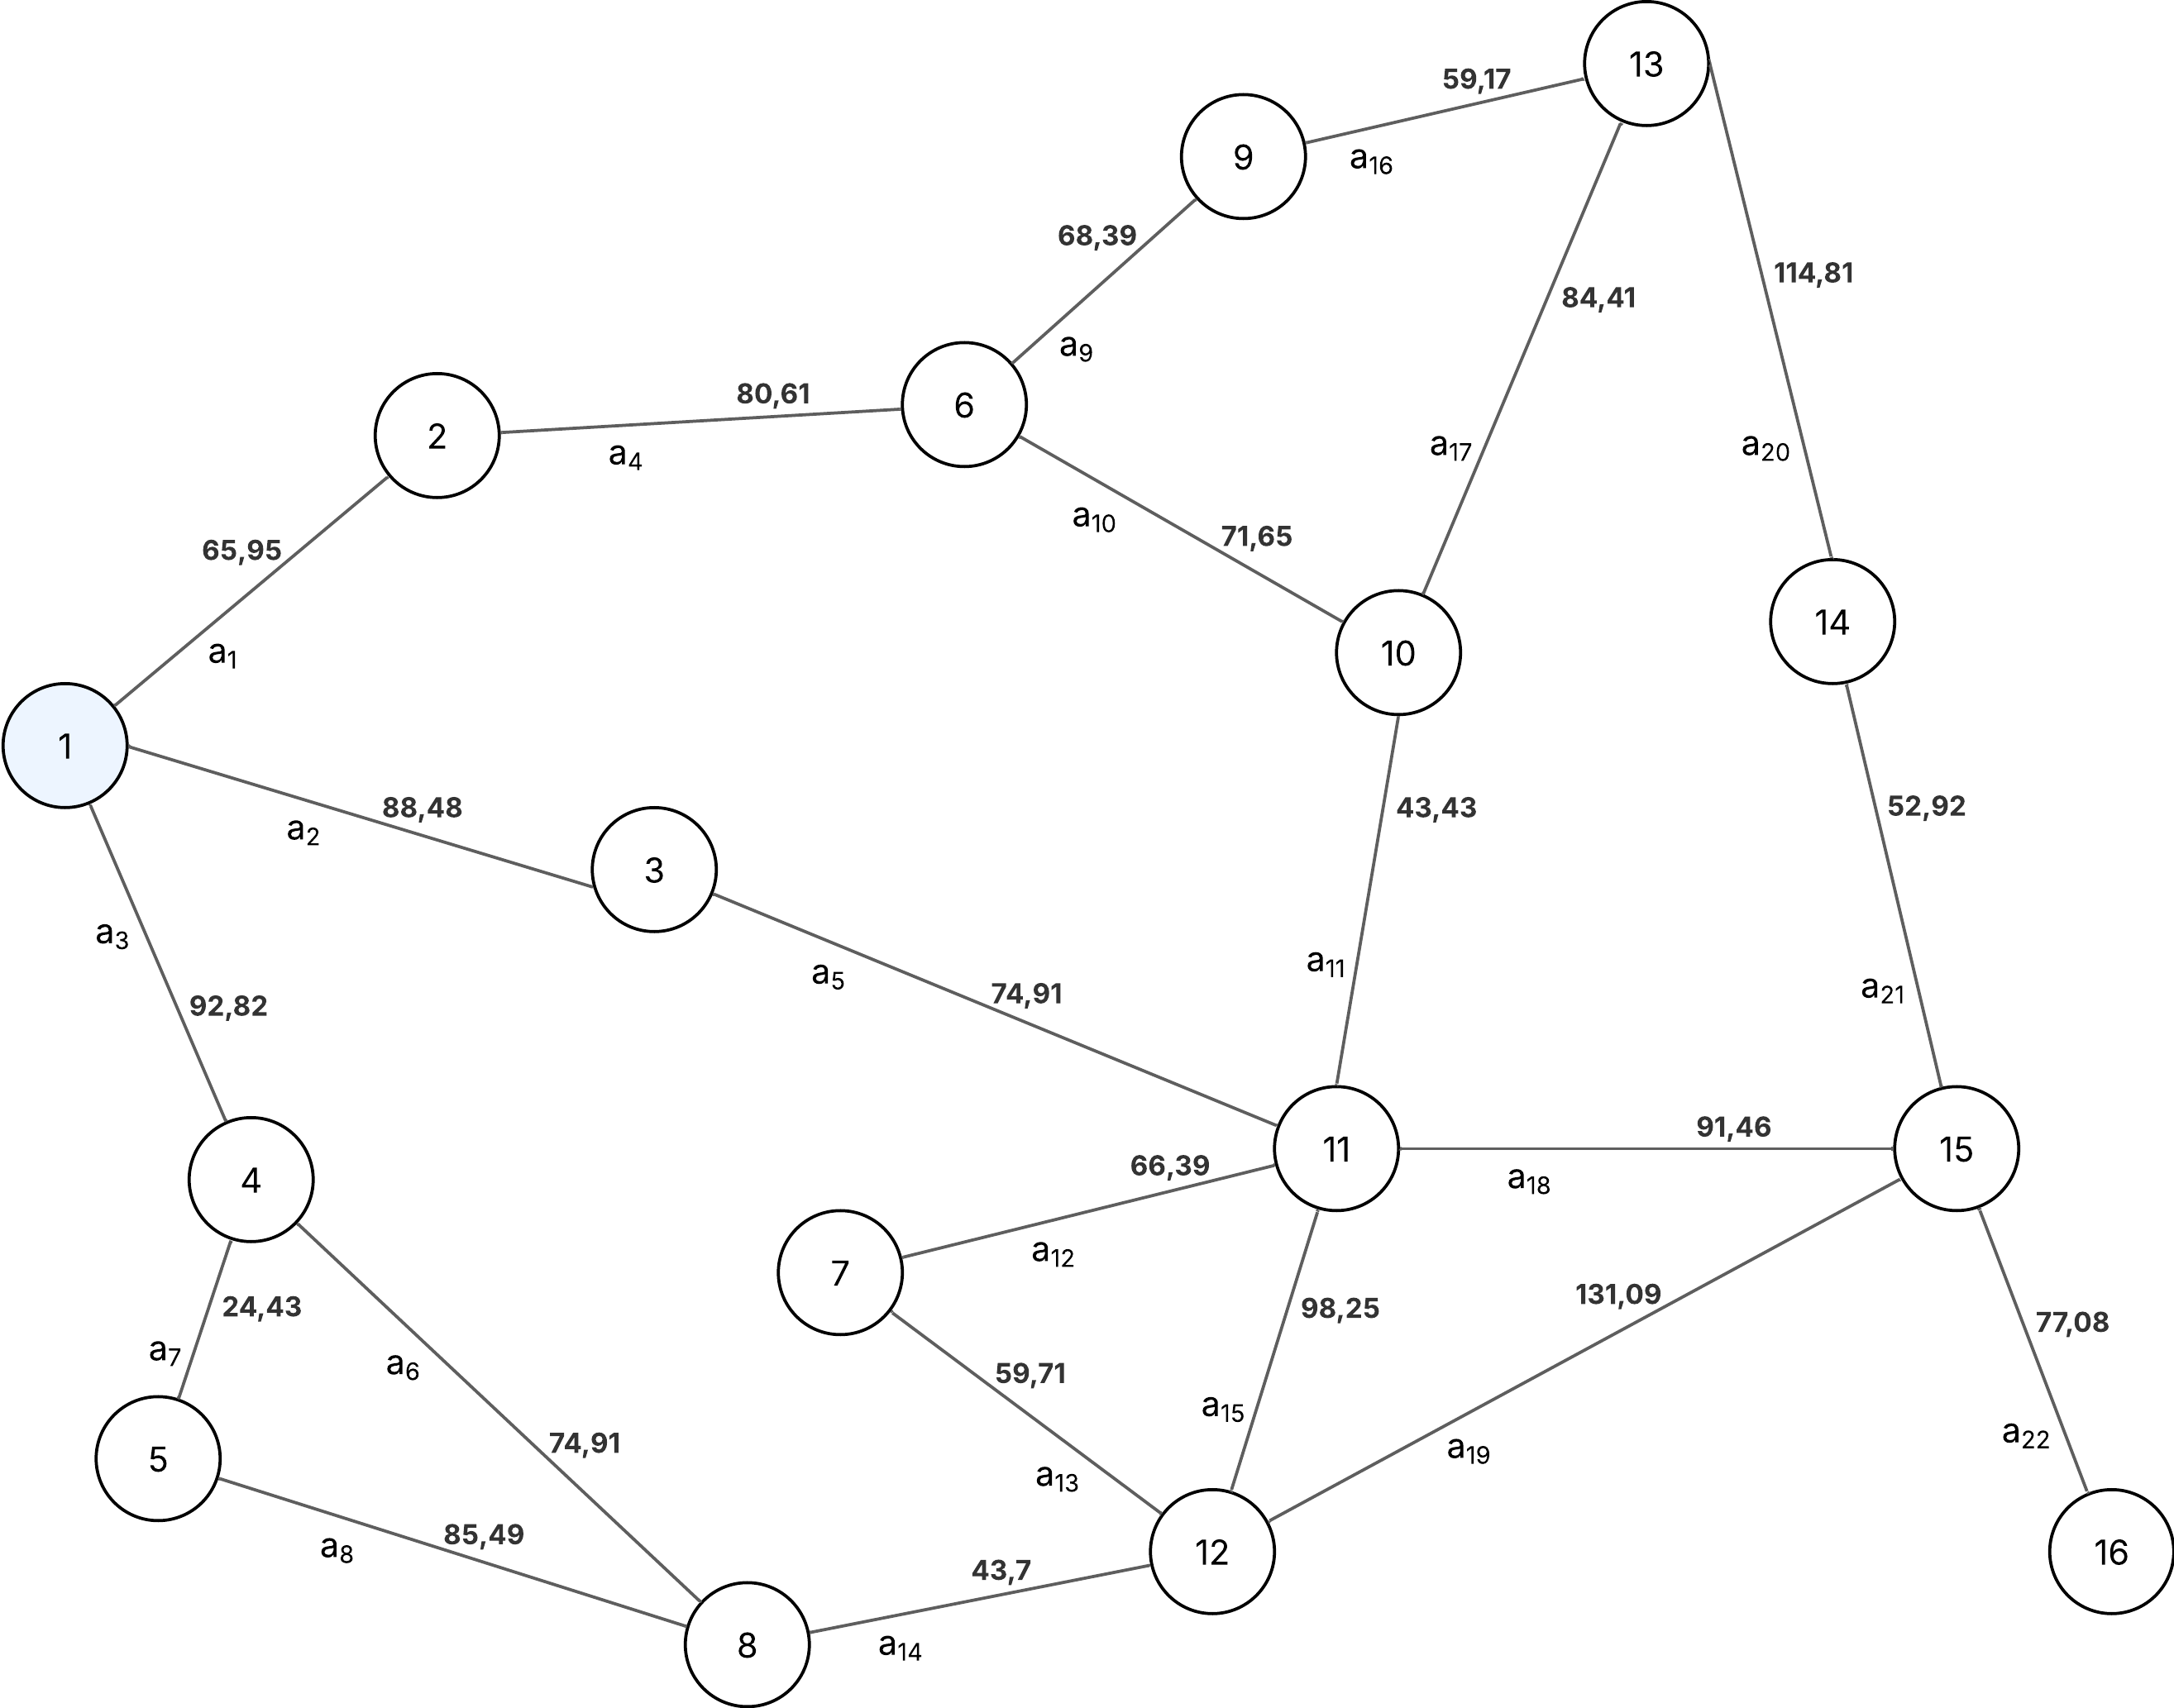
\includegraphics[width=1\textwidth,angle=0]{figuras/grafoGeometrico.png}%% Dimensões e localização
	\centering{Fonte: Criação própria}%% Fonte
\end{figure}


\section{Matriz de Adjacência}\label{sec:matriz}

A matriz de Adjacência do nosso problema é representada por (Equação \ref{eq:matrizAdj})


\begin{equation} \label{eq:matrizAdj}
	\begin{bmatrix}
		0 & 1 & 1 & 1 & 0 & 0 & 0 & 0 & 0 & 0 & 0 & 0 & 0 & 0 & 0 & 0 \\% 1
		1 & 0 & 0 & 0 & 0 & 1 & 0 & 0 & 0 & 0 & 0 & 0 & 0 & 0 & 0 & 0 \\% 2
		1 & 0 & 0 & 0 & 0 & 0 & 0 & 0 & 0 & 0 & 1 & 0 & 0 & 0 & 0 & 0 \\% 3
		1 & 0 & 0 & 0 & 1 & 0 & 0 & 1 & 0 & 0 & 0 & 0 & 0 & 0 & 0 & 0 \\% 4
		0 & 0 & 0 & 1 & 0 & 0 & 0 & 1 & 0 & 0 & 0 & 0 & 0 & 0 & 0 & 0 \\% 5
		0 & 1 & 0 & 0 & 0 & 0 & 0 & 0 & 1 & 1 & 0 & 0 & 0 & 0 & 0 & 0 \\% 6
		0 & 0 & 0 & 0 & 0 & 0 & 0 & 0 & 0 & 0 & 1 & 1 & 0 & 0 & 0 & 0 \\% 7
		0 & 0 & 0 & 1 & 1 & 0 & 0 & 0 & 0 & 0 & 0 & 1 & 0 & 0 & 0 & 0 \\% 8
		0 & 0 & 0 & 0 & 0 & 1 & 0 & 0 & 0 & 0 & 0 & 0 & 1 & 0 & 0 & 0 \\% 9
		0 & 0 & 0 & 0 & 0 & 1 & 0 & 0 & 0 & 0 & 1 & 0 & 1 & 0 & 0 & 0 \\% 10
		0 & 0 & 1 & 0 & 0 & 0 & 1 & 0 & 0 & 1 & 0 & 1 & 0 & 0 & 1 & 0 \\% 11
		0 & 0 & 0 & 0 & 0 & 0 & 1 & 1 & 0 & 0 & 1 & 0 & 0 & 0 & 1 & 0 \\% 12
		0 & 0 & 0 & 0 & 0 & 0 & 0 & 0 & 1 & 1 & 0 & 0 & 0 & 1 & 0 & 0 \\% 13
		0 & 0 & 0 & 0 & 0 & 0 & 0 & 0 & 0 & 0 & 0 & 0 & 1 & 0 & 1 & 0 \\% 14
		0 & 0 & 0 & 0 & 0 & 0 & 0 & 0 & 0 & 0 & 1 & 1 & 0 & 1 & 0 & 1 \\% 15
		0 & 0 & 0 & 0 & 0 & 0 & 0 & 0 & 0 & 0 & 0 & 0 & 0 & 0 & 1 & 0 % 16
	\end{bmatrix}
\end{equation}



\section{Lista de Adjacência}\label{sec:lista}

A lista de Adjacência do nosso problema é representada na figura \ref{fig:grafListaAdj}:

\begin{figure} [H]
	\centering
	\caption{Representação Lista de Adjacência}%% Legenda
	\label{fig:grafListaAdj}%% Rótulo
	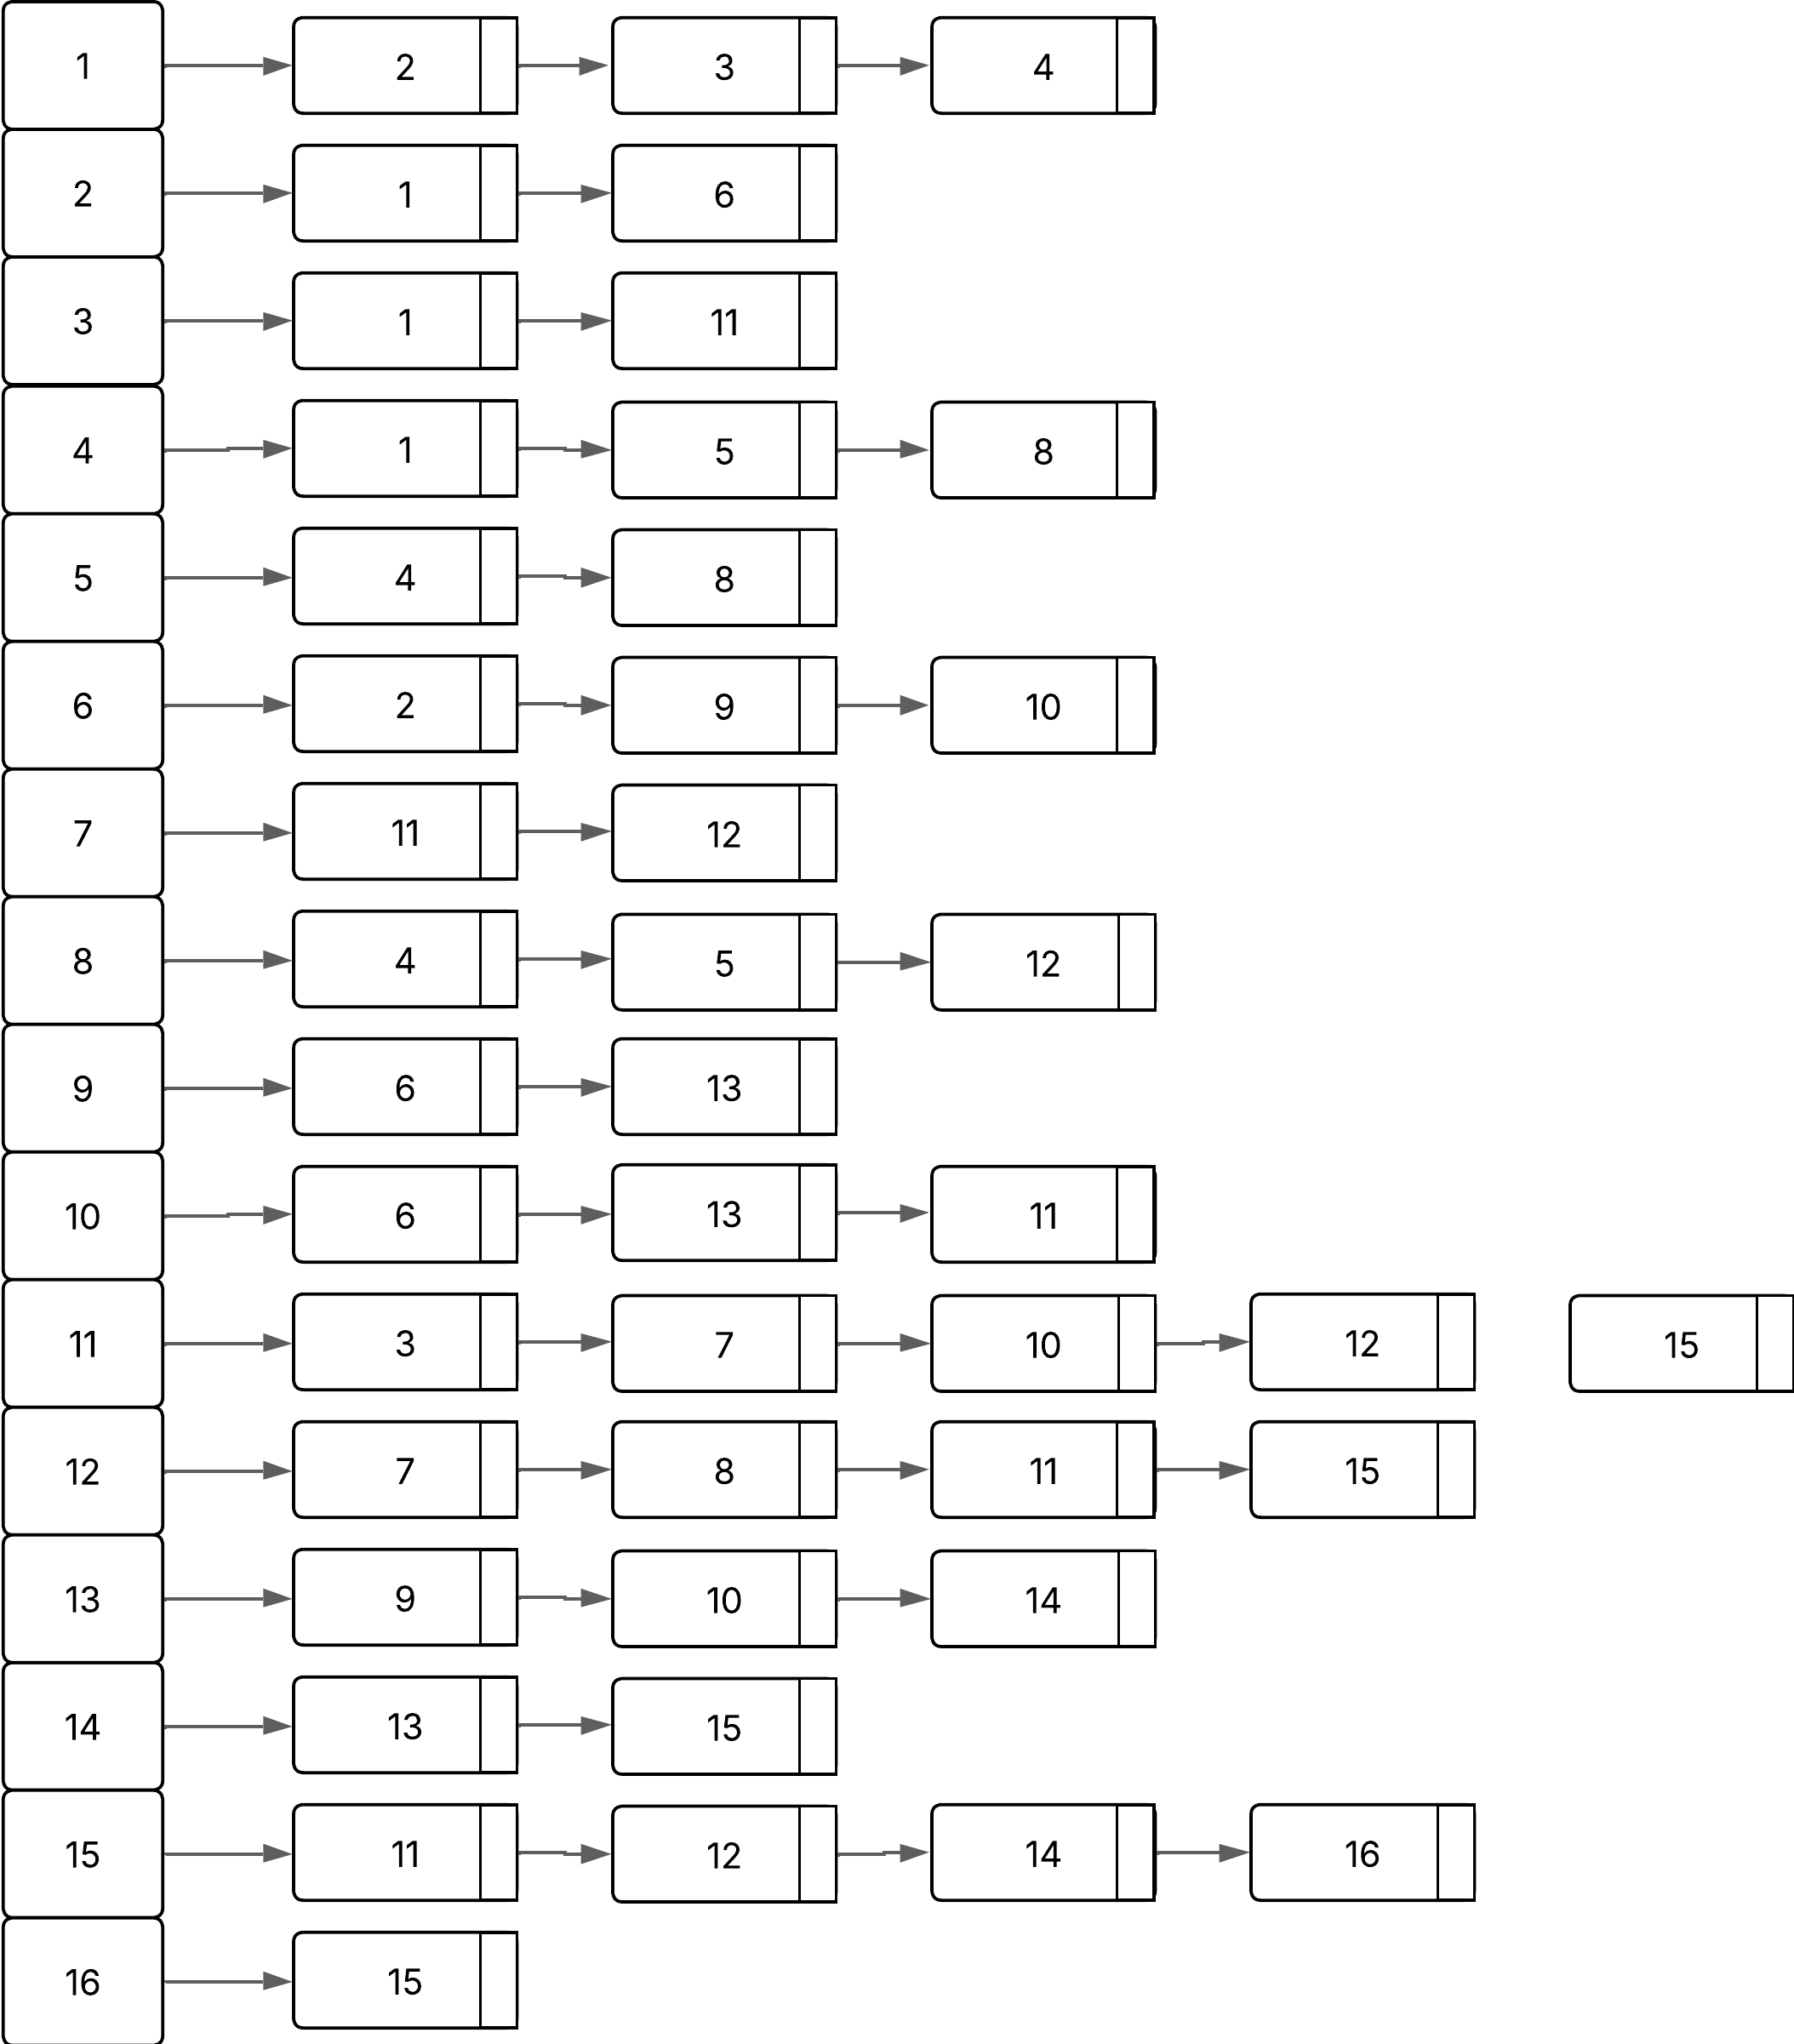
\includegraphics[width=1\linewidth,angle=0]{figuras/grafoListaAdj.png}%% Dimensões e localização
	\\
	\centering{Fonte: Criação própria}%% Fonte
\end{figure}

\section{Matriz de Incidência}\label{sec:incidencia}

A matriz de Incidência do nosso problema é (Equação \ref{eq:matrizInc}):

\begin{equation}
	\begin{bmatrix} \label{eq:matrizInc}
		1 & 1 & 1 & 0 & 0 & 0 & 0 & 0 & 0 & 0 & 0 & 0 & 0 & 0 & 0 & 0 & 0 & 0 & 0 & 0 & 0 & 0 \\% 1
		1 & 0 & 0 & 1 & 0 & 0 & 0 & 0 & 0 & 0 & 0 & 0 & 0 & 0 & 0 & 0 & 0 & 0 & 0 & 0 & 0 & 0 \\% 2
		0 & 1 & 0 & 0 & 1 & 0 & 0 & 0 & 0 & 0 & 0 & 0 & 0 & 0 & 0 & 0 & 0 & 0 & 0 & 0 & 0 & 0 \\% 3
		0 & 0 & 1 & 0 & 0 & 1 & 1 & 0 & 0 & 0 & 0 & 0 & 0 & 0 & 0 & 0 & 0 & 0 & 0 & 0 & 0 & 0 \\% 4
		0 & 0 & 0 & 0 & 0 & 0 & 1 & 1 & 0 & 0 & 0 & 0 & 0 & 0 & 0 & 0 & 0 & 0 & 0 & 0 & 0 & 0 \\% 5
		0 & 0 & 0 & 1 & 0 & 0 & 0 & 0 & 1 & 1 & 0 & 0 & 0 & 0 & 0 & 0 & 0 & 0 & 0 & 0 & 0 & 0 \\% 6
		0 & 0 & 0 & 0 & 0 & 1 & 0 & 0 & 0 & 0 & 0 & 1 & 1 & 0 & 0 & 0 & 0 & 0 & 0 & 0 & 0 & 0 \\% 7
		0 & 0 & 0 & 0 & 0 & 0 & 0 & 1 & 0 & 0 & 0 & 0 & 0 & 1 & 0 & 0 & 0 & 0 & 0 & 0 & 0 & 0 \\% 8
		0 & 0 & 0 & 0 & 0 & 0 & 0 & 0 & 1 & 0 & 0 & 0 & 0 & 0 & 0 & 1 & 0 & 0 & 0 & 0 & 0 & 0 \\% 9
		0 & 0 & 0 & 0 & 0 & 0 & 0 & 0 & 0 & 1 & 1 & 0 & 0 & 0 & 0 & 0 & 1 & 0 & 0 & 0 & 0 & 0 \\% 10
		0 & 0 & 0 & 0 & 1 & 0 & 0 & 0 & 0 & 0 & 1 & 1 & 0 & 0 & 1 & 0 & 0 & 1 & 0 & 0 & 0 & 0 \\% 11
		0 & 0 & 0 & 0 & 0 & 0 & 0 & 0 & 0 & 0 & 0 & 0 & 1 & 1 & 1 & 0 & 0 & 0 & 1 & 0 & 0 & 0 \\% 12
		0 & 0 & 0 & 0 & 0 & 0 & 0 & 0 & 0 & 0 & 0 & 0 & 0 & 0 & 0 & 1 & 1 & 0 & 0 & 1 & 0 & 0 \\% 13
		0 & 0 & 0 & 0 & 0 & 0 & 0 & 0 & 0 & 0 & 0 & 0 & 0 & 0 & 0 & 0 & 0 & 0 & 0 & 1 & 1 & 0 \\% 14
		0 & 0 & 0 & 0 & 0 & 0 & 0 & 0 & 0 & 0 & 0 & 0 & 0 & 0 & 0 & 0 & 0 & 1 & 1 & 0 & 1 & 1 \\% 15
		0 & 0 & 0 & 0 & 0 & 0 & 0 & 0 & 0 & 0 & 0 & 0 & 0 & 0 & 0 & 0 & 0 & 0 & 0 & 0 & 0 & 1 % 16
	\end{bmatrix}
\end{equation}


\section{Considerações de Eficiência}\label{sec:eficienciaRepresentacao}
Para o nosso grafo, acredita-se que, a representação com melhor eficiência, ou seja, menor custo computacional é a lista de adjacências, por termos múltiplos vértices e arestas, e por seu O(|V| + |X|) = O(38). Calculo de todas as representações:
\begin{itemize}
	\item Matriz de Adjacências:\\
	      \begin{equation}
		      O(V^2) = O(16^2) = O(256)
	      \end{equation}
	\item Lista de Adjacências: \\
	      \begin{equation}
		      O(|V| + |X|) = O(16 + 22) = O(38)
	      \end{equation}
	\item Matriz de Incidência:
	      \begin{equation}
		      O(V\times X) = O(16\times22) = O(352)
	      \end{equation}
\end{itemize}

\chapter{Definições em um Grafo }\label{cap:definicoesGrafo}

Como a estrutura de dados grafo é uma estrutura heterogenia, definições são necessárias para compreender partes ou o todo da estrutura. Na Seção \ref{sec:terminologias}, as principais terminologias, considerando o grafo representado graficamente na Figura  \ref{fig:grafGeometrico}, são apresentadas. Enquanto, na Seção \ref{sec:tiposGrafos}, todos os tipos os quais o grafo estudado contempla são apresentados.

\section{Terminologias}\label{sec:terminologias}

A terminologia se inicia com a definição da orientação e adjacências do grafo.
O grafo em questão, demonstrado na figura, não é orientado, tendo em vista sua representação (sem setas de direcionamento), bem como a sua ideia de representar apenas avenidas e/ou rodovias, que são sempre duas mãos.
A adjacência se baseia em 5 fatores: adjacência de vértices, arestas, incidência, paralelismo e laço.

A adjacência de vértices é entendida quando dois vértices são ligados entre si com uma ou mais arestas.
No caso do grafo não direcionado, dois vértices adjacentes são sempre adjacentes entre si.
Exemplo: $V_6$ é adjacente a $V_9$, da mesma maneira $V_9$ é adjacente a $V_6$.

A adjacência de arestas é parecida, mas dessa vez, arestas são adjacentes quando compartilham um mesmo vértice.
Exemplo: $A_{20}$ é adjacente a $A_{17}$, pois compartilham o mesmo vértice $V_{13}$.

As incidências são a notação para uma aresta que liga dois vértices.
Exemplo: $A_{5}$ é incidente em $V_3$ e $V_{11}$ ao mesmo tempo devido ao grafo ser não orientado.

Arestas paralelas são duas arestas que ligam o mesmo par de vértices.
No grafo em questão não existem arestas paralelas.

Por fim, o laço é uma aresta que liga o vértice nele mesmo.
No grafo em questão não existe laço, tendo em vista que as arestas representam avenidas que vão de uma cidade e/ou distrito até outra, o que torna impensável uma aresta que liga um vértice a si próprio.

Terminando de falar das adjacências, tem-se a aplicação multívoca $\Gamma$, que representa os sucessores de um vértice, ou de forma mais simples, os vértices que são ligados ao vértice em questão.

\[
	\begin{alignedat}{2}
		\Gamma(1) & = (2,3,4)  & \quad \Gamma(9)  & = (6,13)         \\
		\Gamma(2) & = (1,6)    & \quad \Gamma(10) & = (6,11,13)      \\
		\Gamma(3) & = (1,11)   & \quad \Gamma(11) & = (3,7,10,12,15) \\
		\Gamma(4) & = (1,5,8)  & \quad \Gamma(12) & = (7,8,11,15)    \\
		\Gamma(5) & = (4,8)    & \quad \Gamma(13) & = (9,10,14)      \\
		\Gamma(6) & = (2,9,10) & \quad \Gamma(14) & = (13,15)        \\
		\Gamma(7) & = (11,12)  & \quad \Gamma(15) & = (11,14,16)     \\
		\Gamma(8) & = (4,5,12) & \quad \Gamma(16) & = (15)
	\end{alignedat}
\]

Existe também a aplicação gama inversa, que seria para os vértices que se ligam em $V$ mas $V$ não se liga nos vértices.
No entanto, só é possível fazer essa aplicação em grafos direcionados, pois eles têm direcionamento.
Já no grafo não direcionado, toda aresta que vai, volta.

Junto da aplicação, é possível calcular o grau de cada vértice, que em um grafo não direcionado é basicamente o número de vértices ligados ao $V$ em questão (evidenciado na aplicação gama).
Em um grafo direcionado, o cálculo é basicamente o mesmo, só que somando também com a aplicação inversa.

\[
	\begin{aligned}
		V_1    & = 3, \
		V_2    & = 2     \\
		V_3    & = 2, \
		V_4    & = 3     \\
		V_5    & = 2, \
		V_6    & = 3     \\
		V_7    & = 2, \
		V_8    & = 3     \\
		V_9    & = 2, \
		V_{10} & = 3     \\
		V_{11} & = 5, \
		V_{12} & = 4     \\
		V_{13} & = 3,\
		V_{14} & = 2     \\
		V_{15} & = 3,\
		V_{16} & = 1
	\end{aligned}
\]

\[
	\text{Ordem do grafo} = 16 \qquad \text{Tamanho do grafo} = 22
\]

Continuando na ligação entre os vértices, podemos gerar conjuntos de ligações chamadas de cadeia e ciclo.
No caso do grafo não direcionado, uma cadeia é um conjunto de ligações no grafo que levam de um $V_X$ para um $V_Y$.

Exemplo de cadeia:
\[
	C(V_1 \rightarrow V_{16}) = ((V_1,V_4),(V_4,V_8),(V_8,V_{12}),(V_{12},V_{15}),(V_{15},V_{16})).
\]

E o ciclo é uma cadeia, mas o último vértice visitado é o mesmo que se inicia, ou seja, um conjunto de ligações que levam de $V_X$ para $V_X$.

Exemplo de ciclo:
\[
	C(V_6 \rightarrow V_6) = ((V_6,V_9),(V_9,V_{13}),(V_{13},V_{10}),(V_{10},V_6)).
\]

Podemos também classificar as cadeias e ciclos em alguns tipos, dentre eles Elementar e Simples.
No caso, a cadeia/ciclo elementar é quando todos os vértices são distintos, ou seja, a cadeia ou ciclo passa pelo vértice apenas uma vez.
Já a cadeia/ciclo simples é quando a cadeia passa por uma aresta apenas uma vez.

Exemplos de cadeia/ciclo elementar:
\[
	C(V_4 \rightarrow V_4) = ((V_4,V_5),(V_5,V_8),(V_8,V_4))
\]
\[
	C(V_7 \rightarrow V_7) = ((V_7,V_{12}),(V_{12},V_{15}),(V_{15},V_{11}),(V_{11},V_7))
\]

Também é possível classificar em cadeia/ciclo euleriano e hamiltoniano.
Euleriano é quando todas as arestas são percorridas exatamente uma vez, e hamiltoniano é quando todos os vértices são percorridos exatamente uma vez.

No grafo utilizado não existe possibilidade de uma cadeia/ciclo desses dois tipos, pois qualquer caminho teria de passar por alguma aresta ou vértice mais de uma vez ou deixar alguma aresta/vértice de fora do caminho.


\section{Tipos de Grafos}\label{sec:tiposGrafos}
\textit{\textbf{Grafo nulo:}} um grafo em que seu conjunto de vértices e seu conjunto de arestas são vazios. \par
\textit{\textbf{Grafo Trivial ou Singleton:}} grafo com apenas um vértice.
\begin{figure} [H]
	\centering
	\caption{Singleton}%% Legenda
	\label{fig:singleton}%% Rótulo
	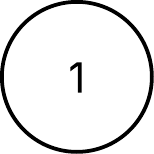
\includegraphics[width=0.1\linewidth,angle=0]{figuras/tiposgrafos/singleton.png}%% Dimensões e localização
	\\
	\centering{Fonte: Criação própria}%% Fonte
\end{figure}
\par
\textit{\textbf{Grafo Vazio:}} Grafo que não possui nenhuma aresta, apenas vértices.
\begin{figure} [H]
	\centering
	\caption{Grafo Vazio}%% Legenda
	\label{fig:grafVazio}%% Rótulo
	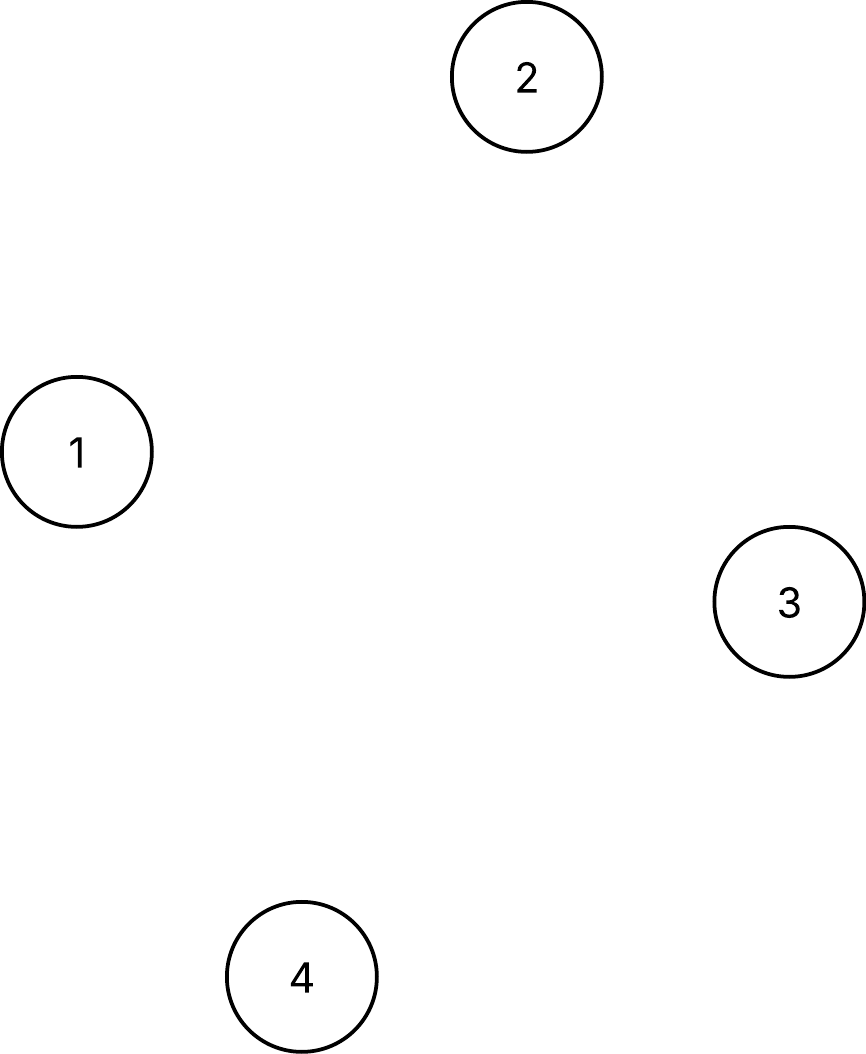
\includegraphics[width=0.5\linewidth,angle=0]{figuras/tiposgrafos/grafVazio.png}%% Dimensões e localização
	\\
	\centering{Fonte: Criação própria}%% Fonte
\end{figure}
\textit{\textbf{Buquê:}} um vértice com n laços.
\begin{figure} [H]
	\centering
	\caption{Buquê}%% Legenda
	\label{fig:buquê}%% Rótulo
	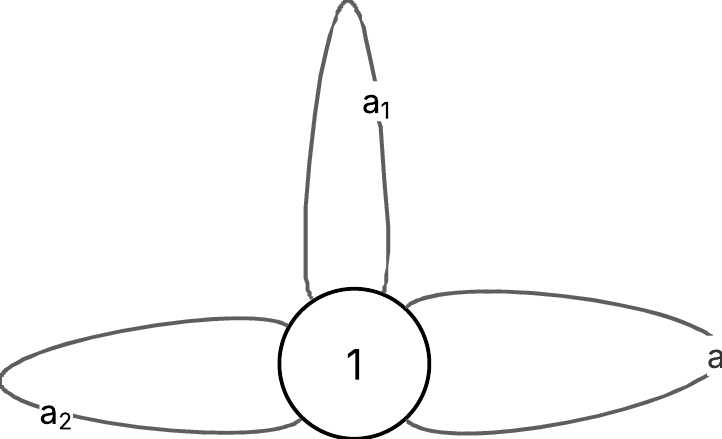
\includegraphics[width=0.5\linewidth,angle=0]{figuras/tiposgrafos/buque.png}%% Dimensões e localização
	\\
	\centering{Fonte: Criação própria}%% Fonte
\end{figure}
\textit{\textbf{Pseudografo:}} contém pelo menos um laço. \\
\begin{figure} [H]
	\centering
	\caption{Pseudografo}%% Legenda
	\label{fig:pseudografo}%% Rótulo
	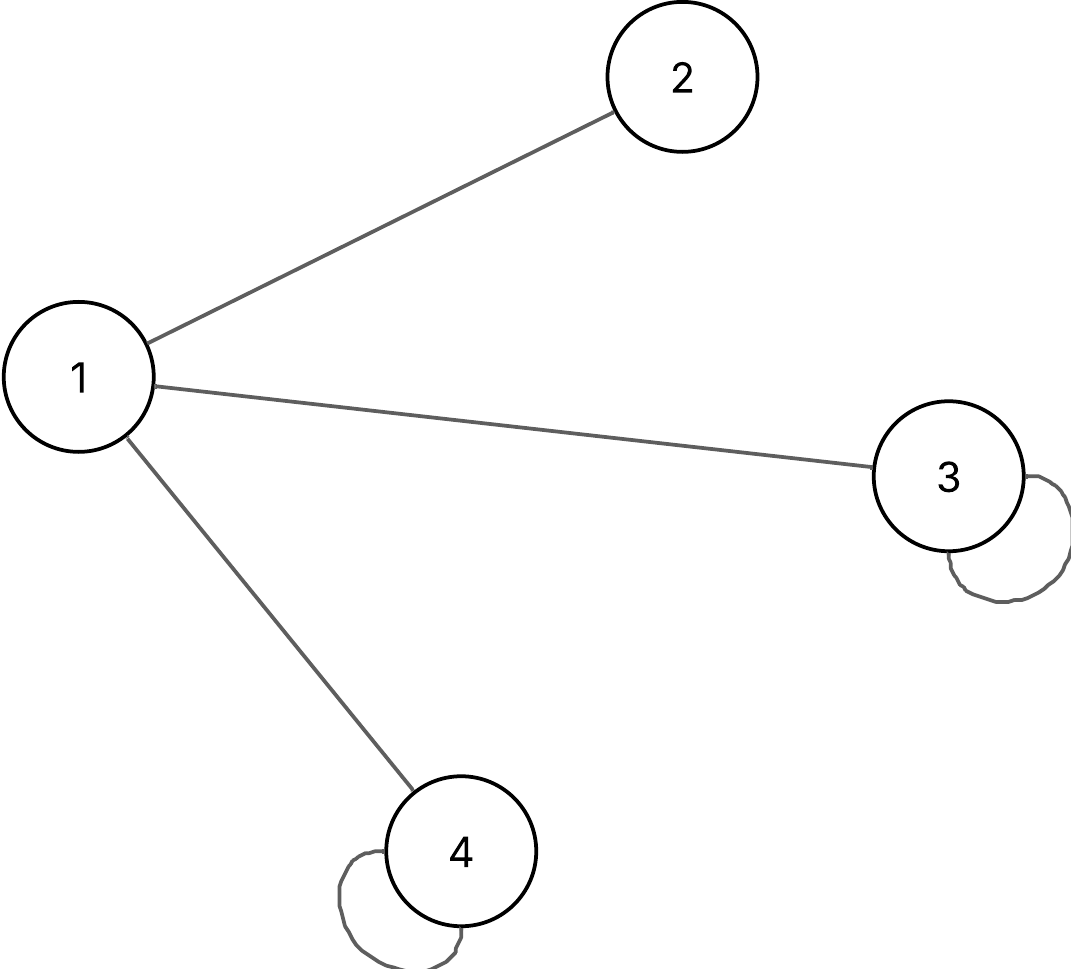
\includegraphics[width=0.5\linewidth,angle=0]{figuras/tiposgrafos/pseudografo.png}%% Dimensões e localização
	\\
	\centering{Fonte: Criação própria}%% Fonte
\end{figure}
\textit{\textbf{Grafo Reflexivo:}} Pseudografo em que cada vértice possui um laço associado.\\
\begin{figure} [H]
	\centering
	\caption{Grafo Reflexivo}%% Legenda
	\label{fig:grafReflex}%% Rótulo
	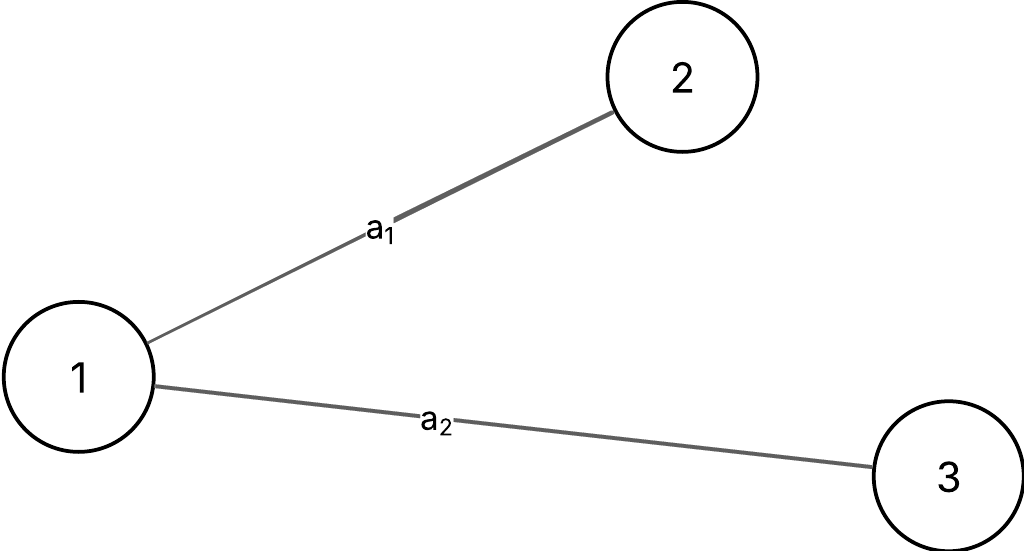
\includegraphics[width=0.5\linewidth,angle=0]{figuras/tiposgrafos/grafReflex.png}%% Dimensões e localização
	\\
	\centering{Fonte: Criação própria}%% Fonte
\end{figure}
\textit{\textbf{Multigrafo:}} Um grafo não orientado sem laços e possui no mínimo duas arestas paralelas. \\
\begin{figure} [H]
	\centering
	\caption{Multigrafo}%% Legenda
	\label{fig:multigraf}%% Rótulo
	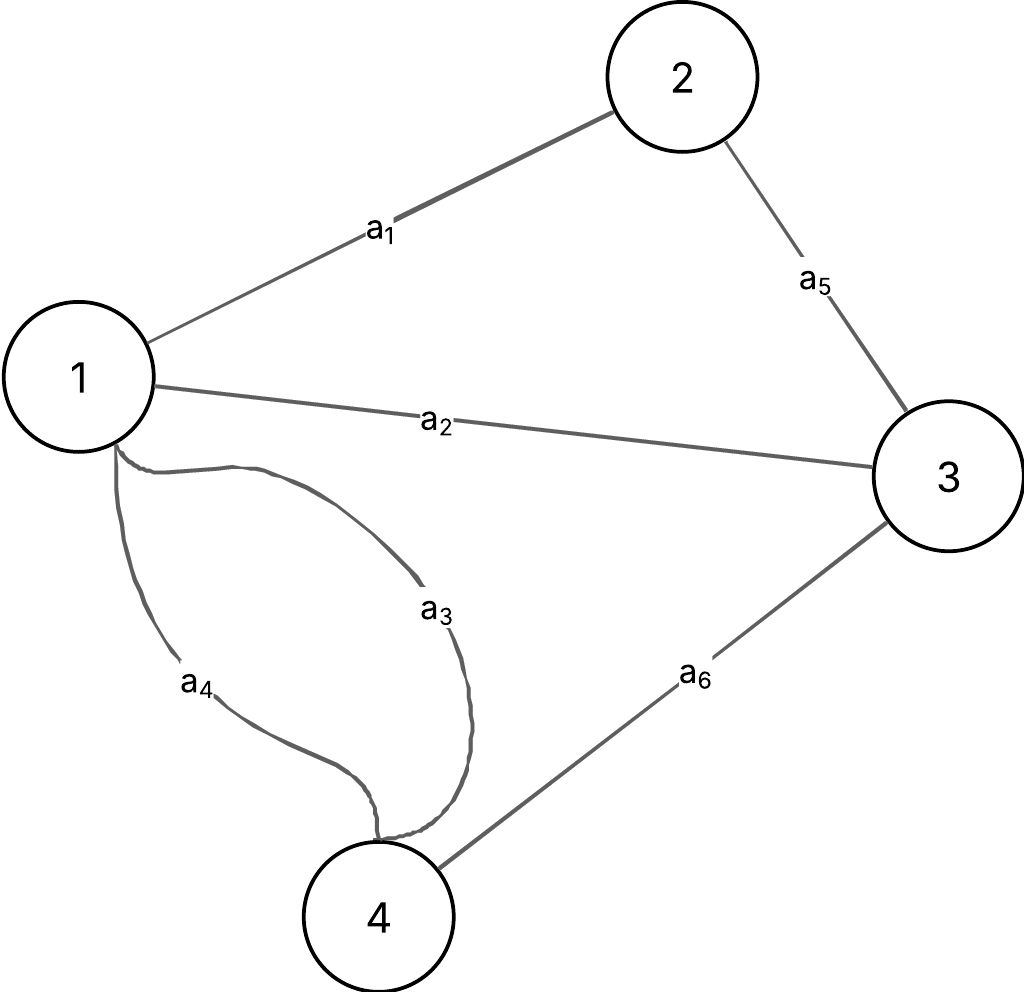
\includegraphics[width=0.5\linewidth,angle=0]{figuras/tiposgrafos/multigrafo.png}%% Dimensões e localização
	\\
	\centering{Fonte: Criação própria}%% Fonte
\end{figure}
\textit{\textbf{Multigrafo Direcionado:}} Um grafo orientado que possui laços e arestas paralelas. \\
\begin{figure} [H]
	\centering
	\caption{Multigrafo Direcionado}%% Legenda
	\label{fig:multigrafDirec}%% Rótulo
	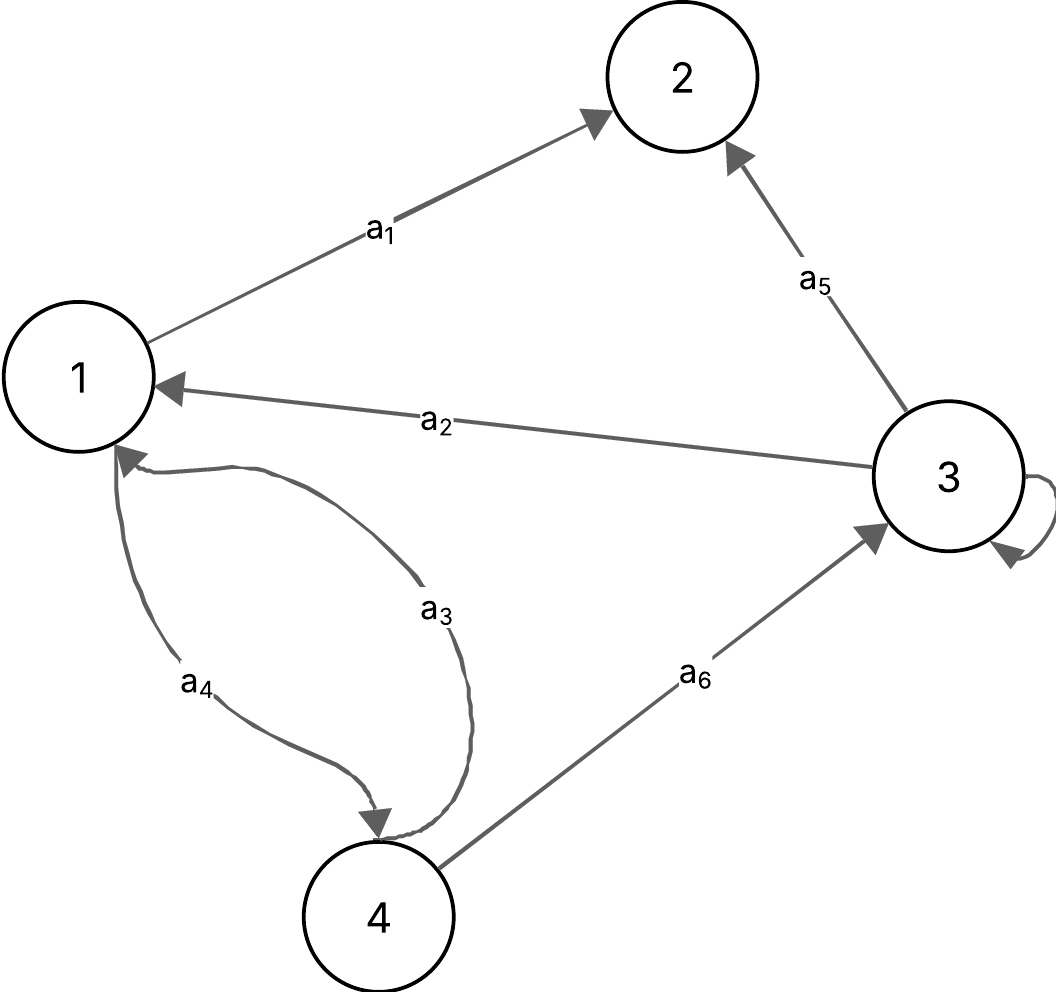
\includegraphics[width=0.5\linewidth,angle=0]{figuras/tiposgrafos/multigrafoDirec.png}%% Dimensões e localização
	\\
	\centering{Fonte: Criação própria}%% Fonte
\end{figure}
\textit{\textbf{Grafo Simples:}} Grafo sem laços e arestas paralelas.\\
\begin{figure} [H]
	\centering
	\caption{Grafo Simples}%% Legenda
	\label{fig:grafSimples}%% Rótulo
	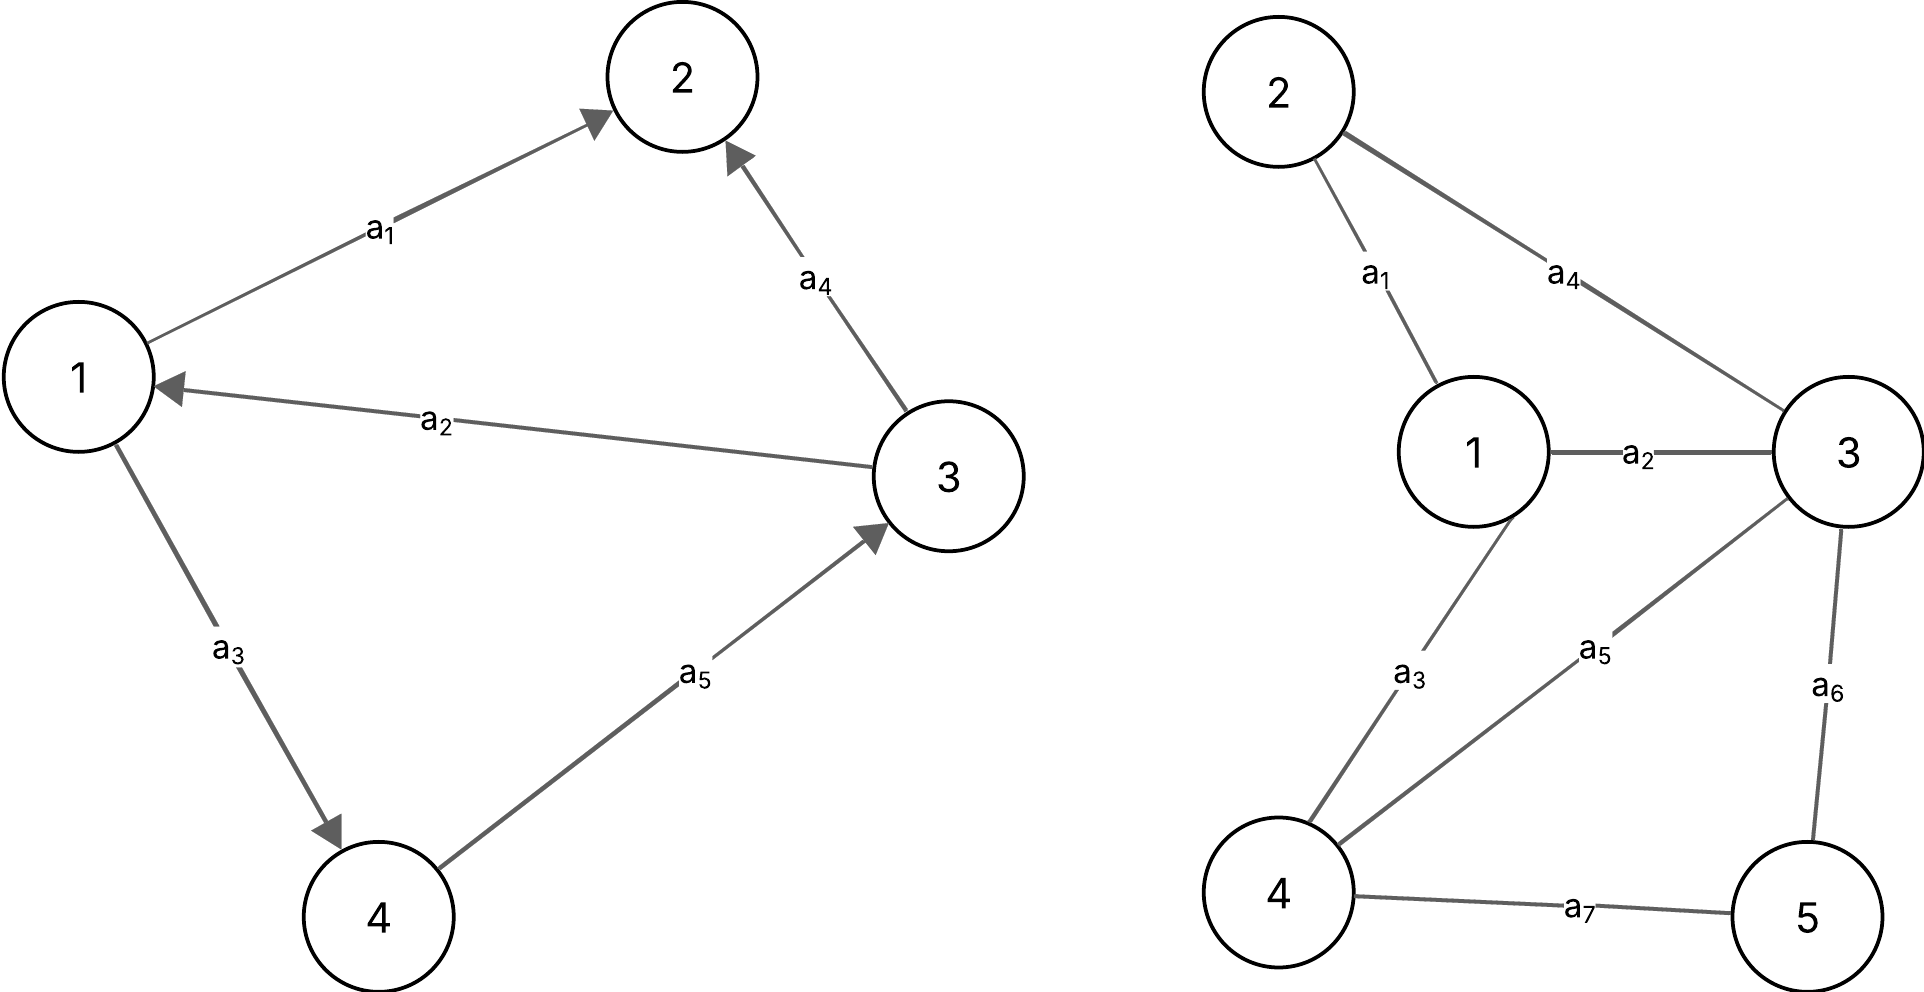
\includegraphics[width=0.7\linewidth,angle=0]{figuras/tiposgrafos/grafoSimples.png}%% Dimensões e localização
	\\
	\centering{Fonte: Criação própria}%% Fonte
\end{figure}
\textit{\textbf{Grafo acíclico:}} Grafo sem ciclos ou circuitos.\\
\begin{figure} [H]
	\centering
	\caption{Grafo Acíclico}%% Legenda
	\label{fig:grafAcicl}%% Rótulo
	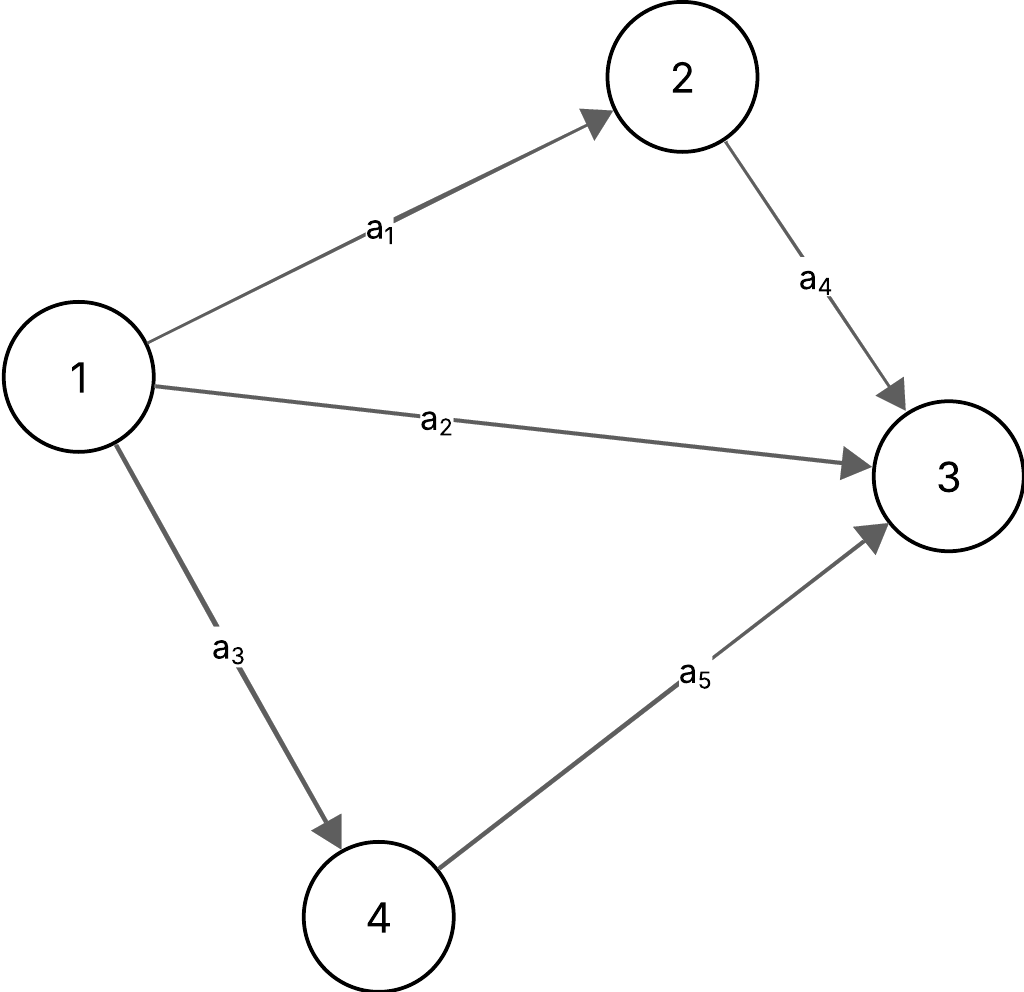
\includegraphics[width=0.5\linewidth,angle=0]{figuras/tiposgrafos/grafAcicl.png}%% Dimensões e localização
	\\
	\centering{Fonte: Criação própria}%% Fonte
\end{figure}
\textit{\textbf{Grafo ciclo:}} É um grafo simples não orientado regular, $ C_n $ com mais de dois vértices, onde forma um ciclo, ao partir de um vértice, é possível chegar nele novamente ao passar por todos os outros.\\
\begin{figure} [H]
	\centering
	\caption{Grafo Cíclico}%% Legenda
	\label{fig:grafCiclo}%% Rótulo
	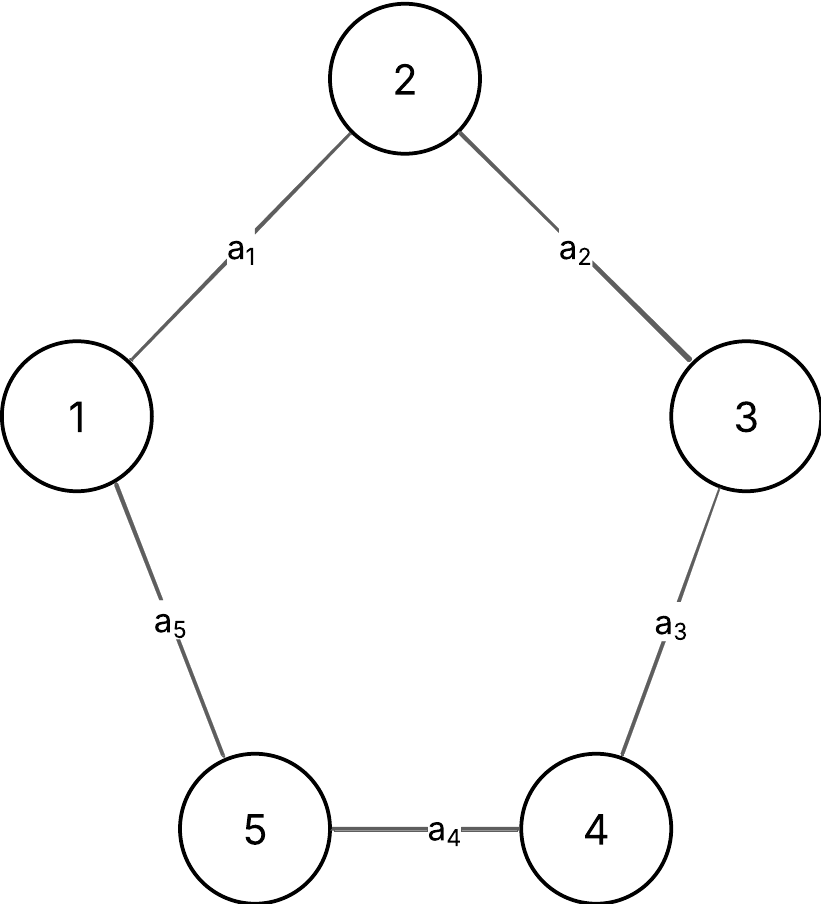
\includegraphics[width=0.5\linewidth,angle=0]{figuras/tiposgrafos/grafCiclo.png}%% Dimensões e localização
	\\
	\centering{Fonte: Criação própria}%% Fonte
\end{figure}
\textit{\textbf{Grafo roda:}} É um grafo não orientado simples, $ W_n $, com $ n+1 $ vértices, onde n é maior que 2, onde existe um vértice $ V_n+1 $ responsável por conectar os demais vértices entre si. \\
\begin{figure} [H]
	\centering
	\caption{Grafo Roda:}%% Legenda
	\label{fig:grafRoda}%% Rótulo
	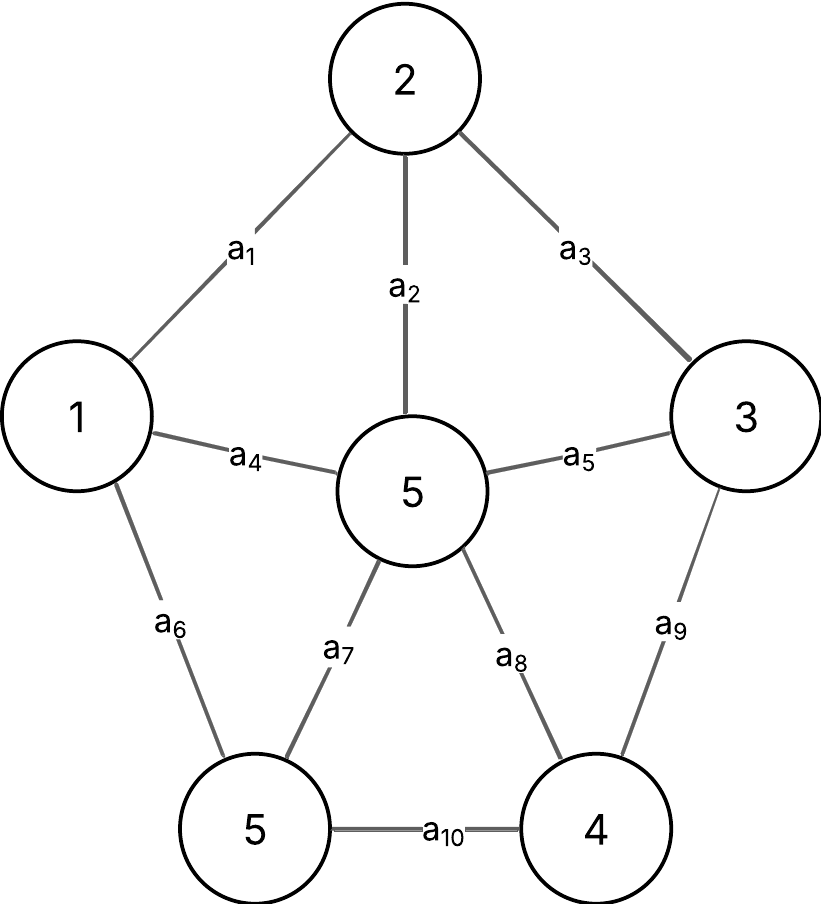
\includegraphics[width=0.5\linewidth,angle=0]{figuras/tiposgrafos/grafRoda.png}%% Dimensões e localização
	\\
	\centering{Fonte: Criação própria}%% Fonte
\end{figure}
\textit{\textbf{Grafo regular:}} Grafo, $ K_v $, onde todos os vértices possuem o mesmo grau, ou seja, mesmo número de vértices o que resulta em um grafo onde todos se conectam. \\
\begin{figure} [H]
	\centering
	\caption{Grafo Regular}%% Legenda
	\label{fig:grafRegular}%% Rótulo
	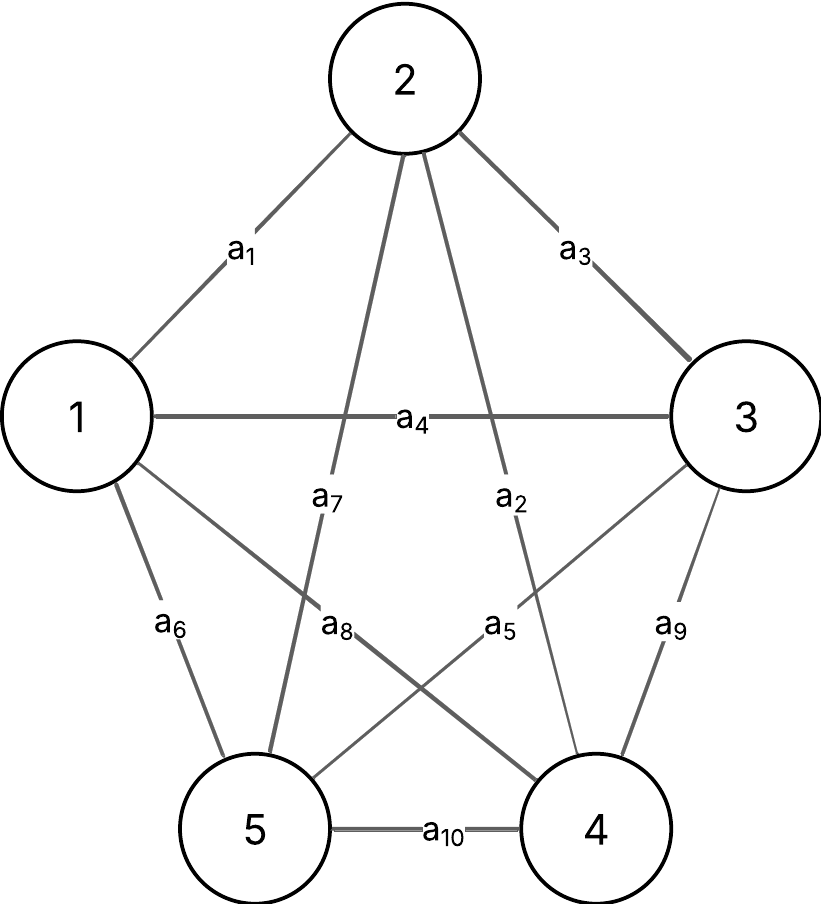
\includegraphics[width=0.5\linewidth,angle=0]{figuras/tiposgrafos/grafRegular.png}%% Dimensões e localização
	\\
	\centering{Fonte: Criação própria}%% Fonte
\end{figure}
\textit{\textbf{Grafo simétrico:}} Um grafo orientado, onde, para cada arco $ (v_i, v_j) \in X$ existe um arco $ (v_j,v_i)\in X $, em outras palavras, cada vértice possui um arco nos dois sentidos, formando simetria entre os arcos  \\
\begin{figure} [H]
	\centering
	\caption{Grafo Simétrico}%% Legenda
	\label{fig:grafSimetrico}%% Rótulo
	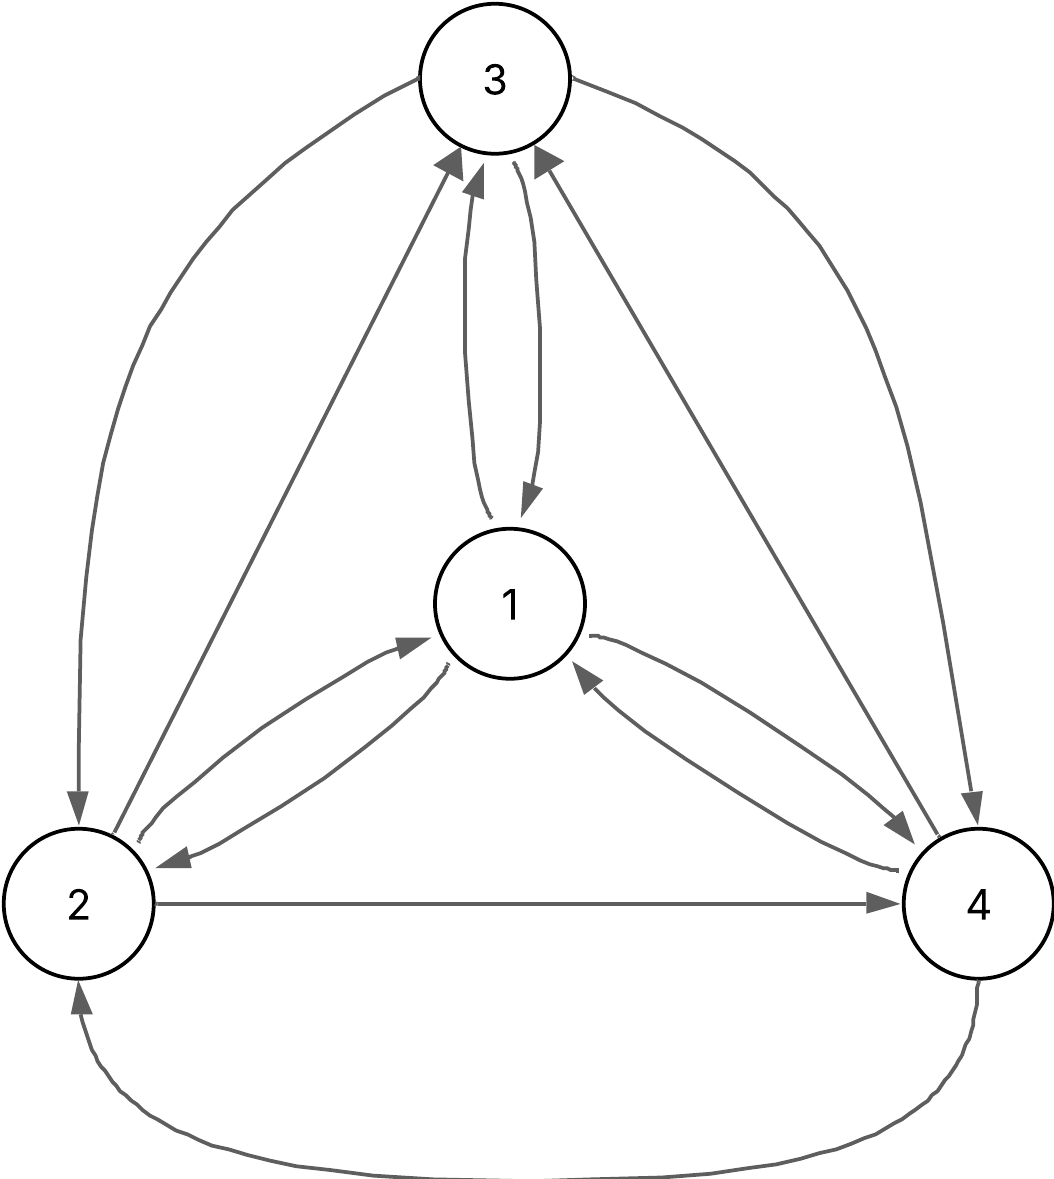
\includegraphics[width=0.5\linewidth,angle=0]{figuras/tiposgrafos/grafSimetrico.png}%% Dimensões e localização
	\\
	\centering{Fonte: Criação própria}%% Fonte
\end{figure}
\textit{\textbf{Grafo assimétrico:}}  Um grafo orientado, onde, para cada arco $ (v_i, v_j) \in X$ não existe um arco $ (v_j,v_i)\in X $, em outras palavras, cada vértice possui apenas um arco em apenas um sentido \\
\begin{figure} [H]
	\centering
	\caption{Grafo assimétrico}%% Legenda
	\label{fig:grafAssimet}%% Rótulo
	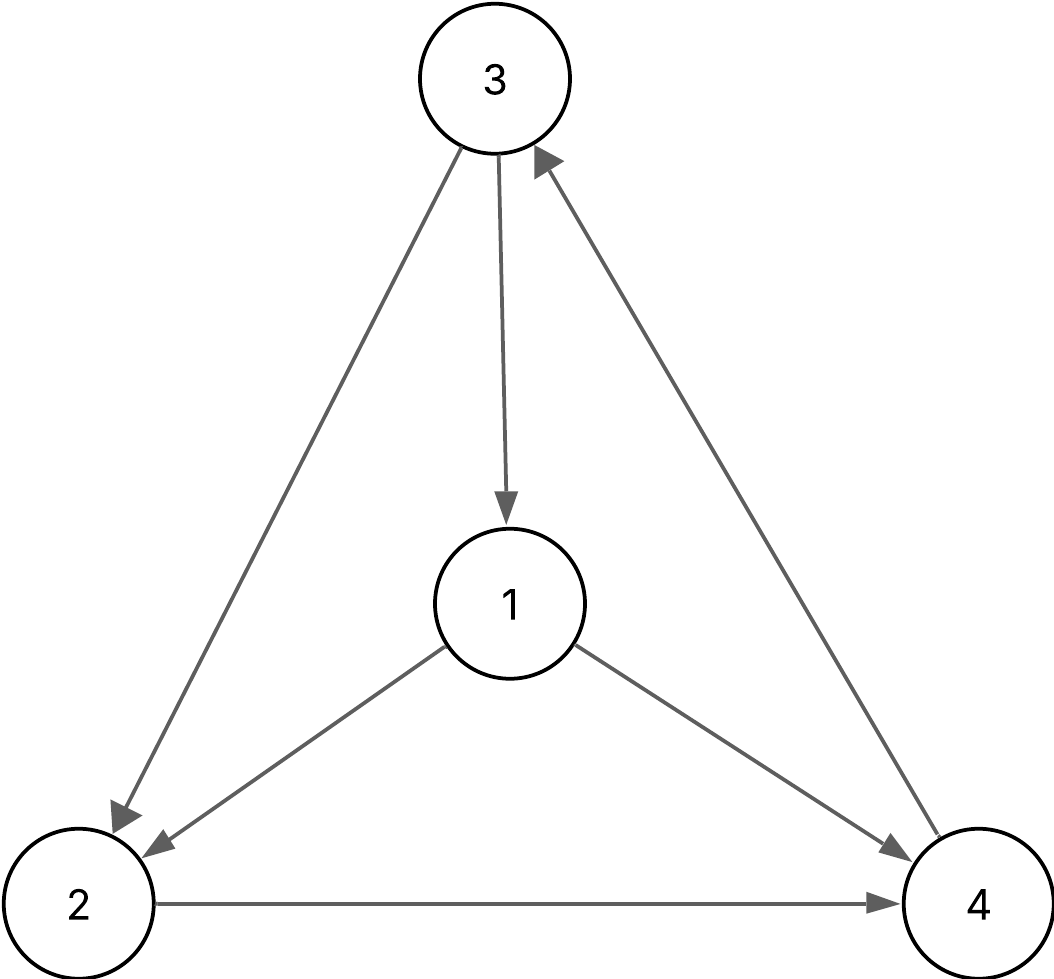
\includegraphics[width=0.5\linewidth,angle=0]{figuras/tiposgrafos/grafAssimet.png}%% Dimensões e localização
	\\
	\centering{Fonte: Criação própria}%% Fonte
\end{figure}
\textit{\textbf{Torneio:}} um grafo orientado que, para cada par $ (v_i, v_j) \in V $ com $ v_i \neq v_j $, $ (v_i, v_j)\in E $ é um arco ou $ (v_j, v_i) \in E $ é um arco, mas não ambos, fazendo com que exista apenas um arco entre dois vértices.
\begin{figure} [H]
	\centering
	\caption{Torneio}%% Legenda
	\label{fig:torneio}%% Rótulo
	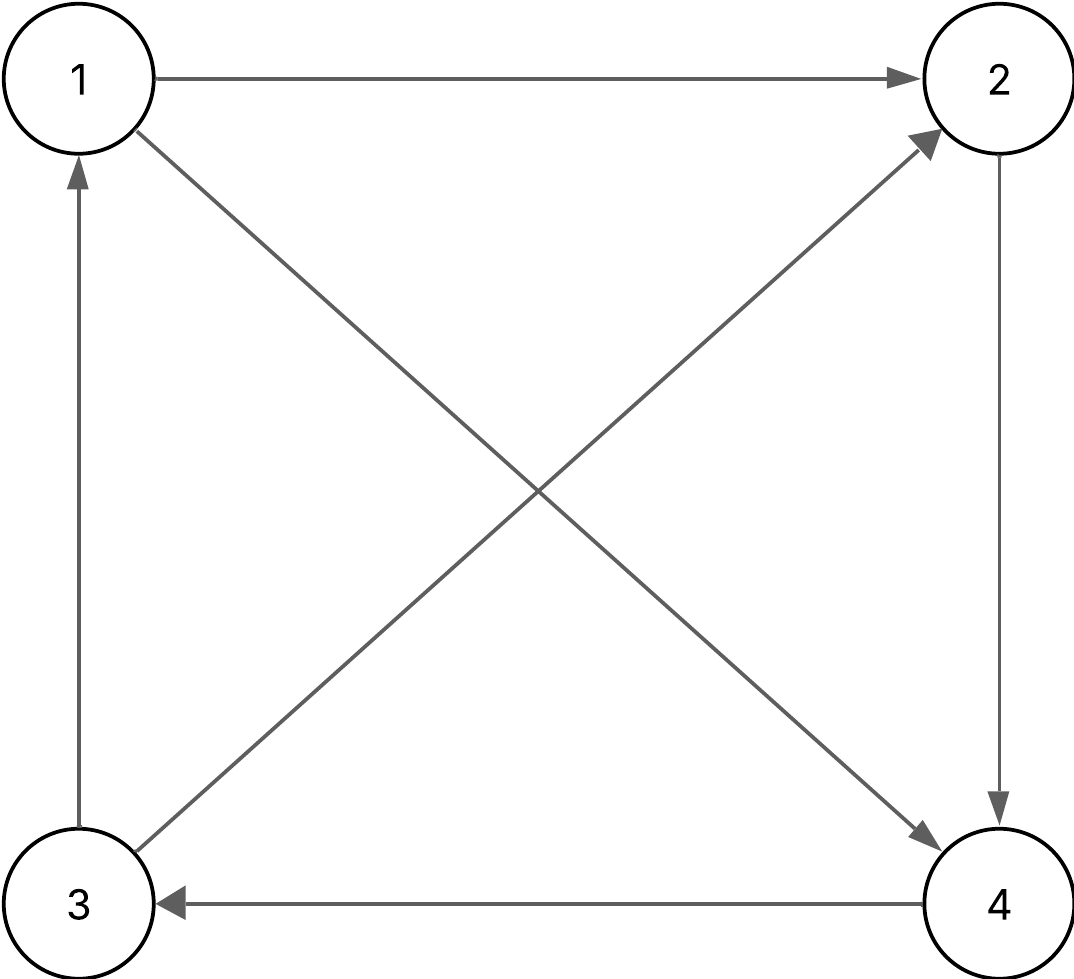
\includegraphics[width=0.5\linewidth,angle=0]{figuras/tiposgrafos/torneio.png}%% Dimensões e localização
	\\
	\centering{Fonte: Criação própria}%% Fonte
\end{figure}

% --- KAIQUE
\textit{\textbf{Completo:}} Grafo não direcionado simples onde todo par de vértices $v_i, v_j \in V$ é ligado por uma aresta, sendo essa $(v_i, v_j)$, sendo um grafo simples que contém o número maximo possível de arestas.

\begin{figure} [H]
	\centering
	\caption{Grafo Completo}%% Legenda
	\label{fig:completo}%% Rótulo
	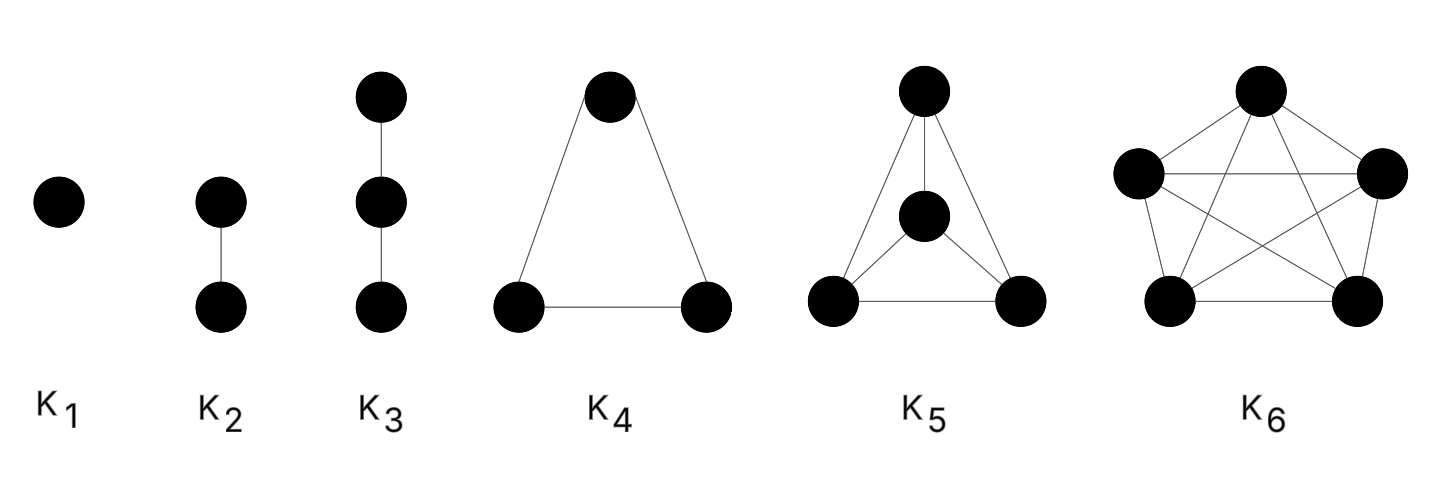
\includegraphics[width=0.8\linewidth,angle=0]{figuras/tiposgrafos/grafo_completo.png}%% Dimensões e localização
	\\
	\centering{Fonte: Criação própria}%% Fonte
\end{figure}

Esse tipo de grafo possui algumas observações:
\begin{itemize}
    \item Ele também é um grafo regular $K_{|V| - 1}$, pois todos os vértices possuem o grau de $(|V|-1)$.
    \item O grafo orientado é completo apenas se todo o par ordenado de vértices distintos é um arco.
    \item O grafo orientado completo com $V$ vértices tem exatamente $|V|\times(|V|-1)$ arcos.
\end{itemize}


\textit{\textbf{Grafo conexo:}} Para todos os pares de vértices $\{v_i, v_j \subset V\}$, existe uma cadeia de arcos e arestas de $v_i$ para $v_j$

\begin{figure} [H]
	\centering
	\caption{Grafo Conexo}%% Legenda
	\label{fig:conexo}%% Rótulo
	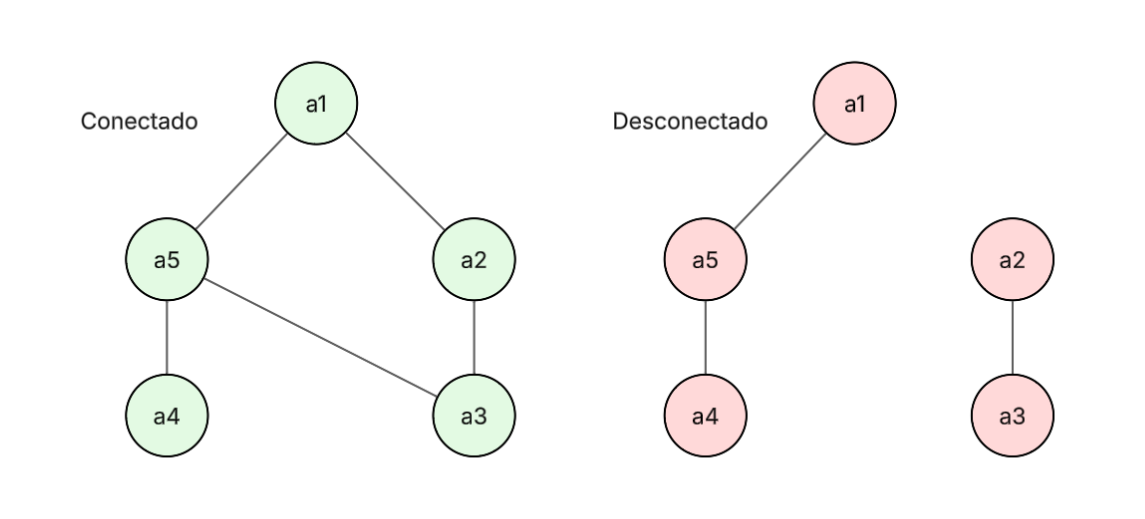
\includegraphics[width=0.8\linewidth,angle=0]{figuras/grafo_conexo.png}%% Dimensões e localização
	\\
	\centering{Fonte: Criação própria}%% Fonte
\end{figure}

Observações:
\begin{itemize}
    \item O grafo $G(V, X)$ é chamado de desconexo, caso exista, pelo menos, um par de vértices que não é ligado por nenhuma cadeia.
    \item O grafo $G(V, X)$ desconexo é formado por, no mínimo dois subgrafos conexos, disjuntamente em relação aos vértices e maximais em relação à inclusão desses.
    \item Um vértice é de corte caso sua remoção, juntamente das arestas conectadas, provoca a redução da conexividade do grafo.
    \item Uma aresta é uma ponte caso sua remoção provoque a redução da conexividade do grafo.
\end{itemize}

\textit{\textbf{Grafo Fortemente Conexo (f-conexo):}} É um grafo direcionado com todos seus pares de vértices ligados por, pelo menos, um caminho de cada sentido. Cada vértice pode se alcançado se parte de qualquer outro vértice e pode alcançar qualquer outro.

\begin{figure} [H]
	\centering
	\caption{Grafo Fortemente Conexo}%% Legenda
	\label{fig:f-conexo}%% Rótulo
	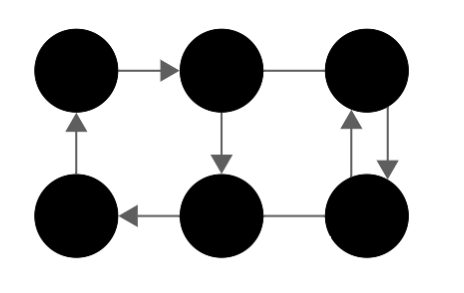
\includegraphics[width=0.4\linewidth,angle=0]{figuras/forte.png}%% Dimensões e localização
	\\
	\centering{Fonte: Criação própria}%% Fonte
\end{figure}


\begin{itemize}
    \item Cada par de vértices participa de um circuito.
    \item O grafo $G(V, E)$ que não é f-conexo é formado por, no mínimo, dois subgrafos fortemente conexos, disjutnos em relação aos vértices e maximais em relação à inclusão.
\end{itemize}

\textbf{Grafo Planar}:
Um grafo é dito planar quando pode ser desenhado em um plano de forma que nenhuma de suas arestas se intercepte com outra.

\begin{figure} [H]
	\centering
	\caption{Grafo Planar}%% Legenda
	\label{fig:planar}%% Rótulo
	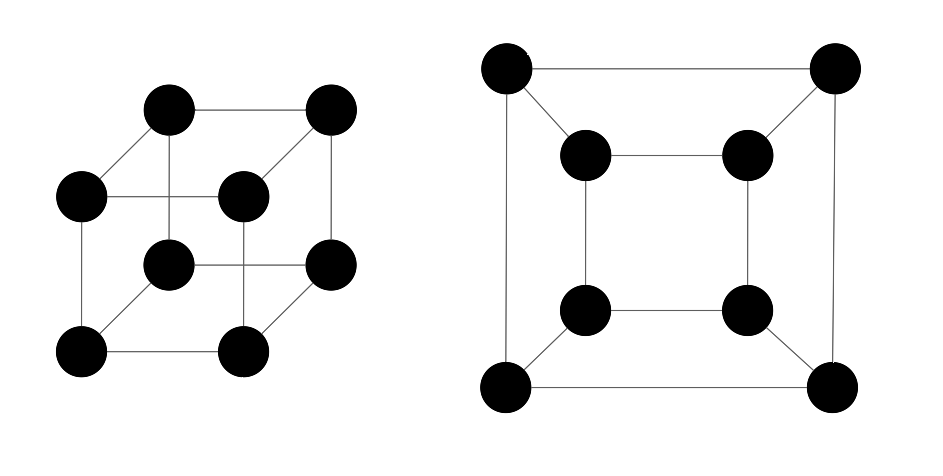
\includegraphics[width=0.4\linewidth,angle=0]{figuras/grafo_planar.png}%% Dimensões e localização
	\\
	\centering{Fonte: Criação própria}%% Fonte
\end{figure}

\textit{Observações:}
\begin{enumerate}
    \item Para $n > 4$, o grafo completo $K_n$ não pode ser representado de forma planar.
    \item As ligações de uma placa de circuito impresso devem obedecer a representações planas, evitando cruzamentos.
    \item O grafo permanece o mesmo; o que varia é apenas sua representação gráfica.
\end{enumerate}

\textbf{Grafo Euleriano}:
Um grafo é euleriano quando admite um ciclo que percorre todas as arestas exatamente uma vez.
Exemplo: $C_{11} = \{u_1, u_2, u_3, u_4, u_5, u_3, u_1, u_6, u_2, u_7, u_3, u_6, u_7, u_1\}$.

\begin{figure} [H]
	\centering
	\caption{Grafo Euleriano}%% Legenda
	\label{fig:euler}%% Rótulo
	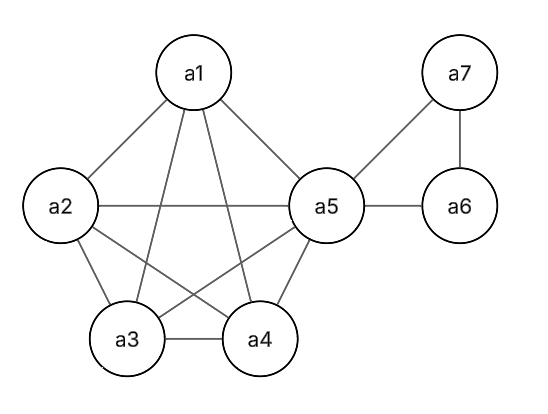
\includegraphics[width=0.4\linewidth,angle=0]{figuras/grafo_euleriano.png}%% Dimensões e localização
	\\
	\centering{Fonte: Criação própria}%% Fonte
\end{figure}

\textbf{Grafo Hamiltoniano}:
Um grafo é dito hamiltoniano quando possui um ciclo que visita todos os vértices exatamente uma vez.

\begin{figure} [H]
	\centering
	\caption{Grafo Hamiltoniano}%% Legenda
	\label{fig:hamilton}%% Rótulo
	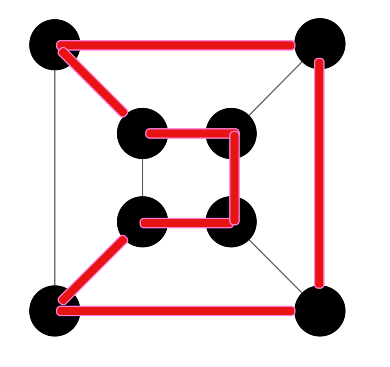
\includegraphics[width=0.2\linewidth,angle=0]{figuras/grafo_hamiltoniano.png}%% Dimensões e localização
	\\
	\centering{Fonte: Criação própria}%% Fonte
\end{figure}

\textbf{Grafo Bipartido}:
Um grafo bipartido é aquele em que o conjunto de vértices pode ser dividido em duas partes disjuntas, $V_A$ e $V_B$, de modo que não existam arestas conectando dois vértices do mesmo conjunto. Toda aresta liga um vértice de $V_A$ a outro de $V_B$.

\begin{figure} [H]
	\centering
	\caption{Grafo Bipartido}%% Legenda
	\label{fig:bipartido}%% Rótulo
	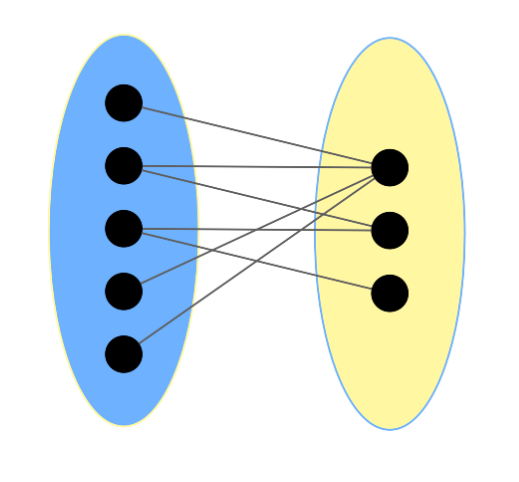
\includegraphics[width=0.3\linewidth,angle=0]{figuras/grafo_bipartido.png}%% Dimensões e localização
	\\
	\centering{Fonte: Criação própria}%% Fonte
\end{figure}

\textbf{Grafo Bipartido Completo}:
É um grafo bipartido no qual cada vértice de $V_A$ está conectado a todos os vértices de $V_B$.

\begin{figure} [H]
	\centering
	\caption{Grafo Bipartido Completo}%% Legenda
	\label{fig:bipartido_completo}%% Rótulo
	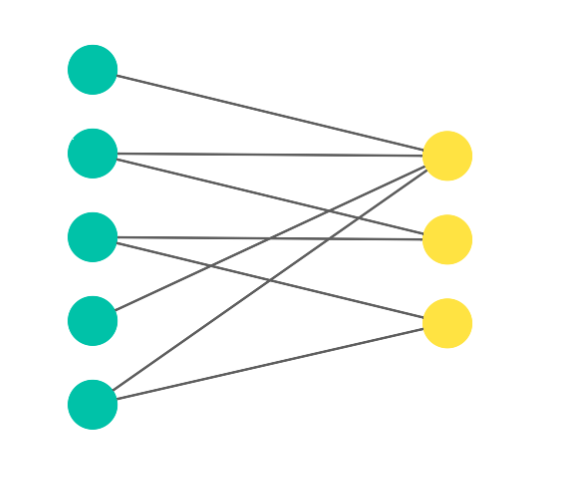
\includegraphics[width=0.4\linewidth,angle=0]{figuras/grafo_bipartido_completo.png}%% Dimensões e localização
	\\
	\centering{Fonte: Criação própria}%% Fonte
\end{figure}

\textbf{Grafo $k$-partido (ou $k$-colorível)}:
Um grafo é $k$-partido quando seus vértices podem ser separados em $k$ subconjuntos disjuntos, sem arestas internas a cada subconjunto.
\textit{Nota:} um grafo $2$-partido é equivalente a um grafo bipartido.

\begin{figure} [H]
	\centering
	\caption{Grafo k-partido}%% Legenda
	\label{fig:kpartido}%% Rótulo
	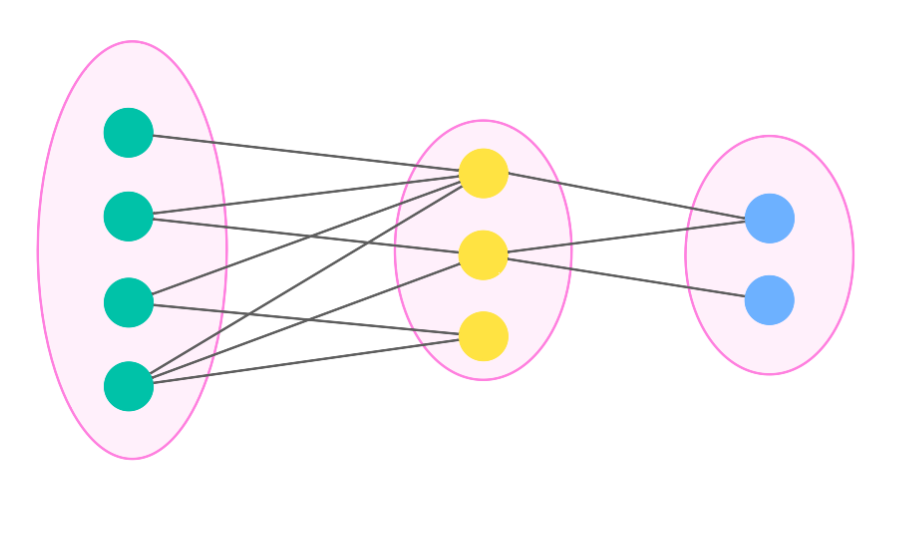
\includegraphics[width=0.4\linewidth,angle=0]{figuras/grafo_k-partido.png}%% Dimensões e localização
	\\
	\centering{Fonte: Criação própria}%% Fonte
\end{figure}

\textbf{Grafo Rotulado}:
Cada vértice (ou aresta) possui associado um identificador ou rótulo.

\textbf{Grafo Ponderado (ou Valorado)}:
É um grafo no qual cada aresta possui um valor (peso) associado. Formalmente, seja $G = (V, X)$, em que $V$ é o conjunto de vértices e $X$ o conjunto de arestas; existe então uma função $P: X \to C_v$, onde $C_v$ representa o conjunto de pesos atribuídos às arestas.

\begin{figure} [H]
	\centering
	\caption{Grafo Ponderado}%% Legenda
	\label{fig:ponderado}%% Rótulo
	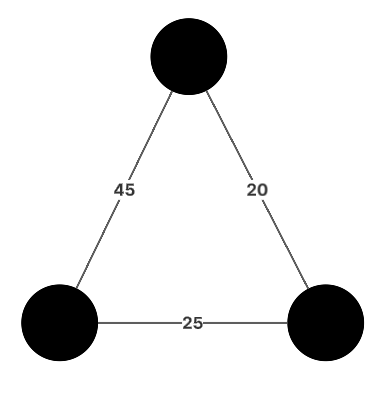
\includegraphics[width=0.2\linewidth,angle=0]{figuras/grafo_ponderado.png}%% Dimensões e localização
	\\
	\centering{Fonte: Criação própria}%% Fonte
\end{figure}

\textit{Observações:}
\begin{enumerate}
    \item Esse tipo de grafo é amplamente utilizado em problemas que envolvem informações quantitativas.
    \item Caso não haja pesos nas arestas, diz-se que o grafo é não ponderado, sendo de interesse apenas a estrutura das conexões.
    \item Exemplo: em um grafo de rotas aéreas, a distância entre dois aeroportos pode ser usada como peso da aresta que os conecta.
\end{enumerate}

\textbf{Grafos Complementares}:
Dado um grafo não orientado $G(V,A)$, o grafo complementar $G^c(V,A')$ é definido pelo mesmo conjunto de vértices $V$, mas em $G^c$ existem arestas justamente onde elas não estão em $G$. Assim:
\[
(v_i, v_j) \in A \implies (v_i, v_j) \notin A' \quad \text{e} \quad (v_i, v_j) \notin A \implies (v_i, v_j) \in A'.
\]

\begin{figure} [H]
	\centering
	\caption{Grafo Complementar}%% Legenda
	\label{fig:complementar}%% Rótulo
	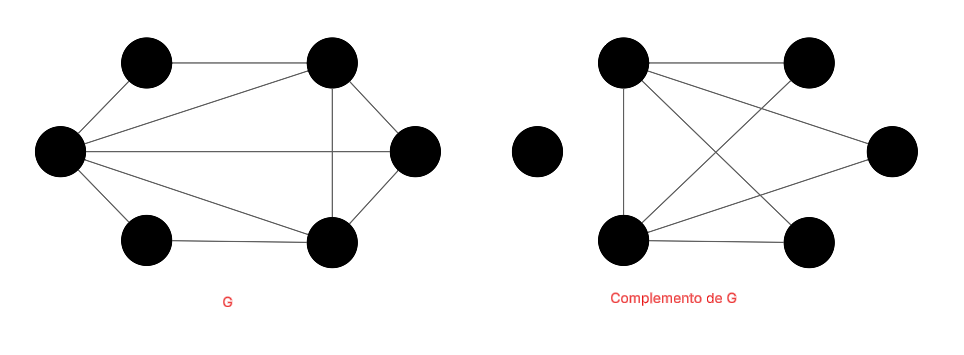
\includegraphics[width=0.4\linewidth,angle=0]{figuras/grafo_complemetnar.png}%% Dimensões e localização
	\\
	\centering{Fonte: Criação própria}%% Fonte
\end{figure}
%IAN

\textbf{Subgrafo gerador ou grafo parcial}:  
Grafo que contém o mesmo conjunto de vértices, porém, com pelo menos uma aresta removida.

\begin{figure}[H]
    \centering
    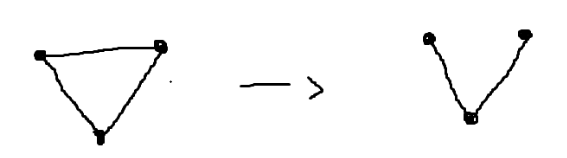
\includegraphics[width=0.6\textwidth]{figuras/Subgrafogerador.png}
    \caption{Exemplo de grafo parcial}
\end{figure}

\medskip

\textbf{Subgrafo induzido}:  
Subgrafo induzido é um subgrafo feito a partir de um conjunto de vértices do grafo original, não podendo ser descartada nenhuma aresta entre o conjunto.

\begin{figure}[H]
    \centering
    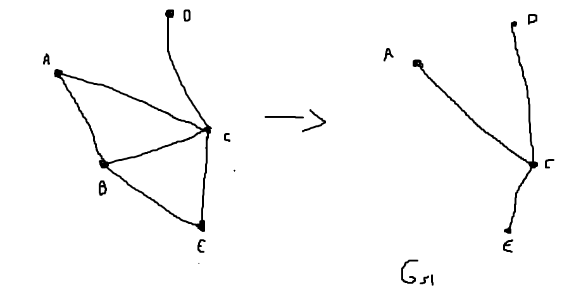
\includegraphics[width=0.6\textwidth]{figuras/Subgrafoinduzido.png}
    \caption{Exemplo de subgrafo induzido}
\end{figure}

\medskip

\textbf{Clique}:  
É um subgrafo completo.

\medskip

\textbf{Árvore}:  
É um grafo não direcionado que tem ordem (quantidade de vértices) maior ou igual a 2.  

É importante ressaltar algumas propriedades para definir se um grafo é uma árvore:
\begin{enumerate}
    \item $G$ é conexo e sem ciclos;
    \item $G$ é sem ciclos e tem $|V|-1$ arestas;
    \item $G$ é conexo e tem $|V|-1$ arestas;
    \item $G$ é sem ciclos e a adição de uma aresta entre dois vértices não adjacentes cria um ciclo e somente um;
    \item $G$ é conexo, mas deixa de sê-lo se uma aresta é suprimida (todas as arestas são pontes);
    \item Todo par de vértices de $G$ é unido por uma e somente uma cadeia simples.
\end{enumerate}

\begin{figure}[H]
    \centering
    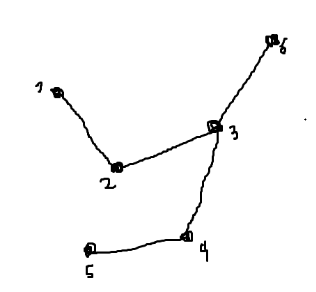
\includegraphics[width=0.6\textwidth]{figuras/Arvore.png}
    \caption{Exemplo de árvore}
\end{figure}

\medskip

\textbf{Árvore geradora de um grafo conexo}:  
É um subgrafo conexo e acíclico que contém todo o conjunto de vértices e um subconjunto de arestas do grafo original.  

Obs: Todo grafo conexo tem pelo menos uma árvore geradora.

\begin{figure}[H]
    \centering
    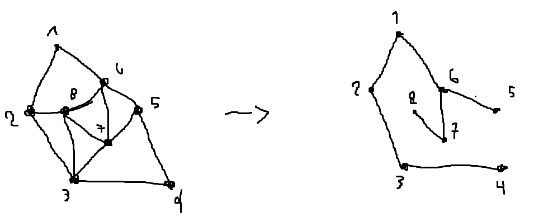
\includegraphics[width=0.6\textwidth]{figuras/Arvoregeradora.png}
    \caption{Exemplo de árvore geradora}
\end{figure}

\medskip

\textbf{Floresta}:  
Um grafo acíclico que pode ser conectado ou não, cujas partes são árvores, sendo uma união de árvores.

\begin{figure}[H]
    \centering
    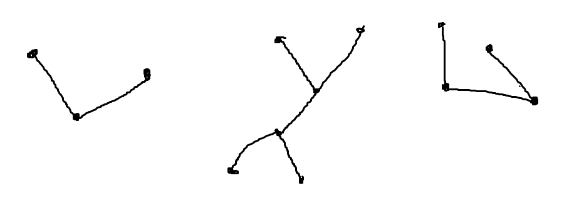
\includegraphics[width=0.6\textwidth]{figuras/Floresta.png}
    \caption{Exemplo de floresta}
\end{figure}

\textbf{Floresta geradora de um grafo}:  
Uma floresta que tem todos os vértices de um grafo.

\medskip

\textbf{Grafos Isomórficos}:  
Um grafo é isomorfo a outro se ele mantém a mesma correspondência de incidências ao outro grafo.  

\begin{figure}[H]
    \centering
    \includegraphics[width=0.6\textwidth]{figuras/Grafoisomorfico.png}
    \caption{Exemplo de grafo isomorfo}
\end{figure}

Obs:
\begin{enumerate}
    \item Se um grafo $G_2$ é isomorfo a $G_1$, então $G_1$ é isomorfo a $G_2$.
    \item Se um grafo $G_2$ é isomorfo a $G_1$ e $G_3$, então $G_3$ é isomorfo a $G_2$ e vice-versa.
    \item Um grafo é isomorfo a si próprio.
    \item Um grafo $G_2$, se isomorfo a $G_1$, carrega as mesmas propriedades de $G_1$.
\end{enumerate}

\medskip

\textbf{Conjunto independente de vértices}:  
É um conjunto de pelo menos dois vértices de um grafo que não são adjacentes entre si.

\begin{figure}[H]
    \centering
    \includegraphics[width=0.6\textwidth]{figuras/Conjuntoidepen.png}
    \caption{Exemplo de conjunto independente de vértices}
\end{figure}

Exemplos de conjuntos independentes de vértices do grafo da imagem:
\[
S_1 = \{1,3\}, \quad
S_2 = \{2,4,6\}, \quad
S_3 = \{5,1,3\}
\]

\medskip

\textbf{Grafo misto}:  
Quando um grafo pode possuir simultaneamente arestas e arcos.

\medskip

\textbf{Hipergrafo}:  
Grafo não orientado onde cada aresta conecta um número arbitrário de vértices.

\begin{figure}[H]
    \centering
    \includegraphics[width=0.6\textwidth]{figuras/Hipergrafo.png}
    \caption{Exemplo de hipergrafo}
\end{figure}

Exemplo:
\[
\text{Arestas} = \{1,2,4\}, \{1,3,4\}, \{1,3\}
\]

\chapter{Operações}\label{cap:operacoes}

A estrutura de dados grafos permitem algumas operações matemáticas nos seus conjuntos de vértices e arestas de modo a facilitar a execução de alguns algoritmos. As principais operações são: união, intersecção, soma, decomposição, remoção, fusão e contração. Cada uma delas são exemplificadas, respectivamente, nas Seções \ref{sec:uniao}, \ref{sec:interseccao}, \ref{sec:soma}, \ref{sec:decomposicao}, \ref{sec:remocao}, \ref{sec:fusao} e \ref{sec:contracao}.

\section{União}\label{sec:uniao}
A união de dois grafos, sendo eles $G_1 = (V_1, A_1)$ e $G_2 = (V_2, A_2)$, é dada por:
\[
	G_1 \cup G_2 = (V_1 \cup V_2, A_1 \cup A_2)
\]

Esta é uma operação que apenas une os vértices e arestas dos grafos envolvidos, não adicionando nenhuma outra parte.
Temos como exemplo a adição do $Sub\_Grafo1$ ao grafo $Sub\_Grafo2$.
Onde $Sub\_Grafo1 = (V_1, V_2, V_3, V_6, V_{10}, V_{11}, a_1, a_2, a_4, a_5, a_{10}, a_{11} )$ e $Sub\_Grafo2 = (V_6, V_9, V_{10}, V_{11}, V_{13}, V_{14}, V_{15}, A_{9}, A_{10}, A_{11}, A_{16}, A_{17}, A_{18}, A_{20}, A_{21})$.

% TEMPLATE ADICIONAR IMAGEM EM LATEX
% \begin{figure}[!h]
%     \centering
% 	\label{fig:uniaoGrafos}
% 	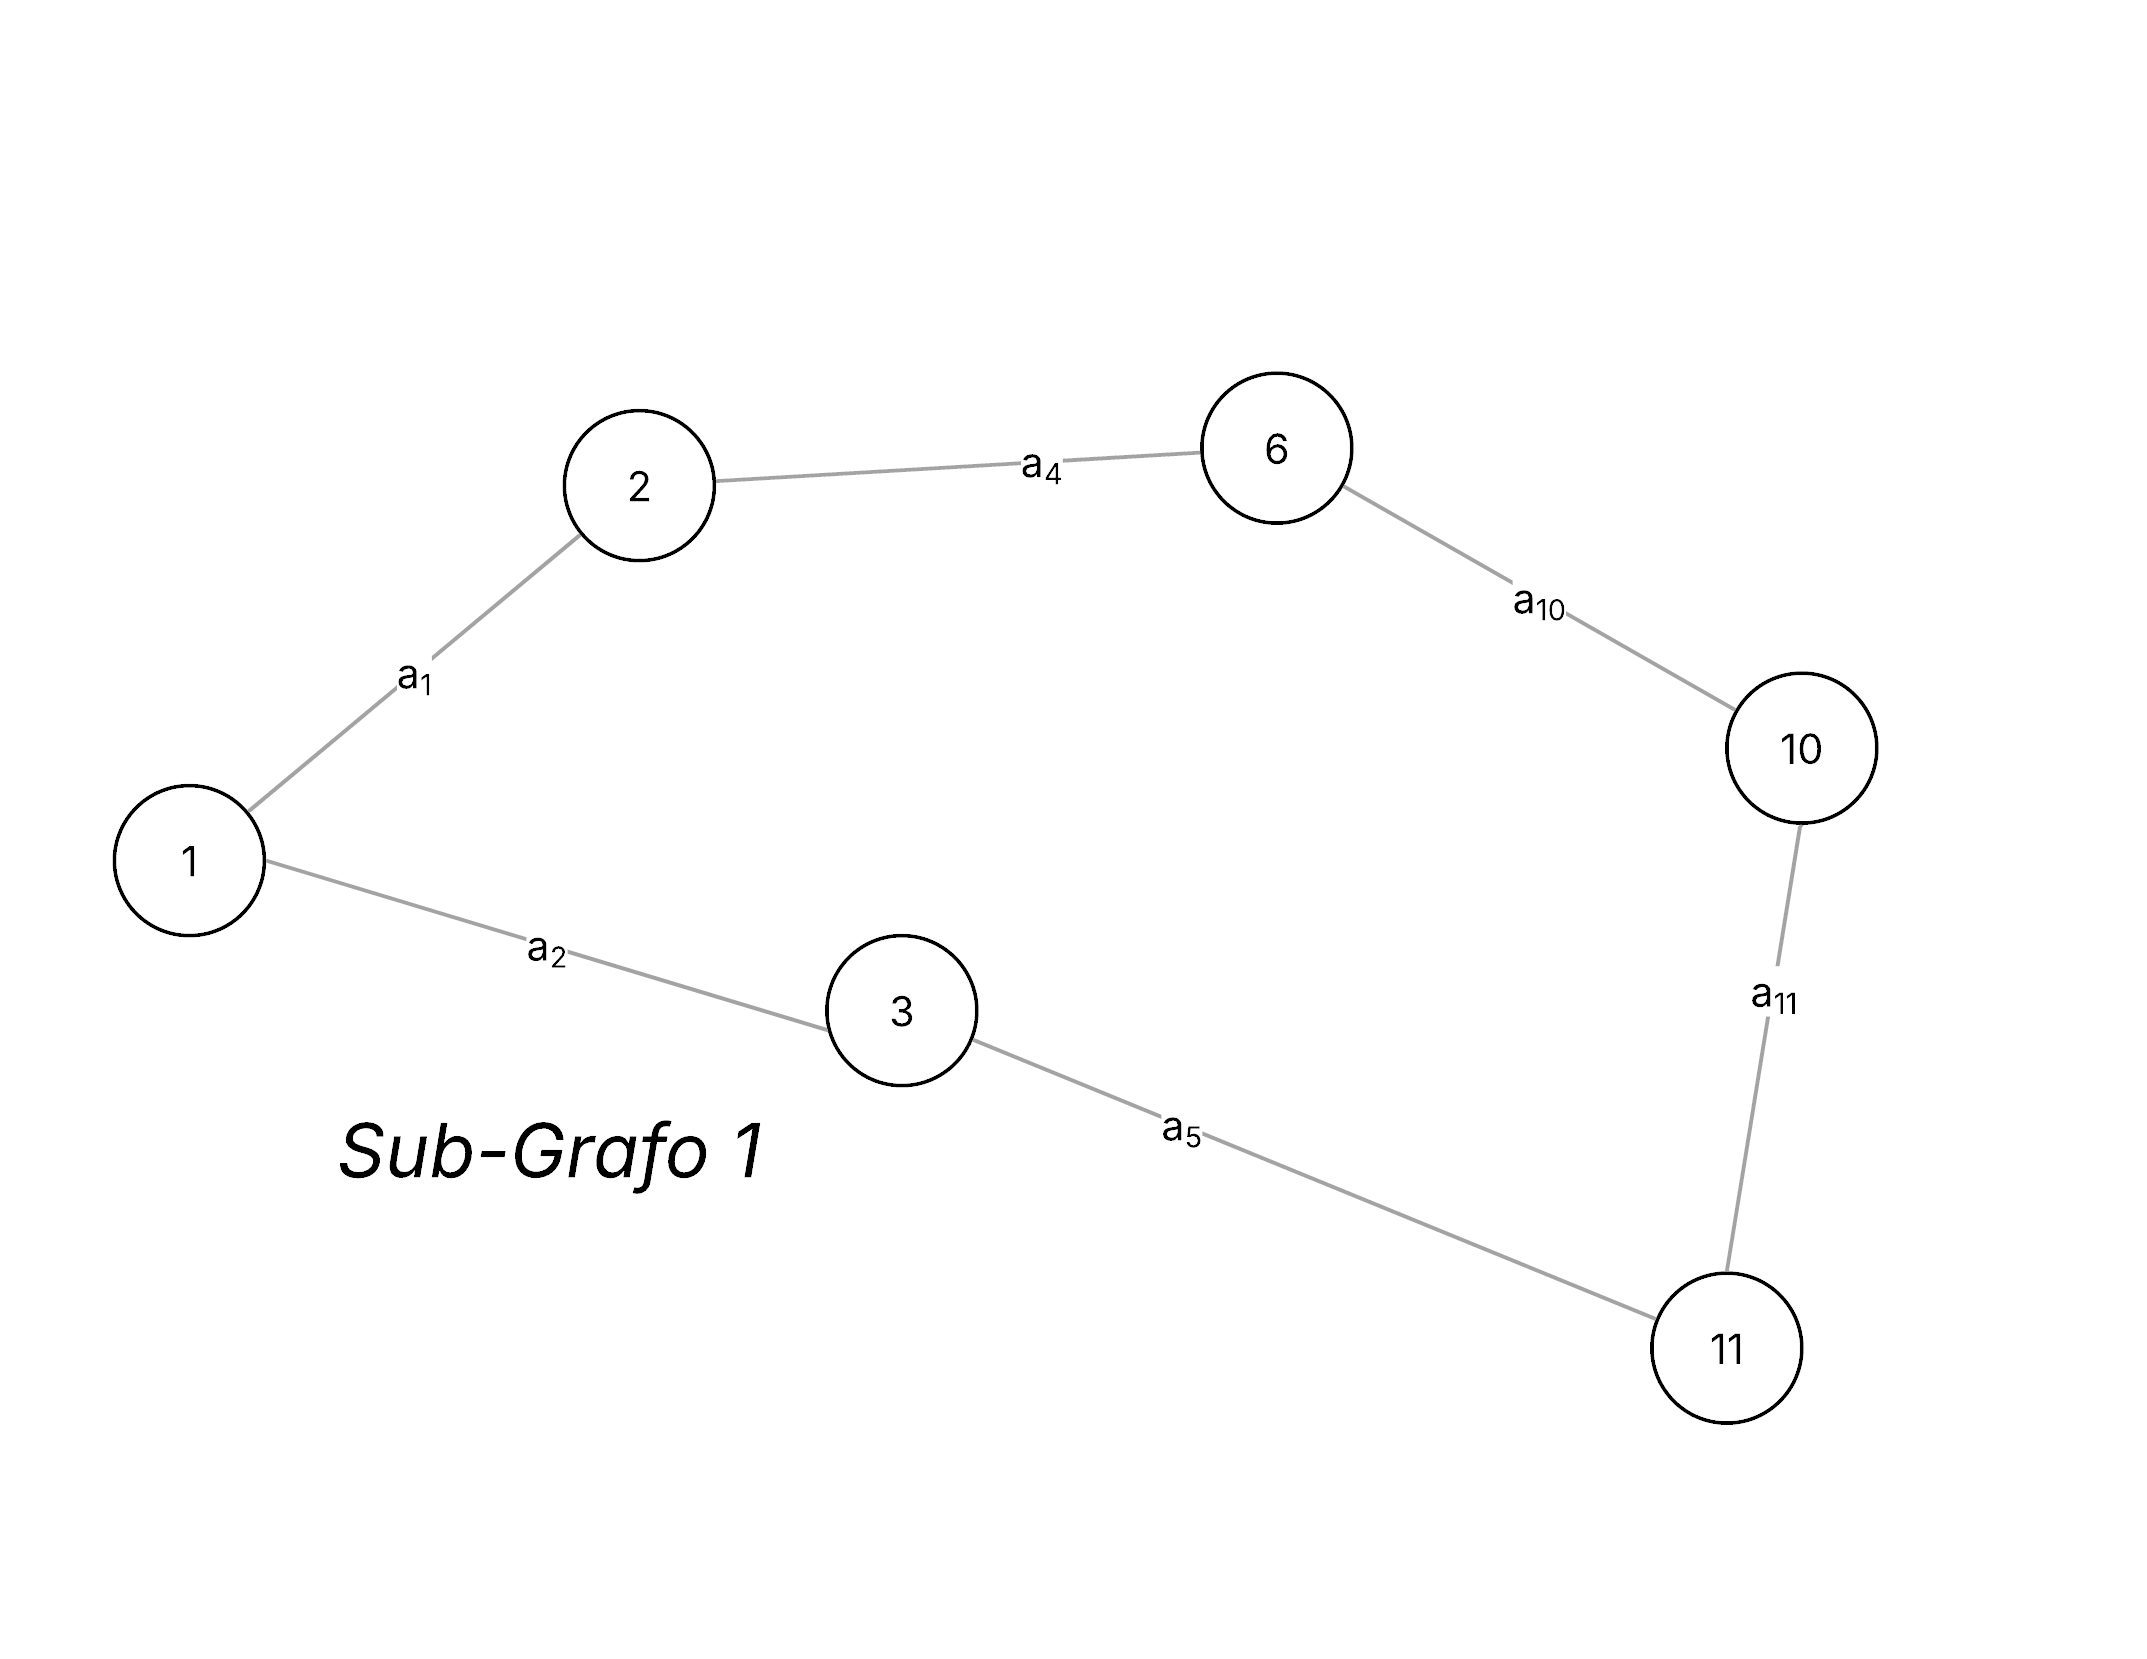
\includegraphics[width=0.7\textwidth]{figuras/subgrafos/subgrafo1.png}
% 	\caption{subgrafo 1}
% \end{figure}
\begin{figure}[!htb]
	\centering % Centraliza o conjunto de subfiguras na página

	\begin{subfigure}[b]{0.48\textwidth}
		\centering
		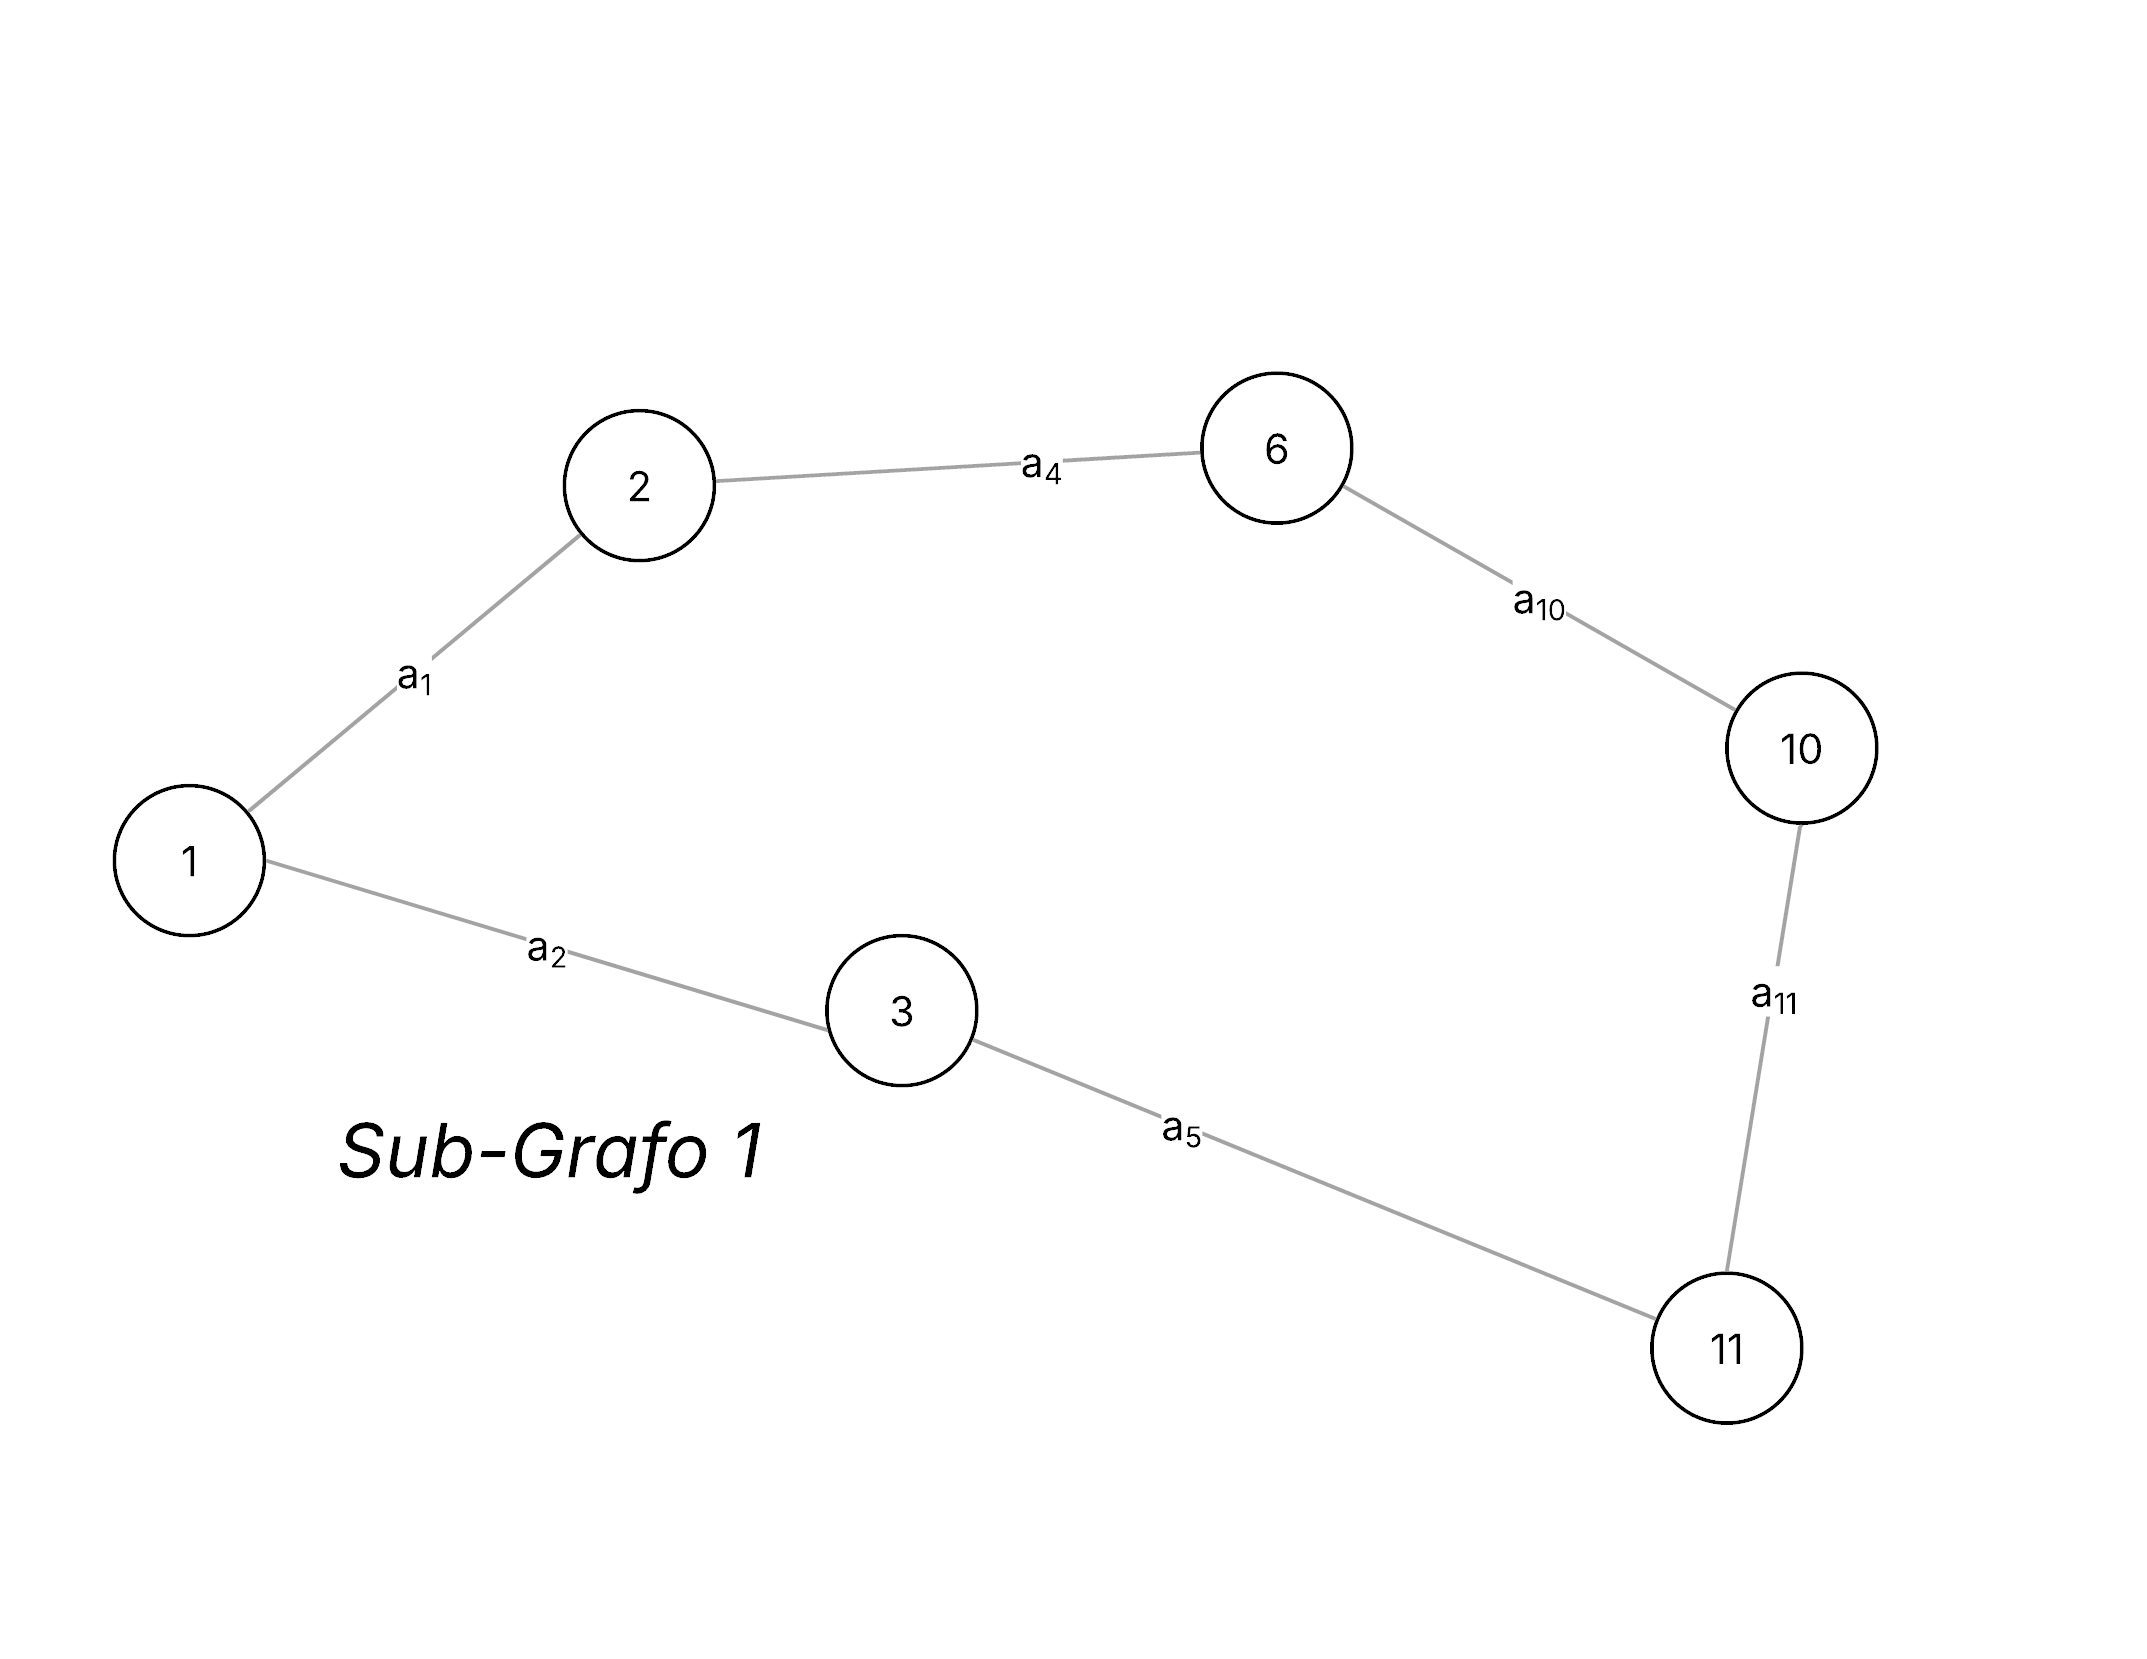
\includegraphics[width=\textwidth]{figuras/subgrafos/subgrafo1.png} % Substitua pelo caminho da sua imagem
		\caption{subgrafo 1}
		\label{fig:imagem1}
	\end{subfigure}
	\hfill % Adiciona um espaço flexível entre as imagens
	\begin{subfigure}[b]{0.48\textwidth}
		\centering
		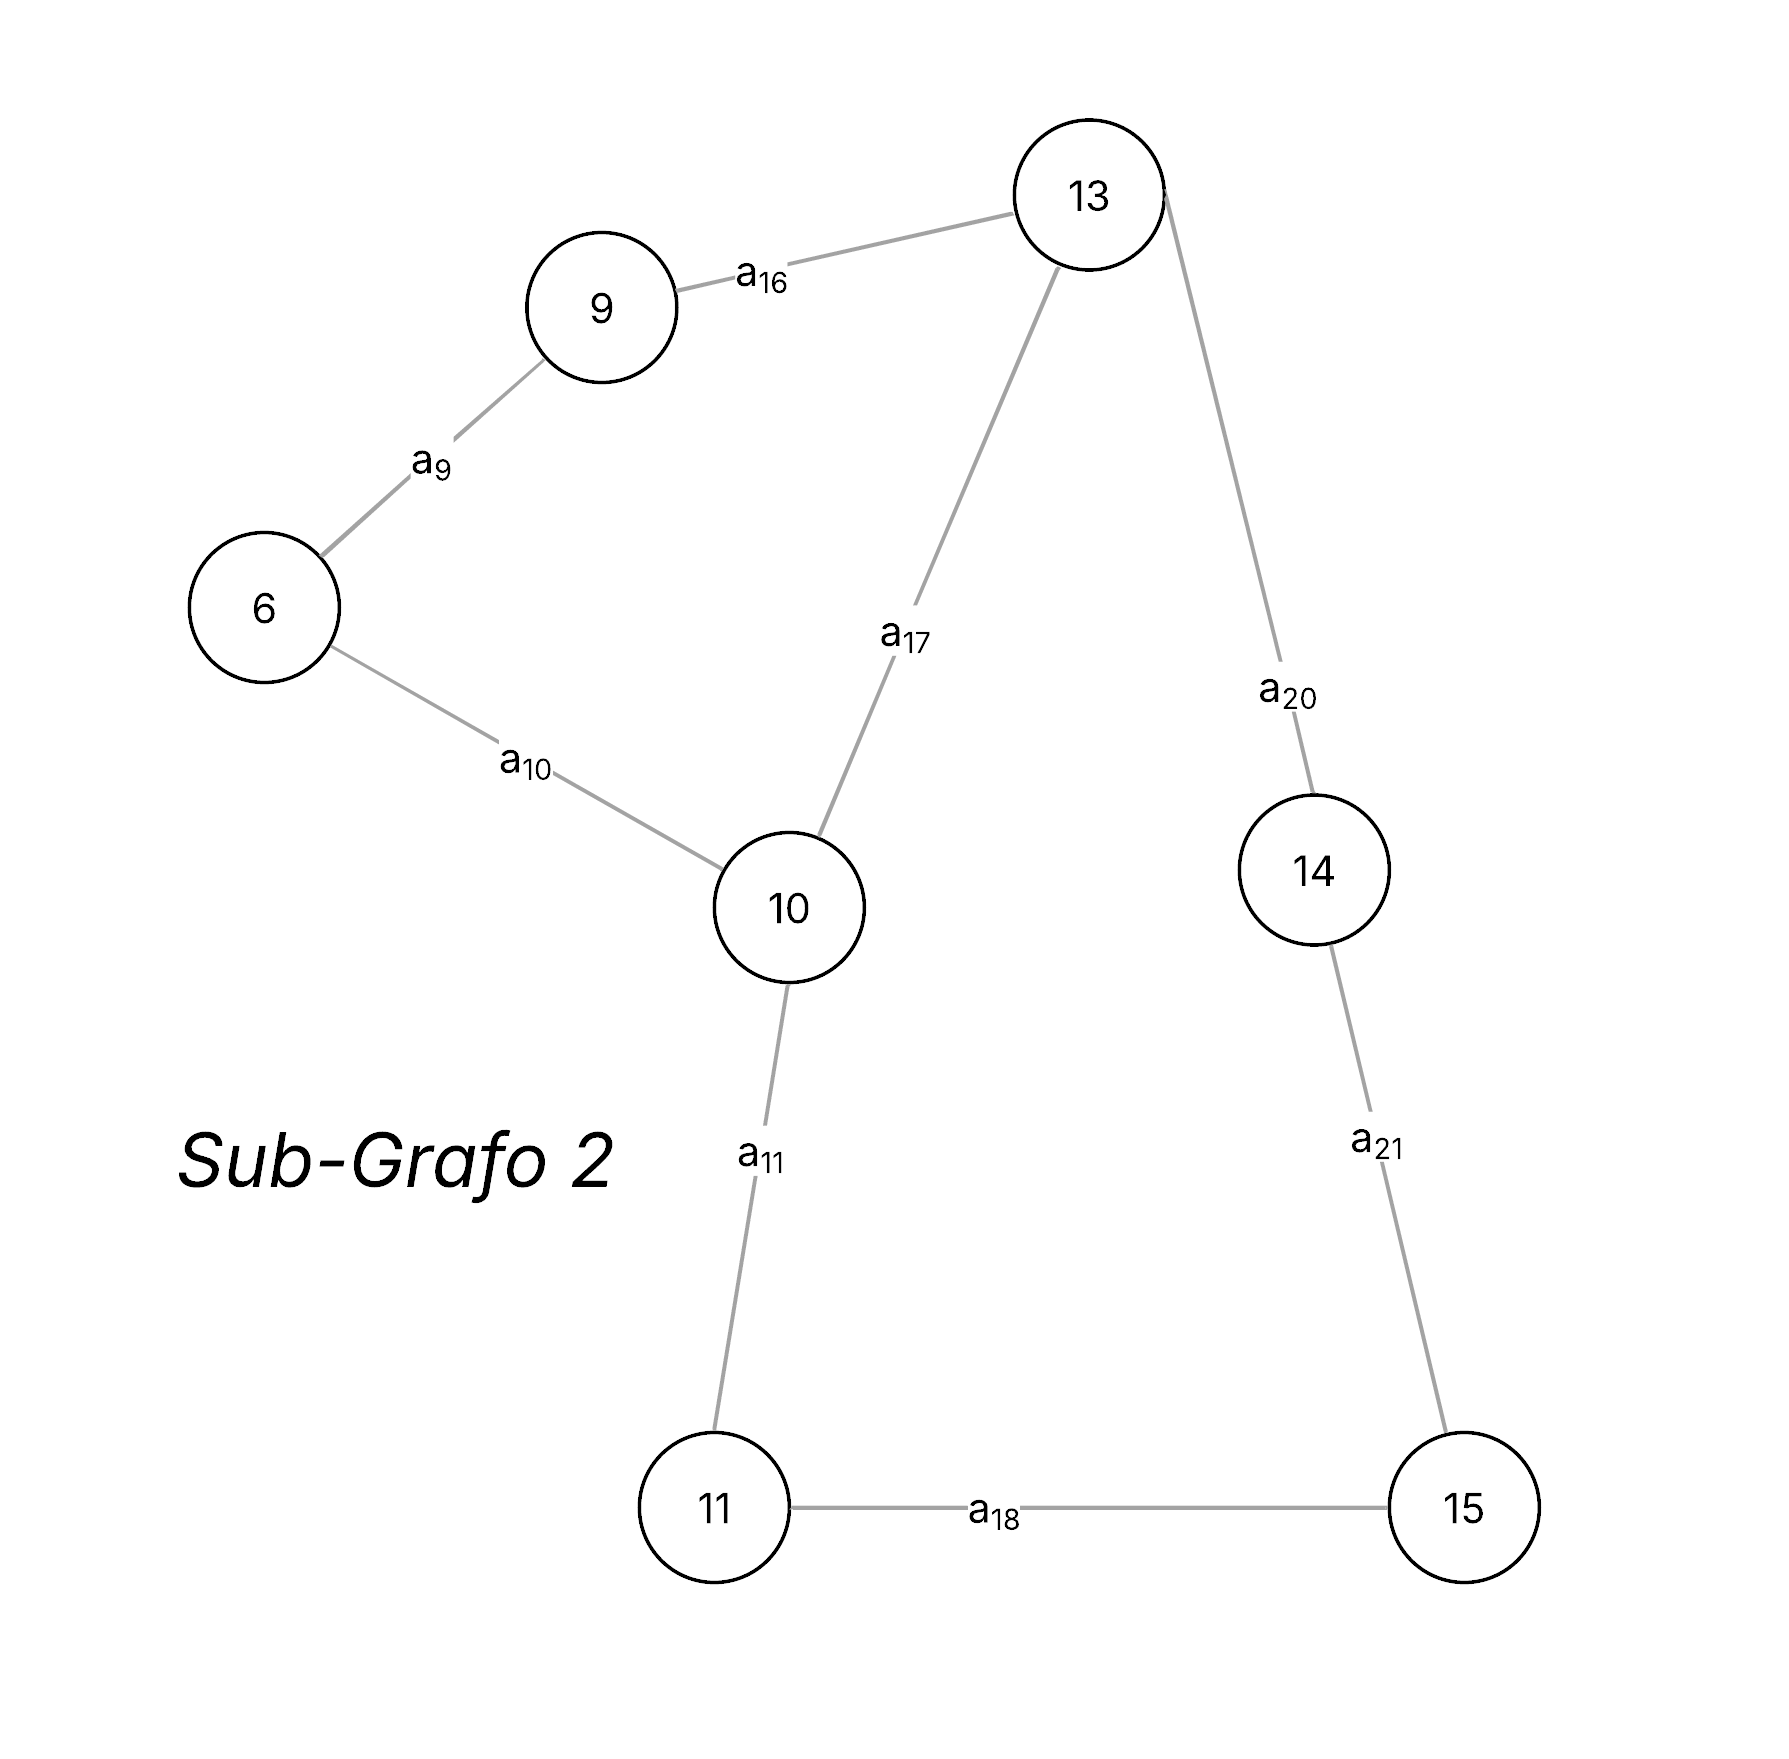
\includegraphics[width=\textwidth]{figuras/subgrafos/subgrafo2.png} % Substitua pelo caminho da sua imagem
		\caption{subgrafo 2}
		\label{fig:imagem2}
	\end{subfigure}

	\caption{subgrafos}
	\label{fig:duasFiguras}
\end{figure}

A aplicação da operação de união resultaria em $Sub\_Grafo1 \cup Sub\_Grafo2$, representando graficamente se dá na figura seguinte:

\begin{figure}
	\centering
	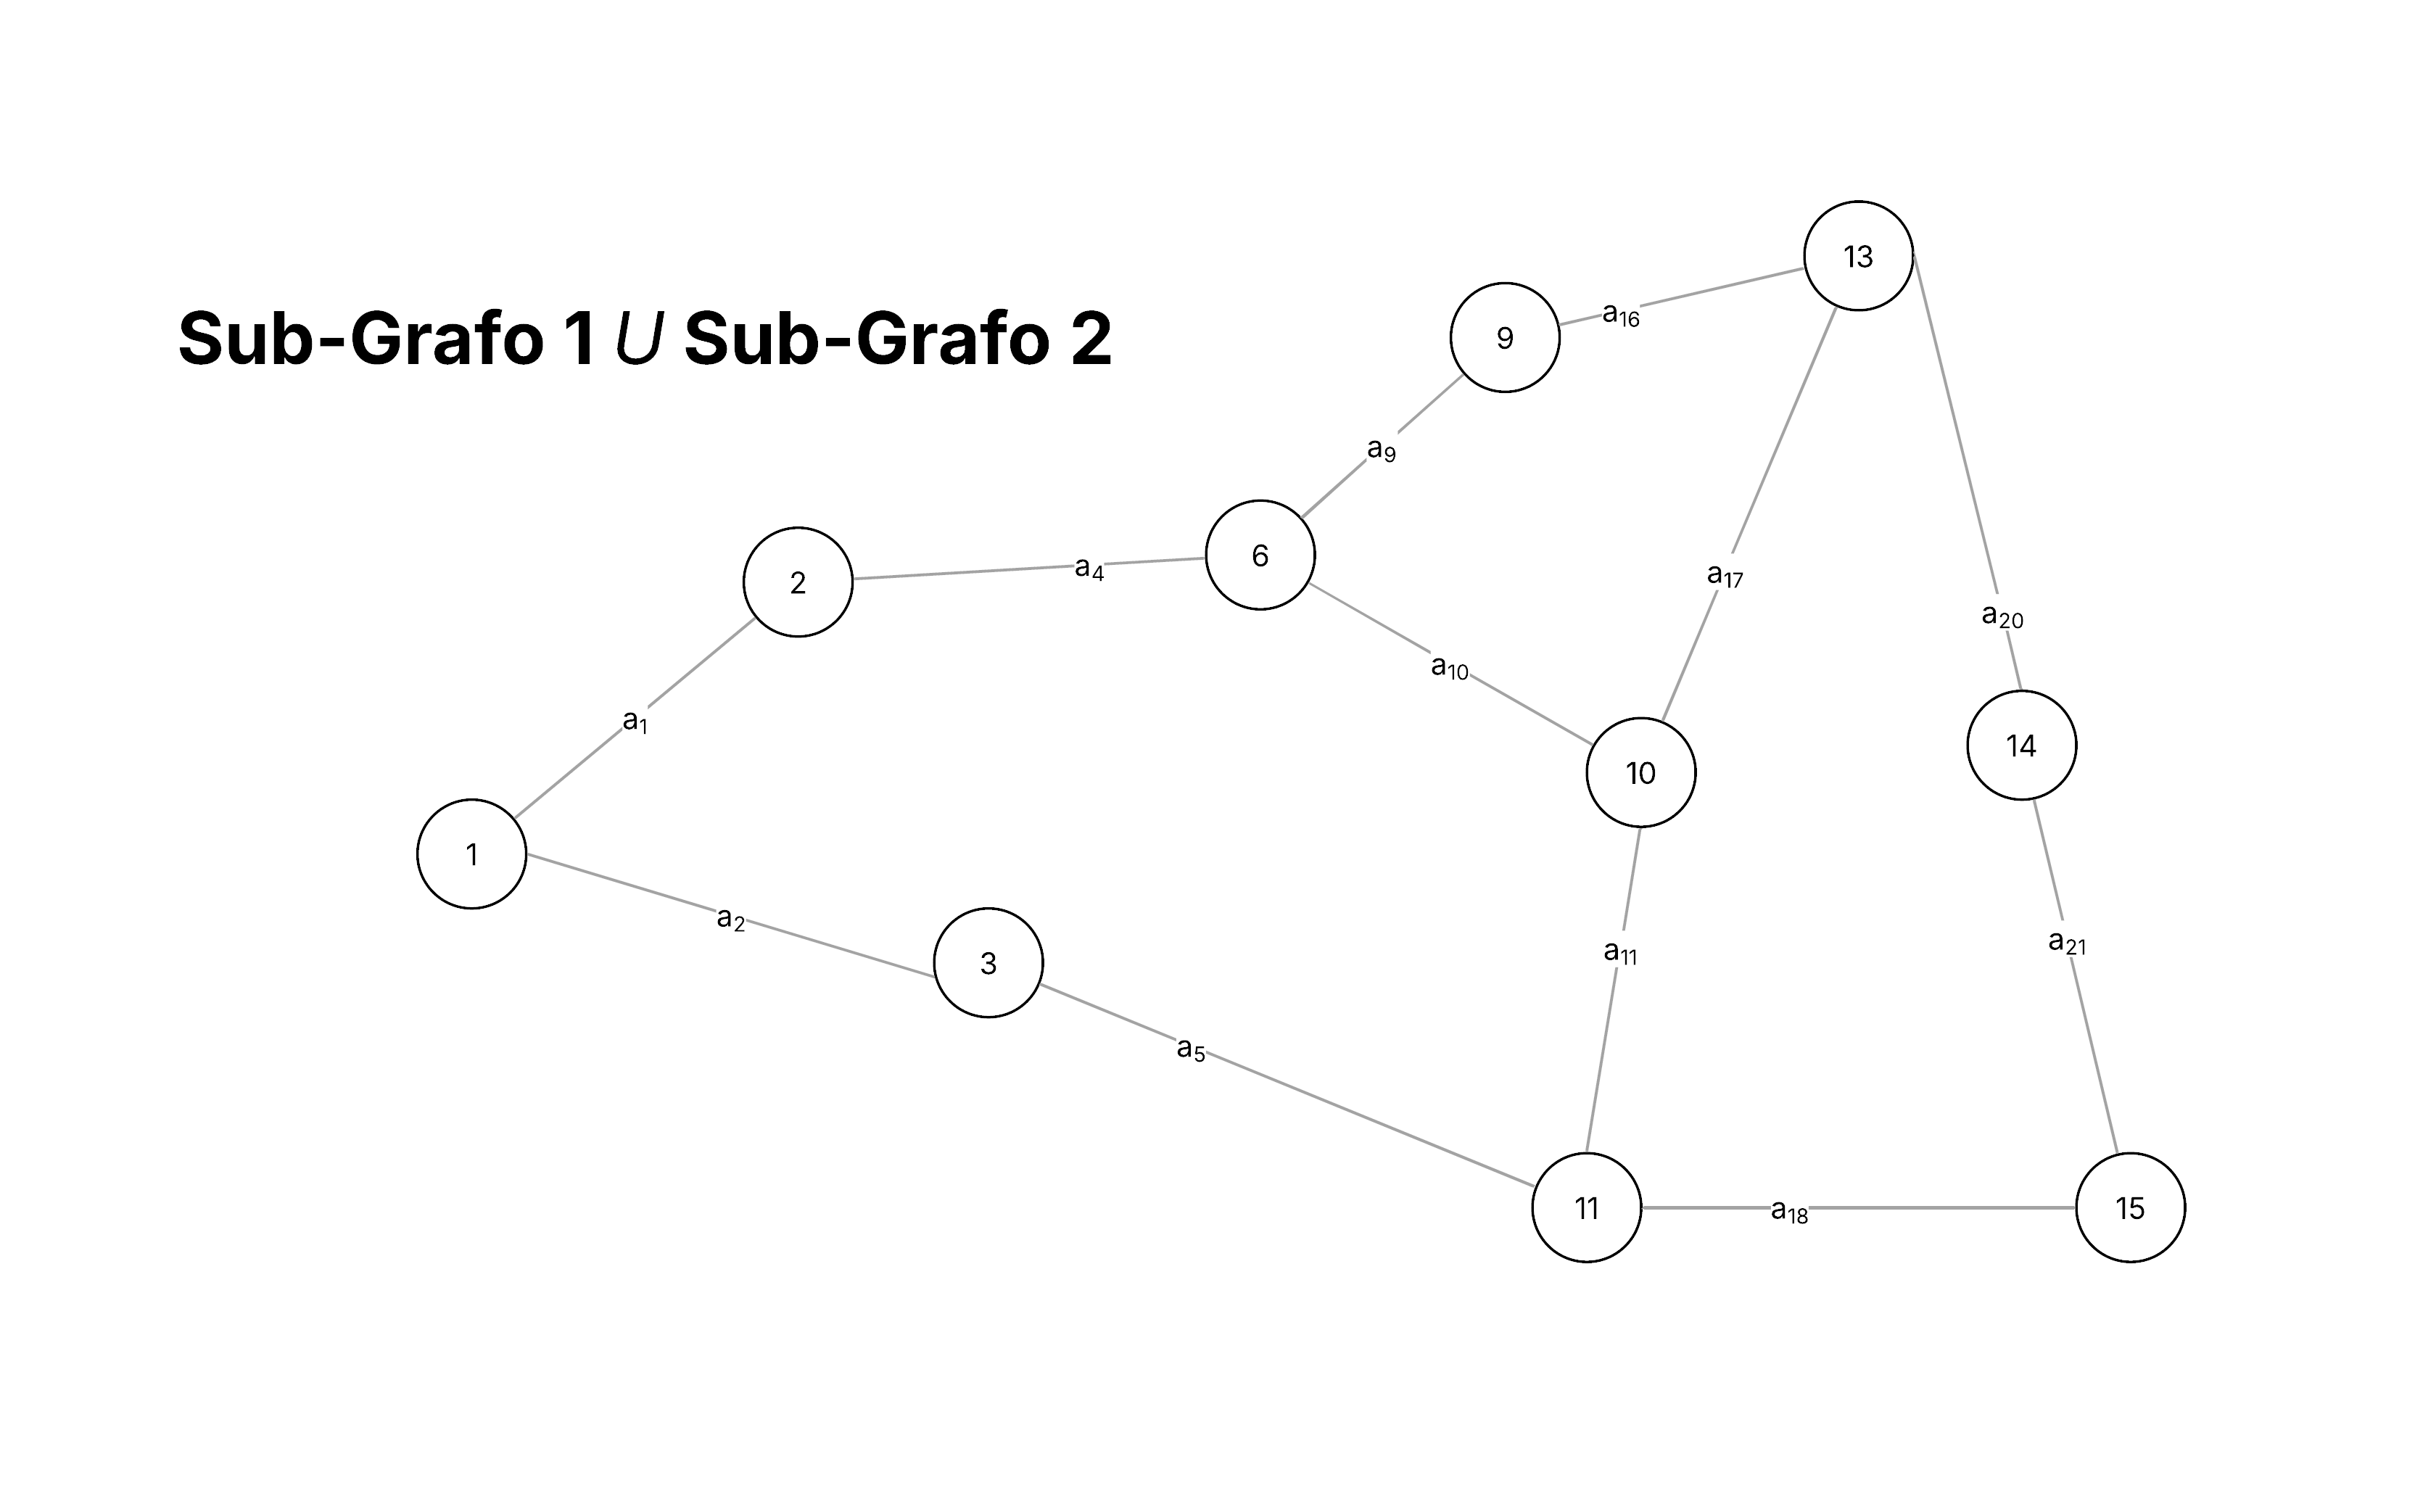
\includegraphics[width=0.8\textwidth]{figuras/subgrafos/subgrafo1usubgrafo2.png}
	\caption{União dos subgrafos}
	\label{fig:uniaoGrafos}
\end{figure}

\section{Intersecção}\label{sec:interseccao}
A intersecção de dois grafos, sendo eles $G_1 = (V_1, A_1)$ e $G_2 = (V_2, A_2)$, gera um terceiro grafo, esse que é apenas o conjunto onde os dois grafos se encontram, ou seja, os vértices e arestas que são comuns aos dois grafos. Quando os grafos intersectam e resultam em nulos ou vazios $V_3 = 0$. A intersecção é dada por:
\[
	G_3 = G_1 \cap G_2 = (V_1 \cap V_2, A_1 \cap A_2)
\]

Sendo $G_3$ a intersecção de $G_1$ e $G_2$, $G_3$ é um subgrafo de ambos os grafos originais.
Aplicando a operação de intersecção nos subgrafos da seção \ref{sec:uniao}, temos:

\begin{figure}[!h]
	\centering
	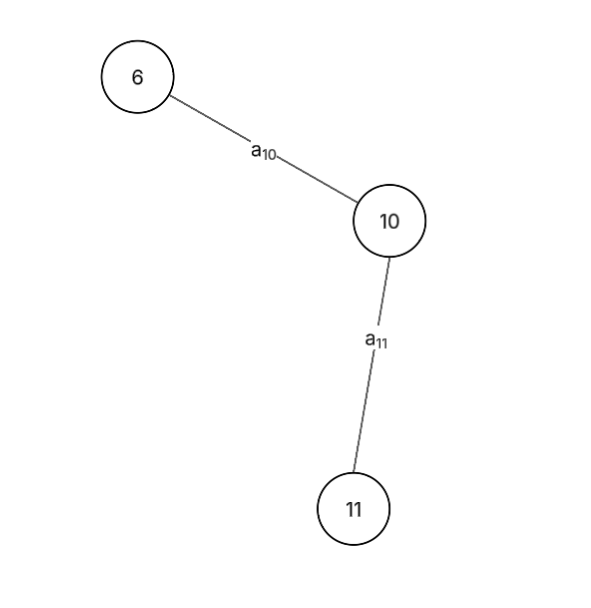
\includegraphics[width=0.4\textwidth]{figuras/subgrafos/subgrafo_inter.png}
	\caption{Intersecção dos subgrafos da figura 4.1}
	\label{fig:intersecaoGrafos}
\end{figure}

\section{Soma}\label{sec:soma}
A soma de dois grafos é dividida entre dois tipos, a soma e soma direta.
A soma junta os vértices e arestas dos dois grafos, criando uma conexão intercomplexa. A soma dos grafos resulta em um novo, como $G_3 = G_1 + G_2$ A fórmula é dada por:
\[
	G_3 = G_1 + G_2 = (V_1 \cup V_2, A_1 \cup A_2 \cup \{ \forall vi \in V_1, \forall vj \in V_2, \exists(vi, vj) \})
\]

\begin{figure}[!h]
	\centering
	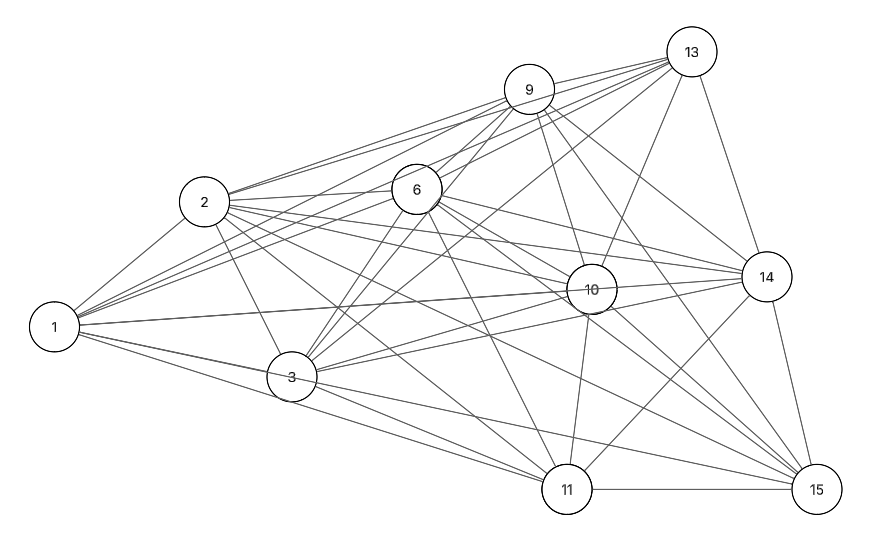
\includegraphics[width=0.9\textwidth]{figuras/soma_NOVO.png}
	\caption{Soma dos subgrafos da figura 4.1}
	\label{fig:somaGrafos}
\end{figure}

Seguindo o exemplo, utilizando as fig \ref{sec:uniao} novamente, podemos observar as novas arestas serem criadas, se diferindo da soma direta, a qual é uma forma de combinar dois grafos baseados em multiplicação estrutural. O conjunto de vértices resultante do produto cartesiano dos conjuntos de vértices dos grafos originais, sendo todos pares ordenados, onde o primeiro elemento pertence a $V_1$ e o segundo a $V_2$.

\[
	V_3 = V_1 \times V_2 = \{(u,v):u\in V_1,\; v\in V_2\}
\]

O conjunto de arestas se baseia na regra da adjacência, uma aresta entre dois vértices $(u, v)$ e $(u_1, v_1)$ em $V_3$ se e somente se eles são adjacentes em $G_1$ e $G_2$, tendo assim um grafo  $G_1 \times G_2$. Traduzindo para a fórmula:

\[ %SOMA DIRETA%
	G_3 = G_1+G_2=\big(V_1\cup V_2,\;E_1\cup E_2\cup \{\{u,v\}:u\in V_1,\; v\in V_2\}\big).
\]

\begin{figure}[!h]
	\centering
	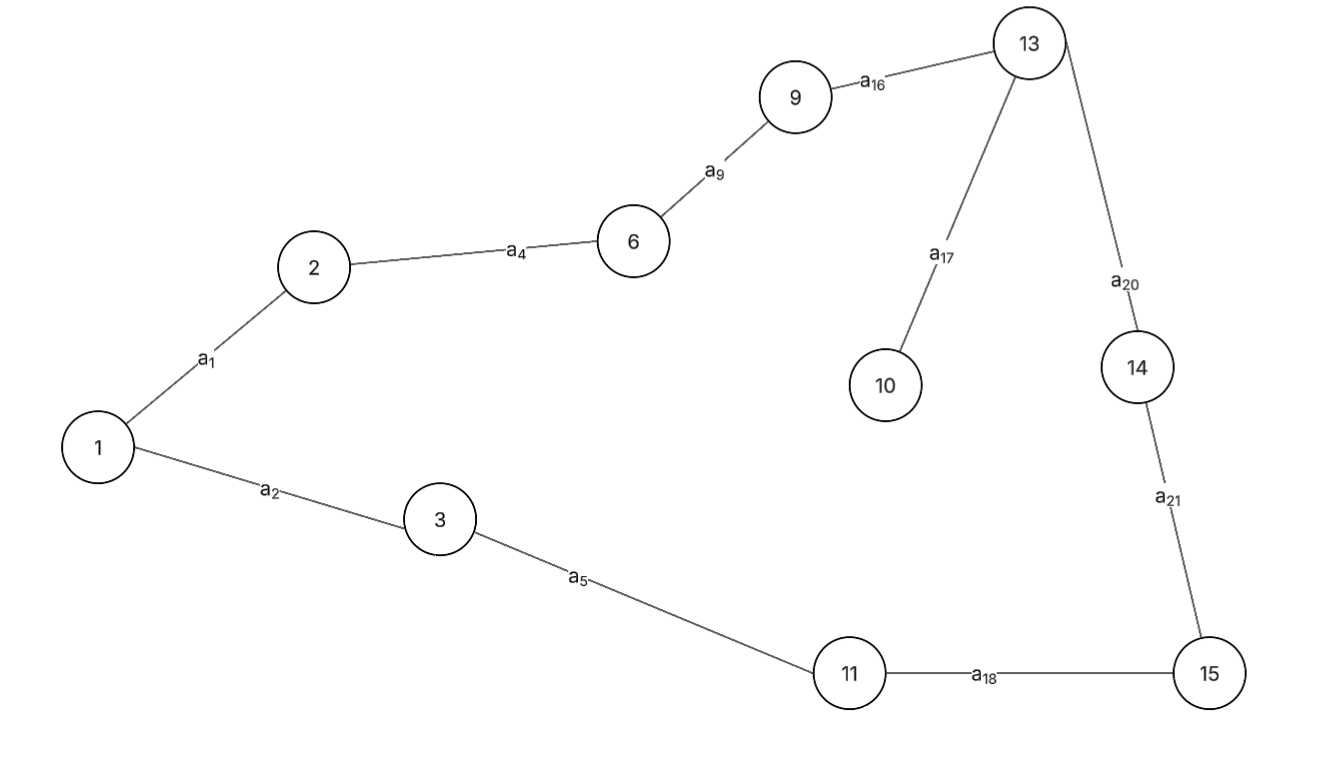
\includegraphics[width=0.6\textwidth]{figuras/subgrafos/subgrafo_soma_direta.png}
	\caption{Soma Direta dos subgrafos da figura 4.1}
	\label{fig:somaDiretaGrafos}
\end{figure}

% Soma direta
% soma
\section{Decomposição}\label{sec:decomposicao}
A decomposição de um grafo $G$ é a partição de seu conjunto de arestas em subgrafos distintos, sendo assim, um grafo é decomposto em dois subgrafos $G_1$ e $G_2$ se a união original é $G_3 = G_1 \cup G_2$ e sua intersecção é um grafo nulo $G_1 \cap G_2 = V_0$, implicando que $G$ pertence exclusivamente a $G_1$ ou $G_2$. Decompondo o subgrafo de fig. \ref{sec:soma} temos os subgrafos originais (a) e (b) de fig. \ref{sec:uniao}.

\begin{figure}[!h]
	\centering
	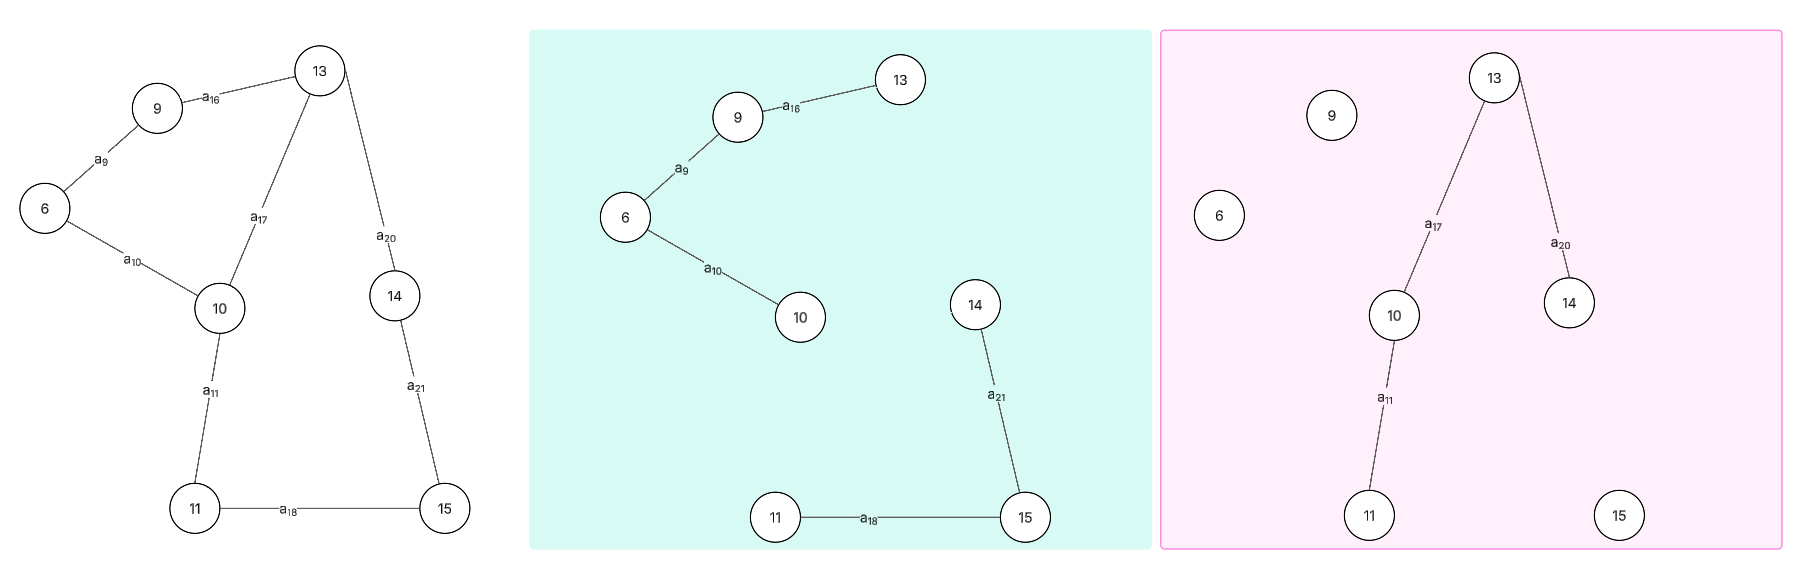
\includegraphics[width=1\textwidth]{figuras/decomposicao.png}
	\caption{Decomposição do subrafo da figura 4.1}
	\label{fig:decomposicao}
\end{figure}

\section{Remoção}\label{sec:remocao}
A remoção de um vértice ou aresta de um grafo $G$ resulta em um subgrafo $G'$, junto com todas as arestas incidentes ao vértice removido. A remoção de uma aresta/arco é representada por $G - a$ e a remoção de um vértice é representada por $G - v$. O impacto da remoção na conectividade de um grafo é uma métrica crucial para a avaliação de robustez do grafo.

A remoção de uma aresta pode aumentar o número de componentes interligados se a aresta for uma ponte, ou seja, se sua remoção desconecta o grafo. Do mesmo jeito, a remoção de um vértice pode ocasionar um efeito similar se o vértice for um ponto de articulação.

Aplicando a remoção do $V_3$ no subgrafo (a) da seção \ref{sec:uniao} e a remoção das arestas $A_{18}$ e $A_{21}$, obtemos o grafo seguinte:

\begin{figure}[!h]
	\centering % Centraliza o conjunto de subfiguras na página

	\begin{subfigure}[b]{0.48\textwidth}
		\centering
		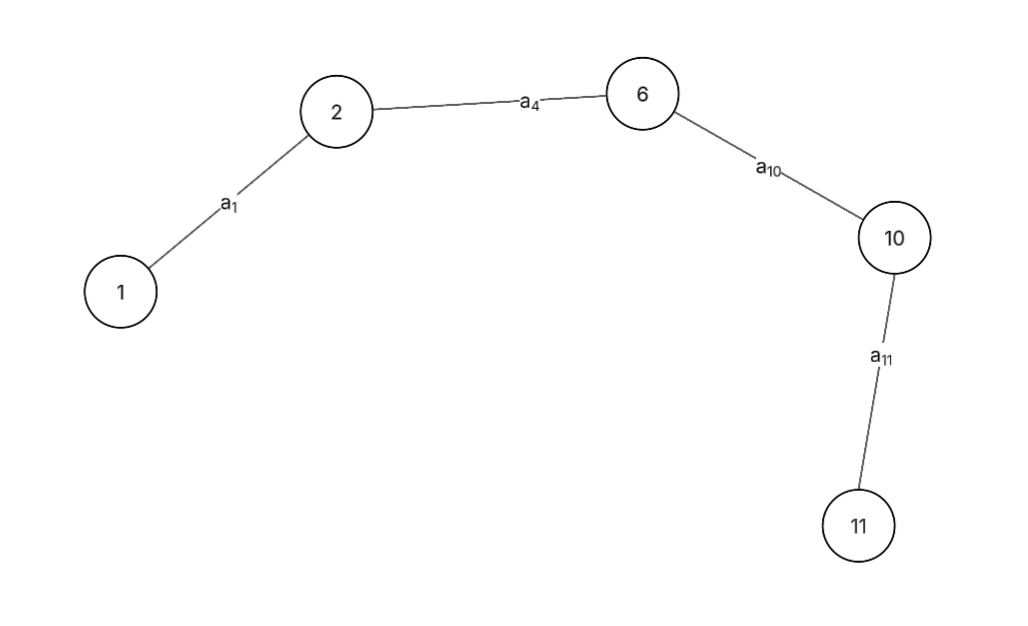
\includegraphics[width=0.8\textwidth]{figuras/subgrafos/subgrafo_remocao_vertice.png} % Substitua pelo caminho da sua imagem
		\caption{Remoção de vértice do subgrafo 4.1. (a)}
		\label{fig:remocaoVertice}
	\end{subfigure}
	\hfill % Adiciona um espaço flexível entre as imagens
	\begin{subfigure}[b]{0.48\textwidth}
		\centering
		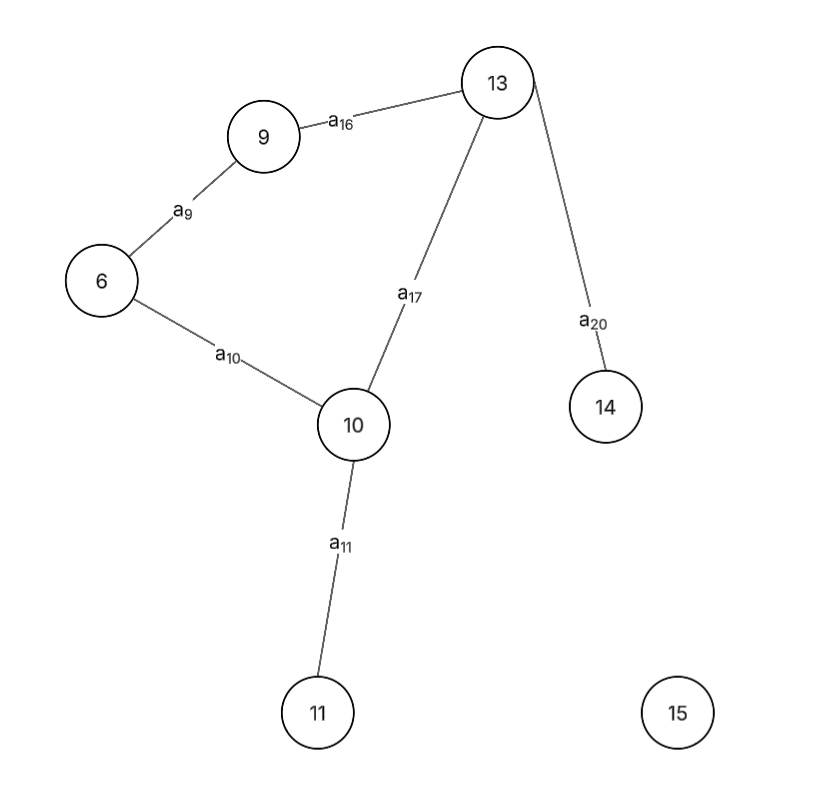
\includegraphics[width=0.8\textwidth]{figuras/subgrafos/subgrafo_remocao_aresta.png} % Substitua pelo caminho da sua imagem
		\caption{Remoção de arestas do subgrafo 2 4.1. (b)}
		\label{fig:remocaoAresta}
	\end{subfigure}

	\caption{Remoções}
	\label{fig:duasRemocoes}
\end{figure}

% Remoção de uma aresta/arco
% remoção de um vértice
\section{Fusão de vértices}\label{sec:fusao}
A fusão de vértices é uma operação que transforma um grafo ao substituir dois ou mais vértices por um único vértice, mantendo as arestas que conectam os vértices originais ao novo vértice. Uma característica distintiva da fusão é que ela reduz o número de vértices do grafo em uma unidade, mas o número total de arestas permanece inalterado.Essa operação é útil em várias aplicações, como simplificação de grafos e redução de complexidade.

\begin{figure}[!h]
	\centering
	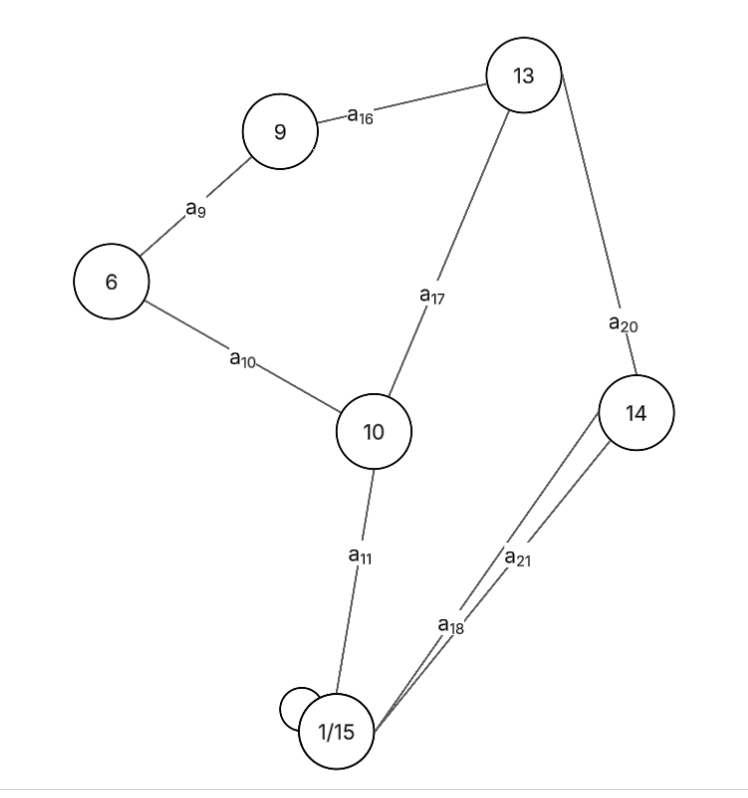
\includegraphics[width=0.425\textwidth]{figuras/fusao_novo_novo.png}
	\caption{Fusão dos vértices 1 e 15}
	\label{fig:fusao}
\end{figure}

\section{Contração}\label{sec:contracao}
A contração de aresta é um caso especial da fusão de vértices, é uma operação que remove uma aresta de um grafo enquanto, simultaneamente, funde os dois vértices que ela conectava.

Se $A$ e $B$ estavam conectados por arestas paralelas, a contração pode resultar em um laço no novo vértice $AB$, o número de arestas do grafo diminui em 1 após a contração.
Uma contração de aresta $uv$ em um grafo tem um impacto direto nos graus dos vértices. O grau do novo vértice resultante da contração, $deg(w)$, é a soma dos graus dos vértices originais, $deg(u)$ e $deg(v)$, subtraída de duas unidades. A fórmula é:
\[
	deg(w) = deg(u) + deg(v) - 2
\]

\begin{figure}[!h]
	\centering
	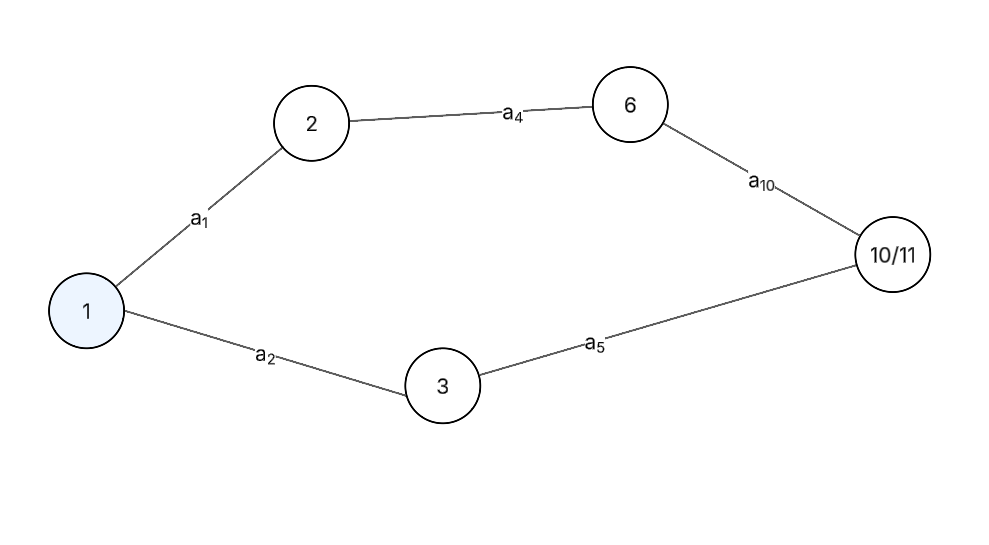
\includegraphics[width=0.425\textwidth]{figuras/contracao_novo_novo.png}
	\caption{Contração de vértice e vértice.}
	\label{fig:fusao}
\end{figure}

% Contração de dois vértices
% Contração de uma aresta


\chapter{Buscas}\label{cap:buscas}

A busca é umas das técnicas mais aplicadas na solução de problemas algorítmicos em grafos considerados eficientes. As duas técnicas de busca em grafos, a {dfs} e a {bfs}, são apresentadas, respectivamente, nas Seções \ref{sec:buscaLarg} e \ref{sec:buscaProf}.

A Seção \ref{sec:compFC} apresenta uma aplicação das duas buscas para obter os componentes fortemente conexos de um grafo. As considerações acerca da eficiência computacional, tanto em relação ao tempo de processamento quanto ao espaço usado de memória pelas buscas, são dadas na Seção \ref{sec:eficienciaRepresentacao}.

\section{Busca em Largura}\label{sec:buscaLarg}

\section{Busca em Profundidade}\label{sec:buscaProf}
A busca em profundidade serve para auxiliar algoritmos de verificação de grafos acíclicos, ordenação topológica e componentes fortemente conexos.
Como exemplo, foi feita uma busca em profundidade do grafo da Figura~\ref{fig:BusProf}, iniciando do vértice $V_1$ até o $V_2$.

Para realizar a busca, foi escolhida uma raiz ($V_1$) e, a cada vértice, um vértice filho para se seguir. 
O caminho utilizado foi:
\[
V_1 \rightarrow V_4 \rightarrow V_8 \rightarrow V_{12} \rightarrow V_{11} \rightarrow V_{15} \rightarrow V_{14} \rightarrow V_{13} \rightarrow V_9 \rightarrow V_6 \rightarrow V_2
\]

Após seguir para o $V_2$, é feito o retorno e verificado se todos os filhos estão na busca. Assim, surgem os vértices $V_{10}$, filho de $V_6$; $V_{16}$, filho de $V_{15}$; $V_3$ e $V_7$, filhos de $V_{11}$; e $V_5$, filho de $V_8$.

Também são analisadas as arestas de retorno (simbolizadas pelas linhas tracejadas na figura), que são arestas que ligam um vértice de tempo menor a um de tempo maior, sendo identificadas quatro:
\[
(V_2 \rightarrow V_1),\ (V_{10} \rightarrow V_{13}),\ (V_3 \rightarrow V_1),\ (V_7 \rightarrow V_{12})
\]

\begin{figure}[H]
	\centering
	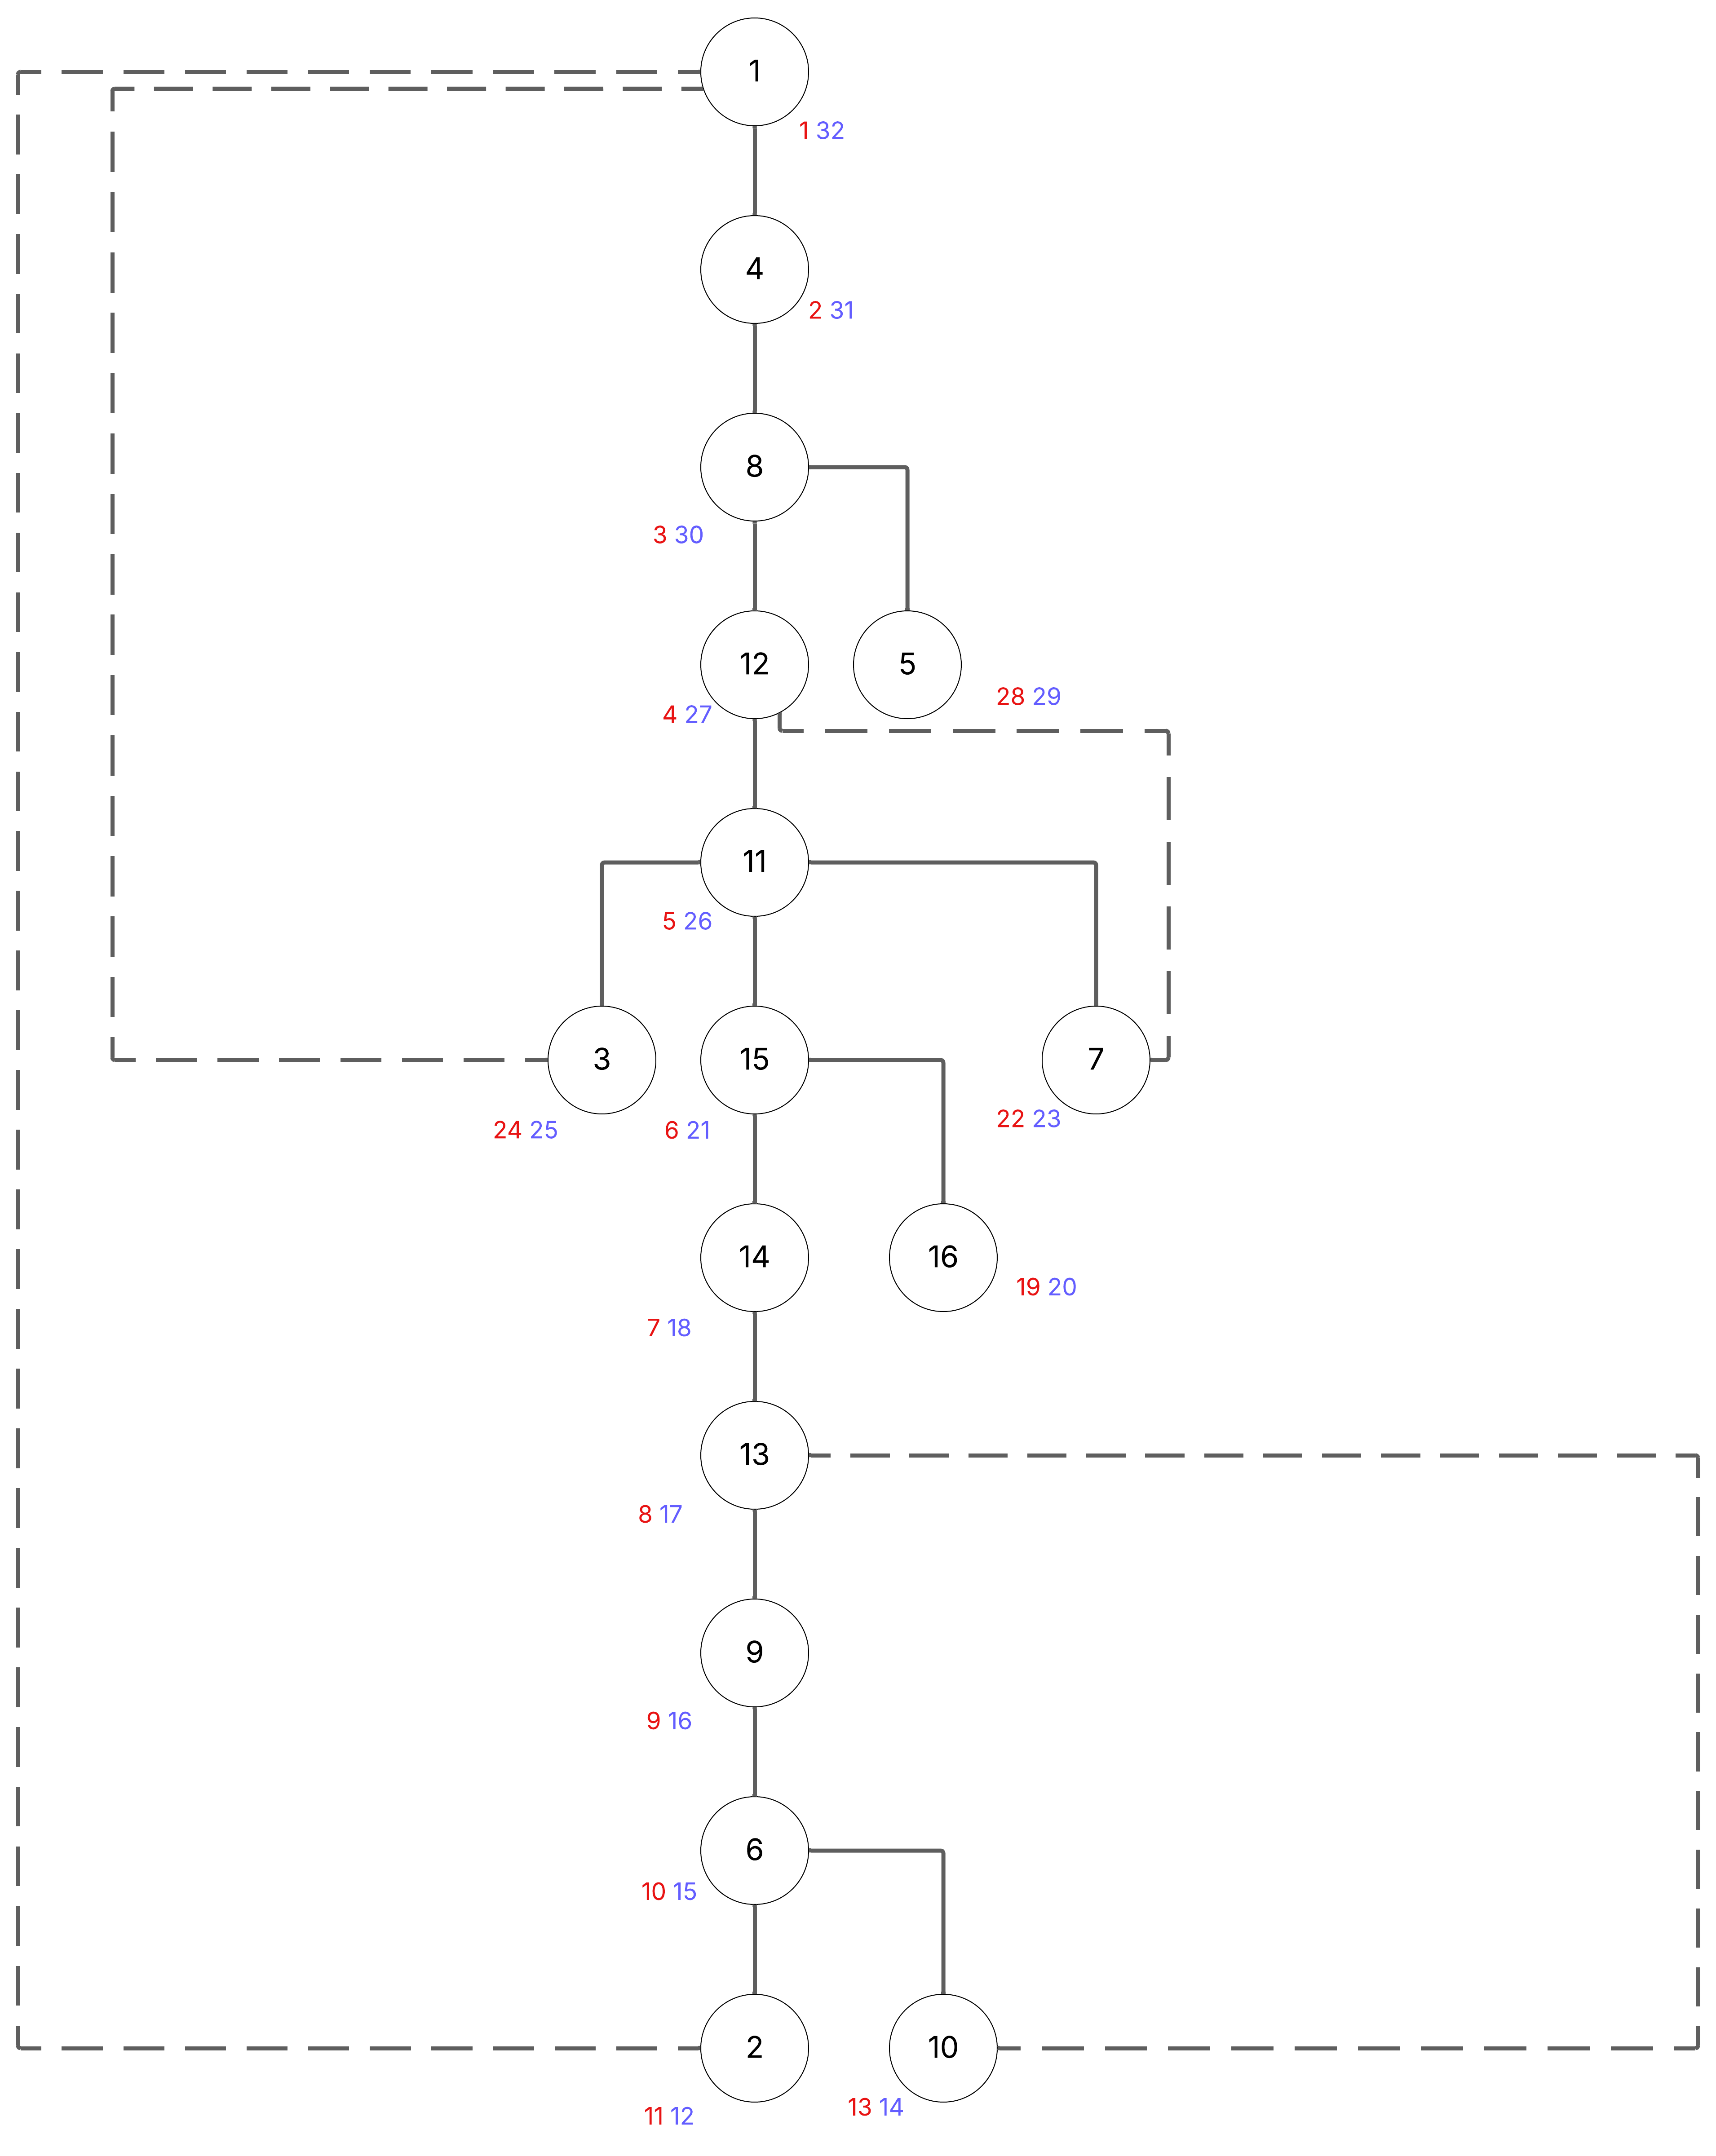
\includegraphics[width=0.425\textwidth]{figuras/BuscaProfundidade.png}
	\caption{Busca em profundidade}
	\label{fig:BusProf}
\end{figure}

\section{Componentes Fortemente Conexos}\label{sec:compFC}

% Considerações de Eficiência
\section{Considerações de Eficiência}\label{sec:eficienciaBusca}

\chapter{CAMINHO MÍNIMO}\label{cap:caminhoMinimo}


\chapter{ARVORE DE COBERTURA MÍNIMA}\label{cap:arvCobMinima}


\chapter{GRAFOS EULERIANOS}\label{cap:grafosEulerianos}


\chapter{GRAFOS HAMILTONIANOS}\label{cap:grafosHamiltonianos}


\chapter{EMPARELHAMENTO}\label{cap:emparelhamento}


\chapter{PLANARIDADE}\label{cap:planaridade}


\chapter{COLORAÇÃO DE VÉRTICES}\label{cap:coloracaoVertices}


% --- Referências (livre; substitua por biblatex se quiser)
\clearpage
\chapter*{REFERÊNCIAS}
\addcontentsline{toc}{chapter}{REFERÊNCIAS}
% Insira suas referências manualmente ou troque para biblatex.
\vspace{-0.5em}
\nocite{*}
\printbibliography[heading=none]

\end{document}